%% Document %%
\documentclass[12pt]{book}


%% Packages %%
\usepackage{breakcites}
\usepackage{ucs}
\usepackage{placeins} % donne \FloatBarrier pour forcer l'affichage de toutes les figures
\usepackage[utf8x]{inputenc}
\usepackage[francais]{babel}
%\usepackage{fullpage}
%\usepackage{mathpple}  % Pour la police
\usepackage{graphicx}
\usepackage{mathpazo}  % Pour la police

\usepackage{multirow} % lignes soudées

%\usepackage{multirow} % lignes soudées

\usepackage{hyperref}
\usepackage{amsmath}   % Pour numberwithin
%\usepackage{tocloft}   % pour cftsecaftersnumb ***
%\usepackage{spacing} \begin{spacing}{0.8} toto \end{spacing}
%\makeatletter \renewcommand{\numwidth}{9.55em plus1fil} \makeatother
\usepackage{fullpage}

%\usepackage{textcomp}
\usepackage[font={it}]{caption}

%\setcounter{tocdepth}{2}

%%%%%%%%%%%%%%% Modification de la taille des captions
% \newcommand{\captionfonts}{\small\itshape}
% 
% \makeatletter  % Allow the use of @ in command names
% \long\def\@makecaption#1#2{%
%   \vskip\abovecaptionskip
%   \sbox\@tempboxa{{\captionfonts #1: #2}}%
%   \ifdim \wd\@tempboxa >\hsize
%     {\captionfonts #1: #2\par}
%   \else
%     \hbox to\hsize{\hfil\box\@tempboxa\hfil}%
%   \fi
%   \vskip\belowcaptionskip}
% \makeatother   % Cancel the effect of \makeatletter
%%%%%%%%%%%%%%% Find de la modification


%% Metadata %%
\title{\Huge{Manuscrit de Thèse}\\\Large{Correction du mouvement respiratoire en TEP}}
\author{
        %\vspace{1cm}
        Simon Marache-Francisco \\
        Laboratoire CREATIS/LRMN - Philips Medisys
        %\vspace{1cm}
}
\date{\today}


%% Data %%
\begin{document}
\sloppy

% espace interr-paragraphe un peu plus grand
\addtolength{\parskip}{0.5em}


%\numberwithin{section}{part} 
%%%%%%% pour éloigner le texte de la tables des matières des nombres
%\renewcommand{\cftsecaftersnumb}{\hspace{1em}}
%\renewcommand{\cftsubsecaftersnumb}{\hspace{1em}}
%\renewcommand{\cftsubsubsecaftersnumb}{\hspace{1em}}

% ############################# Paramètres PERSO

\newcommand{\todo}[1]{
\addcontentsline{toc}{subsection}{\textbf{Todo:} #1}
$\|$\textbf{A Faire : }#1$\|$
}



\maketitle

\thispagestyle{empty}

%\begin{center}ù
%	\begin{tabular}{c c}
%		
\includegraphics[width=5cm]{images/logoPhilips} & 
\includegraphics[width=5cm]{images/logoCREATIS}
%	\end{tabular}
%\end{center}

%\vfill

\newpage

\tableofcontents


%\part{Introduction}
\newpage
\addcontentsline{toc}{part}{Introduction}
%\resizebox{4cm}{!}{\Huge Introduction}

{\fontsize{30}{100}\selectfont Introduction}

\rule{15cm}{0.1em}

\vspace{1cm}
\pagestyle{plain}

La tomographie par émission de positons (TEP) couplée à un tomodensitomètre (TDM) est une méthode d’imagerie clinique en forte expansion dans le domaine de l’oncologie. De nombreuses études cliniques montrent que la TEP permet, d’une part de diagnostiquer et caractériser les lésions cancéreuses à des stades plus précoces que l’imagerie anatomique conventionnelle, et d’autre part d’évaluer plus rapidement la réponse au traitement. Le raccourcissement du cycle comprenant le diagnostic, la thérapie, le suivi et la réorientation thérapeutiques contribue à augmenter le pronostic vital du patient et maîtriser les coûts de santé.

L’examen TEP/TDM au FDG apparaît désormais indispensable pour évaluer la réponse thérapeutique des patients atteints de lymphome. Les résultats préliminaires sont également très encourageants dans les tumeurs solides, en particulier les cancers pulmonaires, digestifs et de la sphère ORL~\cite{cachin2006evaluation}. La TEP pourrait prédire très précocement la réponse et ainsi permettre une réadaptation du schéma thérapeutique. Enfin de nouveaux traceurs TEP ouvrent la voie de l’imagerie moléculaire qui semble extrêmement prometteuse en thérapie génique et dans le suivi du traitement ciblé du cancer.

La durée d’un examen TEP, de l’ordre de 5 à 10 minutes pour un champ de vue axial de l’ordre de 15 cm, ne permet pas de réaliser une acquisition sous apnée. La qualité des images TEP est par conséquent affectée par les mouvements respiratoires du patient qui induisent un flou dans les images. Les effets du mouvement respiratoire sont particulièrement marqués au niveau du thorax et de l’abdomen. Deux types de méthodes ont été proposés pour corriger les données de ce phénomène. Le premier type est basé sur l’utilisation d’acquisitions synchronisées sur la respiration produisant plusieurs images non affectées par la respiration et correspondant à différents instants du cycle respiratoire~\cite{nehmeh2002effect}\cite{boucher2004respiratory}. Cette méthodologie se base sur l’hypothèse  d’une grande régularité du signal respiratoire de synchronisation~\cite{boucher2004respiratory}, et conduit à des images d’une qualité statistique limitée car chacune ne contient qu'une fraction réduite du nombre de photons détectés pendant toute l’acquisition~\cite{visvikis2004evaluation}. Le deuxième type de méthode se base sur l’utilisation d’un scanner 4D TEP/TDM du patient permettant de modéliser les mouvements respiratoires. Ce modèle est alors intégré lors du processus de reconstruction tomographique~\cite{lamare2007list}. Ce type de méthode permet de pouvoir conserver la statistique de l’image mais nécessite une information anatomique dynamique assez lourde à acquérir en routine clinique.

La problématique de la correction du mouvement respiratoire et le choix de la méthode appropriée sont des sujets d’actualité au sein de la communauté de médecine nucléaire. Des travaux récemment publiés proposent une évaluation de ces méthodes basée sur des critères de qualité tels que le rapport signal sur bruit ou le biais~\cite{visvikis2004evaluation}. Aucune étude à ce jour n’a évalué l’impact de ces corrections sur la qualité du diagnostic clinique. Ce problème pose des questions d’orientation stratégique et financière importantes, puisque le second type de méthode requiert l’acquisition de données TEP/TDM dynamiques, très peu accessibles à l’heure actuelle.

C'est dans l'optique de résoudre ce problème que j'ai commencé cette thèse sur l'\textbf{Estimation des apports de la correction du mouvement respiratoire en oncologie TEP}.


La première partie de ce manuscrit présente l'imagerie TEP. Nous détaillons les principes physiques de la TEP, le déroulement des acquisitions en nous focalisant sur l'imagerie TEP au $^18$FDG pour l'oncologie, et enfin les algorithmes de reconstruction utilisés pour former les images.

Ensuite, nous présentons un état de l'art sur le mouvement respiratoire, ainsi que son influence sur les lésions présentes dans les images TEP. Nous parlons ensuite des techniques permettant de l'estimer, puis de le corriger dans les images reconstruites.

La troisième partie porte sur les systèmes de détection automatisés, et dresse un état de l'art des méthodes d'évaluation des performances de détection. Nous présentons tout d'abord les bases de l'analyse psychophysique basée sur les courbes ROC (Receiver-Operating Characteristics), puis nous présentons les principe des sytèmes de détection automatique (CAD en anglais pour Computer-Aided Detection) que nous avons choisi d'utiliser dans cette étude, comme observateurs numériques en remplacement de l'observateur humain. Le dernier chapitre de cette partie présente et justifie les choix méthodologiques que nous avons faits pour répondre à la problématique clinique.

Enfin, nous présentons nos contributions : en premier lieu, la base de données, que nous avons créée pour réaliser les mesures de performances, puis nous décrirons la méthode utilisée pour répondre à la problématique, et enfin les résultats que nous avons obtenus.

La dernière partie correspond aux discussions et perspectives sur notre travail.	

\part{Imagerie TEP}
	La Tomographie par \'Emission de Positons (TEP) est une modalité d'imagerie fonctionnelle utilisant la désintégration d'un traceur radioactif pour mettre en valeur les zones de forte activité métaboliques. Elle est principalement utilisée en imagerie cérébrale, oncologie et cardiologie.

\chapter{Principe Physique}


	\section{Généralités}
L'imagerie TEP permet de visualiser de manière indirecte les désintégrations de particules survenant dans le corps du patient. Pour cela, on inject un ``traceur'' contenant une particule radioactive dans le corps du patient. Ce traceur est conçu de manière à se fixer sur les zones du corps que l'on souhaite imager. Pendant toute la durée de l'examen, les particules radioactives vont se désintégrer selon la loi de décroissance radioactive de la formule \ref{eq:loidecradioact}.

\begin{equation}
	dN = - \lambda N dt
	\label{eq:loidecradioact}
\end{equation}

$N$ représente le nombre le particules radioactives présentes dans le corps du patient. $dN$ représente la variation de ce nombre de particules (le nombre de désintégrations par $dt$) et $\lambda$ est une constante dépendant de l'élément radioactif.

Chaque désintégration d'un élément radioactif va déclencher l'émission d'une particule $\beta$, aussi appellée positon. En oncologie, on utilise le Fluor $^{18}F$ qui se désintégre en Oxygène $^{18}O$ en émettant le positon. Cette particule va parcourir quelques mm avant de s'annihiler avec un élection en émettant 2 photons dans deux directions opposées avec une énergie de 511 KeV.

Ce seront ces photons qui vont être détectés par l'imageur TEP pour reconstituer la position de la désintégration initiale. 
	\subsection{Détecteur}

Les détecteurs utilisés en TEP sont constitués d'un matériau photomultiplicateur placé devant un capteur. Chaque photon va entraîner un qui va déclencher une émission lumineuse à cahque photon détecté, placé à cotésuivi par un détecteur qui va convertir cette émission lumineuse en impulsion électrique. 

	\section{perturbation trajet du photon}

		\subsection{Diffusion}
		
		\subsection{Déviation}
		
		\subsection{Absorbtion}

\chapter{Déroulement d'une acquisition}
	\section{2D / 3D}
	\section{Format des données}
Les données acquises par une caméra TEP peuvent être stockées sous deux formes principales : Sinogramme et list-mode.
		\subsection{List-mode}

Ce format correspond à un enregistrement ``brut'' des données issues de l'électronique de la caméra.

Ce format de fichier est en fait un enregistrement séquentiel des évènements, dans leur ordre de détection. On peut enregistrer chaque détection indépendamment, ou encore uniquement les coïncidences. Les évènements sont datés, ce qui permet de conserver l'informations temporelles. 

Il existe plusieurs formats de fichiers pour le stockage de ces données, notamment le format LMF (List-Mode Format) développé pour le projet ClearPET et le format ROOT développé par le CERN. 

L'avantage de ces formats est qu'ils permettent de conserver les informations sur la dynamique de l'acquisition, mais aussi qu'ils permettent le stockage de métadonnées utiles en simulations, notamment le nombre de diffusions, ou de marquer les coincidences fortuites.

		\subsection{Sinogramme}

Le sinogramme est une image 
\chapter{Algorithmes de reconstruction}
	\section{Itératifs}
		\subsection{EM}
		\subsection{OSEM}
	\section{Analytiques}
	
			
%	\chapter{Imagerie TDM}

\part{Mouvement respiratoire}
%	\chapter{Modalités d'imageries}
%	
\section{Tomographie par émission de positons (PET)}

\subsection{Historique}

\subsection{Principe physique}

\subsection{Reconstruction des images}

\section{Tomodensitométrie}

La tomodensitométrie (TDM) est une technique d'imagerie utilisant les rayons X pour imager l'atténuation des tissus. Ils sont transmis d'une source sur un détecteur à travers le corps humain et renseignent sur les différentes atténuation des tissus présents. Des algorithmes de reconstruction analytiques ou itératifs (fedkampf)


\subsection{Historique}

\subsection{Principe physique}



\subsubsection{Physique}

\subsection{Reconstruction des images}




	\chapter{Respiration et influence sur les acquisitions TEP/TDM}
	Le mouvement respiratoire en imagerie TEP engendre plusieurs effets sur les images reconstruites, qui seront détaillés ci-après. Ils occasionnent notamment une diminution de la qualité des images, ce qui peut perturber le travail des praticiens.

\section{Mouvement respiratoire}

Ce mouvement est la succession d'une phase inspiratoire, suivi d'une phase expiratoire. Chacune de ces phases combine plusieurs mouvements élémentaires~\cite{servant2007cours} :
 
\begin{enumerate}
 \item thoracique, avec un déplacement des côtes
 \item abdominal, avec un déplacement du diaphragme
 \item en cas d'inspiration forcée, action des pectoraux
\end{enumerate}

La figure~\ref{fig:respiXCAT} représente 3 instants du cycle respiratoire utilisé dans le NCAT, un modèle de corps humain respirant. On voit clairement tous les effets présentés précédemment, notamment le relèvement des côtes et du sternum à l’aide des guides présents sur les images.

\begin{figure}[h!]
    \begin{center}
            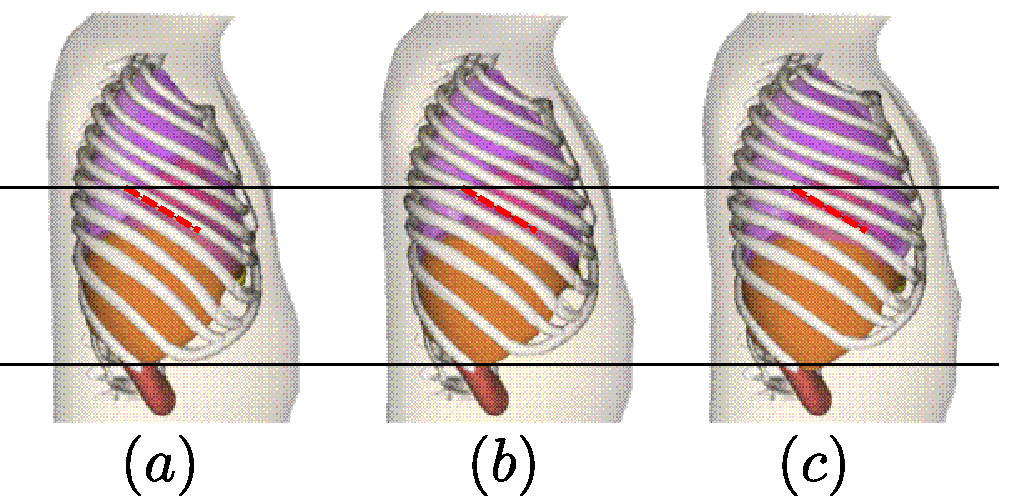
\includegraphics[width=10cm]{images/mvtRespi} \\
    \end{center}
    \caption[Modèle de mouvement intégré dans le fantôme NCAT]{Modèle de mouvement intégré dans le fantôme NCAT. La ligne pointillée rouge sert de référence pour la position d'une des côtes du modèle en expiration. L'image (a) correspond à l'expiration complète, et la (c) à la fin de l'inspiration. (b) correspond à un instant intermédiaire du cycle. }
    \label{fig:respiXCAT}
\end{figure}


La variabilité inter et intra-patient de ce mouvement est très importante : le volume d'air inspiré peut varier de 500 mL à 1200 mL selon que la personne a une respiration normale ou profonde. Pour ces deux extrêmes, la fréquence respiratoire varie de 5 cycles/min. à 20 cycles/min.~\cite{sherwood2006fundamentals}.

Or une acquisition TEP a une durée de plusieurs minutes par lit, ce qui amène à la reconstruction d'une image dégradée, notamment au niveau de la localisation de la tumeur, de son activité mesurée et, par extension, de sa détection. De la même manière, des artefacts apparaissent au niveau des zones de fort mouvements dans les images TDM, lorsque les organes bougent pendant une rotation du détecteur.

Je vais tout d'abord introduire les effets visibles sur les images, puis je m'attarderai sur les mesures quantitatives utilisées pour mesurer l'apport de la correction du mouvement sur les tumeurs. Ensuite, dresserai un état de l'art plus précis des publications s'intéressant à l'impact du mouvement respiratoire sur la détection.

\section{Localisation et Volume}


La localisation et le volume des tumeurs peuvent être modifiés par le mouvement engendré par la respiration (voir figure~\ref{fig:effetMvt}). D'après l'étude de~\cite{lamare2007respiratory}, réalisé sur des simulations Monte-Carlo à l'aide du logiciel de simulation GATE~\cite{jan2004gate} en utilisant le modèle NCAT~\cite{segars2001These}, la largeur à mi-hauteur des lésions peut être modifiée de 48\% (équation~\ref{eq:PRD} : Différence relative) dans le cas d'une lésion de 7mm de diamètre dans la partie basse du poumon. L'imprécision axiale sur le positionnement de la tumeur peut atteindre 9\% dans les mêmes conditions.

\begin{equation}
\%DR= \left| \frac{Crit\grave{e}re~sur~image~non~corrig\acute{e}e - Crit\grave{e}re~sur~image~de~r\acute{e}f\acute{e}rence}{Crit\grave{e}re sur image~de~r\acute{e}f\acute{e}rence} \right|
\label{eq:PRD}
\end{equation}


\begin{figure}[h!]
    \begin{center}
            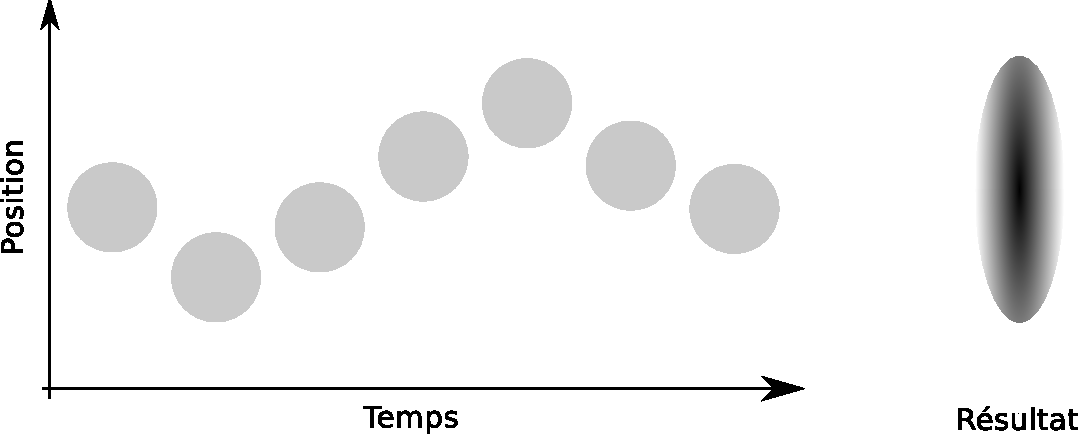
\includegraphics[width=10cm]{images/moyennageImage} \\
    \end{center}
    \caption[Effet du déplacement d'une tumeur sur les données acquises]{Effet du déplacement d'une tumeur sur les données acquises. La position de la tumeur change en fonction du temps, ce qui provoque l'acquisition d'une tumeur équivalente présentée à droite.}
    \label{fig:effetMvt}
\end{figure}


\section{Mesure de l'activité des tumeurs}

Le contraste des tumeurs par rapport au fond est un critère important pour déterminer la malignité des tumeurs~\cite{dimitrakopoulou2002role, krak2005effects}. Ce contraste joue ausi un rôle important sur la détectabilité de la tumeur en facilitant sa détection, comme nous allons le voir ci-après.

L'activité peut être influencée par la respiration de deux manières : par un mauvais ajustement de la carte d'atténuation, et par le moyennage de la position de la tumeur.

\subsection{Décalage de la carte d'atténuation}

\todo{définir le SUV quelquepart}

La carte d'atténuation utilisée pour corriger les images d'émission est basée sur une image TDM prise à un instant donné du cycle. Or l'atténuation de la zone correspondant à une tumeur peut être différente de celle des tissus environnants, ce qui peut occasionner des sous-estimations ou de sur-estimation de l'activité de la tumeur si la carte d'atténuation est mal positionnée.

D'après l'étude~\cite{erdi2004ct} réalisée sur cinq patients, on peut observer des variations très importante de $SUV_{max}$ (voir équation~\ref{eq:varSUV}) sur les images TEP reconstruites. L'étude a été réalisée sur 5 patients totalisant 8 lésions. L'acquisition TDM 4D a été synchronisée sur le mouvement à l'aide d'un dispositif placé sur l'abdomen du patient. Ce dispositif était constitué de 2 marqueurs réfléchissant les ondes infrarouges, placés dans le champ de vue d'une caméra. Les données synchronisées acquises en TDM 4D ont été utilisées pour générer un cycle de 10 images TDM. Chacune de ces 10 images a ensuite servi de carte d'atténuation lors de la reconstruction des images d'émission, générant ainsi 10 images TEP .

Les données TEP reconstruites à partir des 10 images ont montrés de grandes différences en termes de SUV selon l'instant du cycle à partir duquel les lésions ont été extraites.
Ces variations allant jusqu'à 24\% pour une lésion de $19.8~mm^3$ placée dans l'espace médiastinal, entre une reconstruction TEP réalisée à partir d'une image TDM de fin d'expiration et une image TDM de fin d'expiration. En recherchant la variation la plus grande sur l'ensemble du cycle (en non pas en se limitant aux extrêmes), la variation peut atteindre 30\%.

La figure~\ref{fig:lesionEnFctPhaseTDM} présente la variation de $SUV_{max}$ en fonction de la phase utilisée pour la reconstruction.

\begin{equation}
\label{eq:varSUV}
 \%~variation~SUV_{max} = 100 \times \frac{ | SUV_1 - SUV_2 | }{ (SUV_1 + SUV_2) / 2 }
\end{equation}

\begin{figure}[h!]
	\vspace{0.5cm}
	\centering
			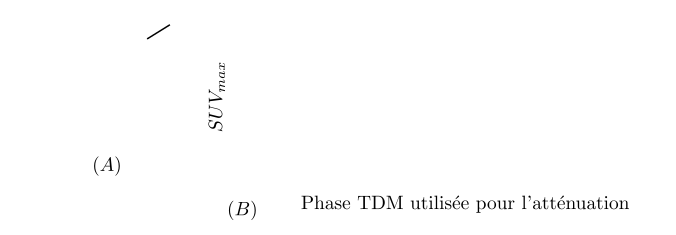
\includegraphics[width=10cm]{images/lesionEnFctPhaseTDM}
	\vspace{-0.5cm}
	\caption[Influence de l'influence de la carte d'atténuation sur l'activité des lésions] {A) Vue coronale d'un patient avec une lésion clairement visible en haut à droite (flèche noire).  B) $SUV_{max}$ observé sur les images reconstruites en fonction de l'image TDM utilisée pour la reconstruction. Le nombre en abscisse représente la position dans le cycle respiratoire en pourcentage.} 
	\label{fig:lesionEnFctPhaseTDM}
\end{figure}

\subsection{Artefacts TEP dus aux artefacts TDM}

On peut voir sur les images de la figure~\ref{fig:artefactsCT} des artefacts présents sur les images TDM utilisées pour la correction d'atténuation. Ces artefacts proviennent de la manière dont les images sont acquises : la caméra tourne autour du sujet dans un mouvement hélicoïdal, et l'algorithme de reconstruction va ensuite utiliser les acquisitions pour reconstruire une image complète. Or en cas de respiration rapide, des incohérences peuvent survenir quand le mouvement du diaphragme est plus important que celui de la caméra. Ce type d'artefacts peut créer des incohérences dans les images TEP reconstruites.

\begin{figure}[h!]
	\begin{center}
		\begin{tabular}{c c}
			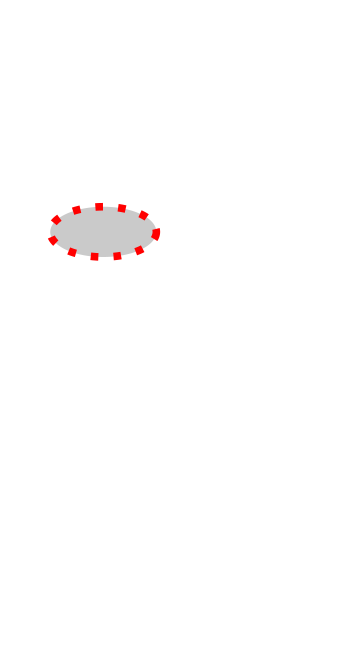
\includegraphics[width=5cm]{images/artefactCT1} & 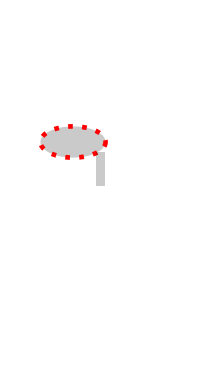
\includegraphics[width=5cm]{images/artefactCT2}
		\end{tabular}
	\end{center}
	\caption{Artefacts présents sur des images TDM utilisées pour la correction d'atténuation} 
	\label{fig:artefactsCT}
\end{figure}


\subsection{Déplacement de la tumeur au cours du cycle}

Le mouvement respiratoire va avoir pour effet de déplacer la tumeur pendant l'acquisition, ce qui va moyenner la quantité de radioactivité sur l'ensemble du cycle, comme indiqué sur la figure~\ref{fig:effetMvt}. Si le déplacement de la tumeur est suffisamment grand par rapport à son diamètre, la réduction de radioactivité va être importante.

L'étude~\cite{boucher2004respiratory} réalisée sur un fantôme elliptique (modèle ``Elliptical Jaszczak Phantom'') montre qu'un déplacement d'une source radioactive de 6 mm sur un cycle respiratoire moyen entraîne une sous-estimation de l'activité maximale de la tumeur de 41\% pour une lésion de 1.2 ml et de 21\% pour une sphère de 19.4 ml.


\section{Impact du mouvement respiratoire sur la détection}

Peu de travaux ont été réalisés sur l'impact du mouvement respiratoire sur la détection des tumeurs. Globalement, les critères utilisés sont principalement des mesures orientées sur la quantification des lésions ($SUV_{max}$, profils de lésions, ...). Très peu d'articles utilisent des critères orientés sur les performance de détection.

Voici une liste des critères utilisés dans différentes publications pour évaluer les performances d'algorithmes de correction du mouvement respiratoire :

\begin{enumerate}
 \item  $SUV_{max}$, contraste :~\cite{GuopingChang2010Implementation,lamare2007list,nehmeh2002effect,detorie2008quantitative}
 \item Visualisation des Profils de lésion :~\cite{GuopingChang2010Implementation,Thielemans2006Lesion,lamare2007list}
 \item Volume et position de la lésion :~\cite{GuopingChang2010Implementation,lamare2007list,nehmeh2002effect}
 \item Rapport signal sur bruit (SNR) :~\cite{GuopingChang2010Implementation}
 \item Observateur de Hotelling (CHO) :~\cite{Thielemans2006Lesion}
\end{enumerate}

Comme on peut le voir, les deux seuls critères qui pourraient s'approcher d'une étude sur la détection sont le SNR et le CHO, mais ils sont largement sous-représentés. 

Je vais me concentrer sur les deux publications qui utilisent un observateur, et présenterai les résultats des autres publications dans la partie suivante.

Un autre document par Rahmim Arman~\cite{rahmim4d} propose d'utiliser le CHO pour évaluer l'amélioration de la détection des défauts dans de l'imagerie cardiaque corrigée du mouvement respiratoire. Ce document n'a pas encore donné lieu à publication.

\subsection{Synthèse de Thielemans,2006}

\todo{voir ce que c'est que cette histoire avec l'autre citer thielemans}

Dans sa publication, Thielemans~\cite{Thielemans2006Lesion} utilise le ``Channelized Hotelling Observer'' (CHO)~\cite{barrett1993model}, qui est un observateur dérivé du classifieur linéaire LDA présenté en \ref{lab:LDA}, utilisé en conjonction avec des informations fréquentielles. 

Cependant ils utilisent le CHO uniquement sur des lésions de fort diamètre et de fort contraste (13mm de diamètre et contraste de 4.25:1, sur des simulations analytiques). Les résultats présentés (figure~\ref{fig:apportCHO}) montrent une amélioration du score pour les méthodes de correction de l'ordre de 50\% dans certains cas. 

Mais il est difficile d'évaluer de manière précise l'apport des méthodes de détection à l'aide de ces seuls ``scores'' car ce sont des résultats qualitatifs. 

\begin{figure}[h!]
	\begin{center}
			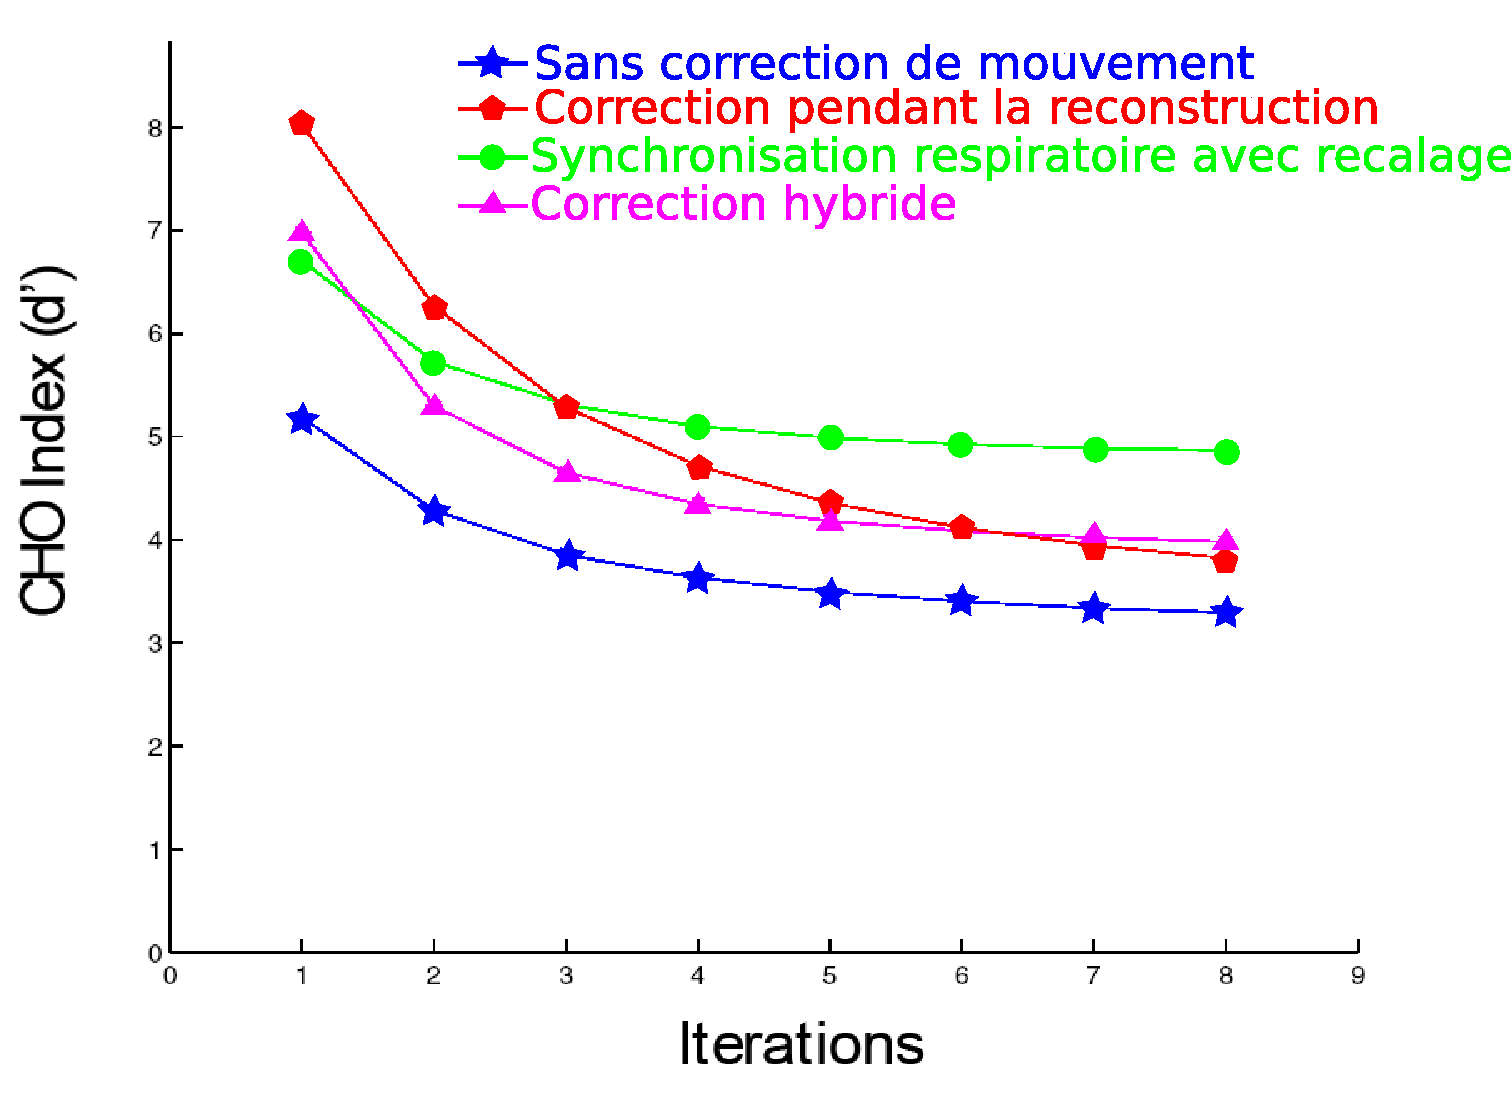
\includegraphics[width=10cm]{images/apportCHO}
	\end{center}
	\caption[Index de CHO pour différents techniques de correction du mouvement respiratoire en fonction du nombre d'itérations]{Index de CHO pour différents techniques de correction du mouvement respiratoire en fonction du nombre d'itérations. La méthode utilisant le gating est comparée avec une méthode évolution présentée dans le document.} 
	\label{fig:apportCHO}
\end{figure}


\subsection{Chang 2010}

Cette publication est une évaluation clinique d'un système de découpage automatique du signal respiratoire par amplitude. Elle est basée sur 13 patients totalisant 21 tumeurs du poumon de taille diverses (estimée de 1 à 27 $cm^3$. Le signal respiratoire est acquis à l'aide d'un dispositif propriétaire (Anzai AZ-733V) basé sur une ceinture abdominale avec capteur de pression. Seuls les données TEP acquises autour d'une amplitude présélectionnée (+/-10\% de l'amplitude correspondant à l'acquisition TDM) sont utilisées pour la reconstruction des images corrigées. 

Le jeu d'images ``témoin'', non corrigées, est réalisé en extrayant des données acquises le même nombre d'évènements N que le jeu d'images synchronisées en considérant les N premiers du fichier en mode séquentiel.

L'auteur compare le $SUV_{max}$, $SUV_{moyen}$, Rapport Signal/Bruit (SNR) et volume apparent de la lésion pour les deux jeux d'images. Le volume de la lésion et le $SUV _{moyen}$ sont calculés sur une région d'intérêt correspondant à 40\% du $SUV_{max}$ de la lésion. Le SNR est calculé en divisant le SUV moyen de la tumeur par l'écart-type d'une zone d'intérêt dans le poumon, dont ni la taille ni la localisation ne sont précisées. 

Les résultats présentés montrent une amélioration importante des valeurs du SNR pour les images corrigées du mouvement par rapport aux images témoin, comme présenté dans la figure~\ref{fig:guoping2010Exemple}. En moyenne, cette augmentation est de 26.3\%, mais deux tumeurs sur les 21 de l'étude voient leur SNR augmenter de plus de 66\%. 

\begin{figure}[h!]
	\begin{center}
			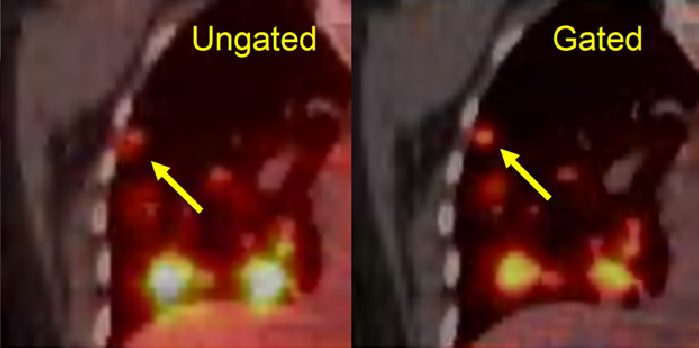
\includegraphics[width=10cm]{images/guoping2010Exemple}
	\end{center}
	\caption{Exemple d'image avec et sans correction de mouvement respiratoire.} 
	\label{fig:guoping2010Exemple}
\end{figure}




Il est étonnant de constater que les mesures moyennes sur les 21 tumeurs de $SUV_{max}$ et $SUV_{moyen}$ voient leurs valeurs augmenter respectivement de 26.8\% et 26\%, ce qui est tout à fait semblable avec l'augmentation de SNR. Cependant, les valeurs individuelles d'amélioration  pour chaque tumeur ne montrent pas de corrélation avec le SNR. Par exemple, une lésion va montrer une augmentation de 24\% de son $SUV_{max}$, de 20\% de son $SUV_{moyen}$ et de 37\% de son SNR.

Il est intéressant de constater qu'il y a un point où le SNR diminue de 3.4\%, mais que le $SUV_{max}$ et le $SUV_{moyen}$ augmentent tout de même de presque 18\%. Cela semble indiquer une erreur car le SUV de la zone d'intérêt n'est pas censé changer de manière importante.

	
	\chapter{Processus d'estimation du mouvement}
	\section{Estimation du signal respiratoire}

Le signal respiratoire est une grandeur qui permet de positionner le cycle entre la fin d'inspiration et la fin d'expiration. Il est habituellement fourni par des capteurs externes qui génèrent un signal qui sera corrélé avec la respiration. Cela permet de faire correspondre les données acquises par un imageur avec une phase particulière du mouvement respiratoire.

\subsection{Spiromètre}
\label{lab:spirometre}
Le spiromètre est un capteur externe placé sur la bouche du patient et qui permet de mesurer les déplacements d'air dans le système respiratoire~\cite{guivarc2004synchronization}. Les spiromètres mesurent un débit ou un volume d'air inspiré/expiré (voir illustration figure~\ref{fig:spirometre}). A partir de l'une des grandeurs, il est possible d'estimer l'autre facilement. L'avantage du spiromètre est qu'il permet d'accéder à une mesure caractérisant directement la respiration du patient, et n'est pas sujet à des perturbations externes (mouvements involontaires par exemple). Par contre cela demande un appareillage qui peut être assez invasif pour le patient.

\begin{figure}[h!]
	\begin{center}
		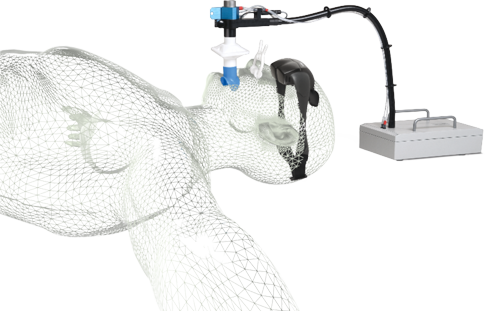
\includegraphics[width=12cm]{images/spiro}
	\end{center}
	\caption{spiromètre Syn'r : on peut voir le système de mesure de la respiration ainsi qu'un système de moniteurs implantés dans les lunettes pour aider le patient à contrôler sa respiration} 
	\label{fig:spirometre}
\end{figure}

\subsection{Ceinture}

Pour mesurer le signal respiratoire, il est possible d'utiliser un capteur qui va mesurer le périmètre du thorax. L'extension de cette ceinture va correspondre aux mouvements de la cage thoracique et de l'abdomen pendant la respiration du patient. C'est une mesure indirecte de l'amplitude du mouvement respiratoire utilisée couramment en routine clinique. 

Différentes technologies existent pour mesurer cette information (RespiTrace R250 de Studley. Data Systems, Respiratory Belt Transducer de ADInstruments, ...). Elles sont basées sur plusieurs effets (résisitif, inductif...) et ont l'avantage d'avoir un faible coût et de ne pas perturber le patient.

Bien qu'elles puissent être influencées par les mouvements involontaires du patient, il a été montré dans~\cite{Guivarch2004Sync} que les données acquises selon les méthodes par respiromètre et par ceinture sont équivalentes.

\subsection{Basés caméras}

Des caméras peuvent être utilisées pour estimer le mouvement respiratoire. Une des techniques consiste à utiliser des informations surfaciques en reconstruisant en 3D certaines parties du corps à l'aide de plusieurs caméras (avec ou sans marqueurs) ou de caméra temps de vol. Cela permet d'avoir plus d'informations sur la respiration.

Une autre technique consiste à installer un marqueur sur le corps du patient et de relever les déplacements de ce marqueur sur plusieurs axes à l'aide d'une caméra. Un tel système est décris dans~\cite{nehmeh2002effect} : Respiratory Gating System de Varian Medical Systems (voir figure~\ref{fig:RGSdeVarian}).

\begin{figure}[h!]
	\begin{center}
		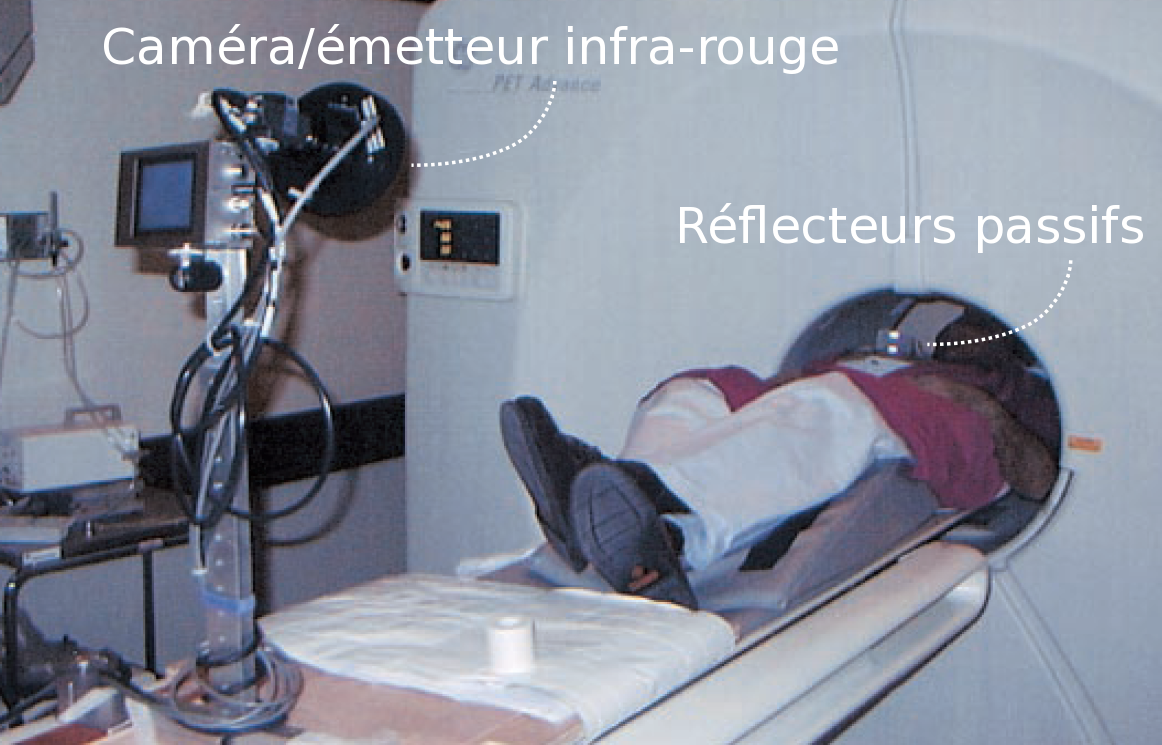
\includegraphics[width=12cm]{images/varian}
	\end{center}
	\caption{Photographie du système RGS de Varian medical Systems en action : une caméra va détecter le déplacement d'une zone du thorax en mesurant le déplacement de marqueurs placés sur un bloc plastique.} 
	\label{fig:RGSdeVarian}
\end{figure}

Ces techniques ont l'avantage d'être moins invasives et plus facilement acceptées par le patient. Cependant, elles sont beaucoup plus sensibles aux mouvements involontaires du patient. Pour l'acquisition d'image TDM ce risque est faible car elles sont de faible durée (inférieures à la minute), mais il devient important pour les acquisitions TEP qui peuvent durer en tout plusieurs dizaine de minutes. Ces mouvements n'étant probablement pas corrélés avec le mouvement respiratoire, ils vont perturber le signal obtenu. 

\subsection{Techniques basées sur les images TEP}
\label{lab:estimMvtTEP}
En TEP, la publication de Bundschuh et al.~\cite{bundschuh2007postacquisition} utilise les données dynamiques pour estimer le signal respiratoire sans avoir besoin de capteur externes . Ce processus est réalisé en 5 étapes : 

\begin{enumerate}
 \item Les données TEP sont acquises en mode séquentiel : toutes les désintégrations détectées sont enregistrées dans un fichier de manière séquentielle  
 \item L'image TEP statique est reconstruite. Elle permet de localiser une lésion dans l'image qui servira d'amer pour l'estimation du mouvement respiratoire.
 \item Une image TEP est reconstruite pour chaque intervalle temporel de 0.5 secondes.
 \item La zone d'intérêt sélectionnée précédemment est sélectionnée dans chaque image reconstruite. La position axiale du barycentre à chaque instant temporel va donner une estimation du mouvement respiratoire pour le volume donné.
\end{enumerate}

Cette technique a été évaluée sur 10 patients et les signaux ont été comparés avec ceux obtenus avec des ceintures abdominales. Pour 3 patients, les courbes respiratoires obtenues par les deux techniques étaient très fortement corrélées. Pour deux autres patients, l'estimation de mouvement obtenue par la TEP était trop bruitée, mais montrait une bonne corrélation avec le signal obtenu par les ceintures abdominales après filtrage. Pour 3 autres patients, il n'a pas été possible de trouver une corrélation entre les deux signaux. Les deux derniers patients ont bougés pendant l'acquisition TEP, ce qui a perturbé le signal.

Cette technique est intéressante mais contrainte par la qualité de l'image TEP. En pratique, la moitié des acquisitions de signaux n'ont pas permis d'obtenir un signal satisfaisant.


\section{Estimation du champ de mouvement}
\label{lab:estimChamp}
Le champ de mouvement est une information beaucoup plus riche que le signal respiratoire car il permet de suivre les déplacements des organes et des lésions à l'intérieur du corps du patient à l'intérieur d'un cycle respiratoire.

Le signal respiratoire acquis par les méthodes précédemment cités est utilisé pour décomposer les données acquises en TDM ou TEP en plusieurs phases, chacune correspondant à un instant du cycle. Ces informations sont utilisées pour assembler les données acquises pour chaque phase, reconstruites indépendamment. Ces reconstructions vont être utilisées pour estimer le champ de mouvements à l'aide de techniques de recalage.


\subsection{Image TEP 4D}
\label{lab:estimMvtTEP4D}
L'estimation du champ de mouvement respiratoire peut être fait à partir des données TEP, comme il a été montré par~\cite{dawood2008respiratory, dawood2006lung}. 

Les techniques utilisées sont analogues à celle présentée en~\ref{lab:estimMvtTEP}. Elles consistent à réaliser une acquisition list-mode des données en même temps qu'une acquisition du signal respiratoire, puis à réorganiser les données acquises pour reconstruire les différents instants du cycle indépendamment et sans correction d'atténuation. Le mouvement sera estimé à partir de ces images.

La publication de~\cite{dawood2008respiratory} cherche à corriger le mouvement respiratoire, et pour cela fait une estimation préliminaire de ce mouvement. 

Pour obtenir le signal respiratoire, dawood utilise une caméra qui enregistre le mouvement d'un marqueur placé sur l'abdomen du patient. Ce marqueur est un point blanc placé sur un disque noir, et sa position axiale est détectée par seuillage. 

La synchronisation avec l'acquisition PET est réalisée à l'aide d'une LED dans le champ de vue de la caméra qui s'allume lors du début de l'acquisition. Une fois l'acquisition réalisée, le signal respiratoire obtenu est utilisé pour répartir les évènements acquis par l'imageur sur un seul cycle respiratoire. Ce cycle est décomposé en 8 parties qui seront reconstruites séparément, sans correction d'atténuation. 

Les auteurs utilisent ensuite un algorithme de flux optique 3D présenté dans~\cite{dawood2006lung} et~\cite{horn1981determining} pour déterminer le champ de mouvement : Ils estiment un déplacement entre chaque image du cycle et l'image de référence (la 4è dans le cas de cet article). Le résultat de l'algorithme sera donc une séquence de champ de mouvement formant un champ de déformation 4D.

L'algorithme a été testé sur le fantôme XCAT ainsi que sur les données de 16 patients. La performance de l'estimation de mouvement a été évaluée selon trois critères, évalués sur les images corrigées : la correction du déplacement axial du coeur, le coefficient de corrélation des images corrigées du mouvement, ainsi que le bruit obtenu. Je présenterais ces résultats dans la présentation de cet article dans la partie~\ref{lab:correctionDawood2008}.

Bai a présenté une technique d'estimation semblable~\cite{bai2009regularized}. Le principe est le même que pour la publication précédente, mais en réalisant une estimation du mouvement à l'aide de B-splines~\cite{thevenaz2000optimization}.

Un exemple de champ de déformation obtenu est présenté en~\ref{fig:champMouvementBai}

\begin{figure}[h!]
	\begin{center}
		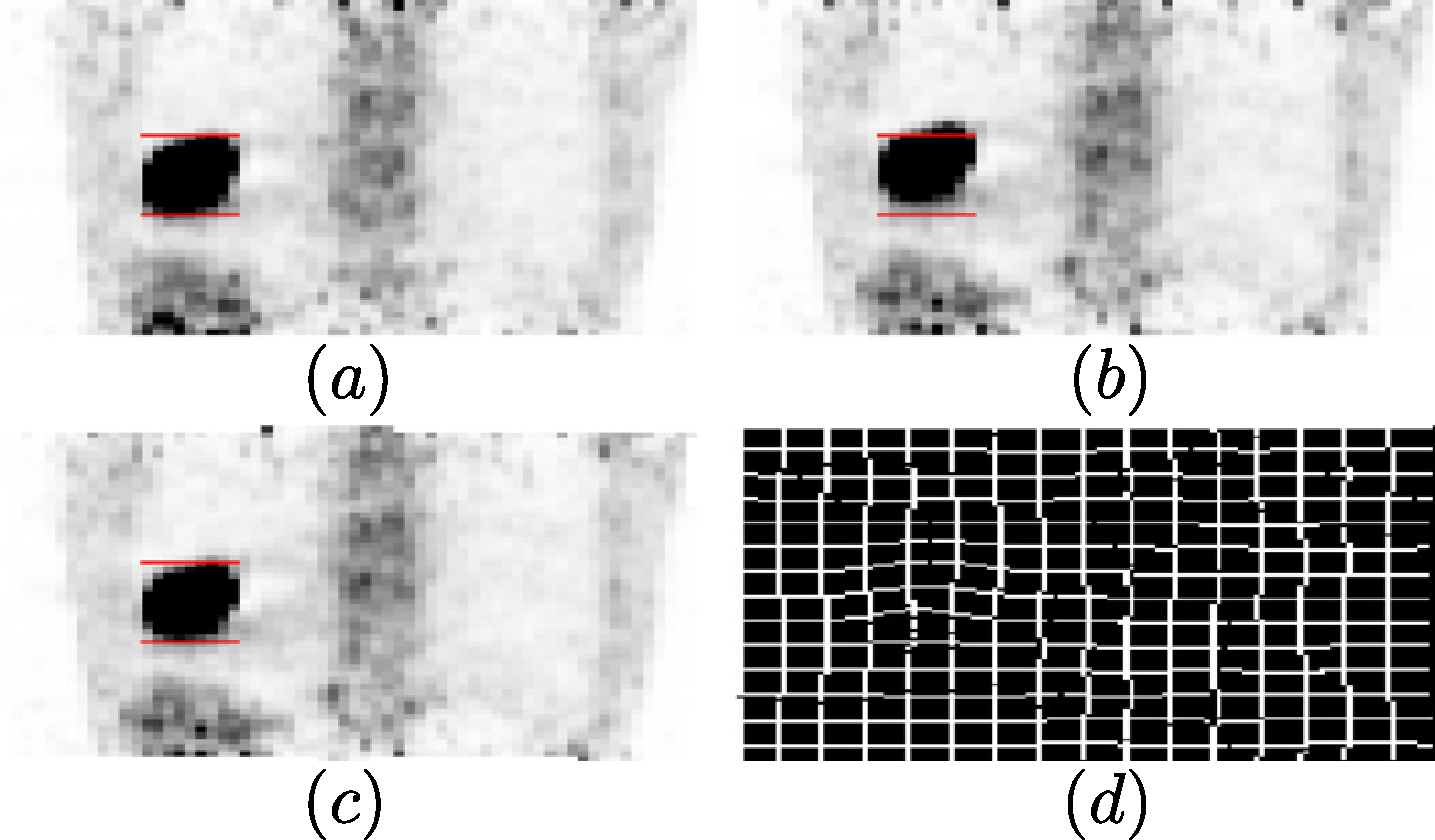
\includegraphics[width=12cm]{images/champDeformBai2}
	\end{center}
	\caption{Champ de déformation calculé à l'aide de la méthode présenté en~\cite{bai2009regularized}. a) représente l'image TEP obtenue à partir des données de la phase de référence  (mi-expiration), b) correspond à l'image reconstruite pour les donnée d'expiration complète, et c) le résultat du recalage de l'image de fin d'expiration sur l'image de référence. d) représente le champ de mouvement résultat. Les traits rouges représentent l'extension axiale de la tumeur dans l'image de référence.} 
	\label{fig:champMouvementBai}
\end{figure}

\subsection{Image TDM 4D}

Les images TDM peuvent être acquises en mode dynamique de manière à obtenir une suite d'images couvrant tout le cycle respiratoire~\cite{lamare2007list, qiao2006motion}. Les données sont reconstruites indépendamment, avec un rapport sur bruit plus faible que sur l'image originale. 

Des algorithmes de recalage sont utilisés de manière à déduire le champ de mouvement. Le principal avantage de l'utilisation des images TDM 4D est la précision des images. En effet, alors que les images TEP ont une résolution de l'ordre de 5mm, les images TDM atteignent des résolutions inférieures au mm, ce qui permet d'obtenir un champ de mouvement beaucoup plus précis. Cependant, utiliser des images TDM 4D a plusieurs inconvénients :

\begin{itemize}
 \item Une possible incohérence entre le cycle acquis en TDM 4D et la respiration du patient en TEP. Bien que les imageurs TEP/TDM couplent les deux imageurs sur la même machine, de manière à éviter les mouvements du patients entre les acquisitions, le cycle acquis en TDM ne représente qu'un cycle, tandis que l'acquisition TEP va donner un ``cycle moyen`` plus proche de la réalité.
 \item Une dose de radiation émise plus importante. Bien que les technologies récentes permettent de réduire les doses de manière importante pour l'acquisition dynamique, elles restent tout de même plus importantes que pour un CT 3D.
\end{itemize}

Il faut noter que plusieurs publications basées sur des simulations se servent des cartes de labels utilisées pour la simulation pour réaliser les estimation de mouvements~\cite{lamare2007list}. Cela donne une estimation dans le ``meilleur des cas'', où l'image TDM est parfaitement en phase avec les images TEP.

\section{Modèle}

Une autre voie est en cours de développement basée sur la création d'un modèle de respiration qui est adapté à chaque patient à partir d'une quantité réduite de données. Fayad~\cite{fayad2010application} propose un modèle basée sur l'analyse en composantes principales. 

Ce modèle est adapté à un patient à partir de deux images TDM prises à des instants différents du cycle, et d'un maillage dynamique de la surface du corps du patient obtenue pendant un cycle respiratoire complet. Dans son implémentation, le maillage est obtenu à l'aide d'une caméra temps de vol.

L'avantage de ce modèle est qu'il est totalement continu, et permet l'extraction d'un nombre arbitraire de phases sous la forme de matrices de déformation. Ce modèle a été testé sur des images simulées (2 fantômes XCAT) et 6 patients.

	
	\chapter{Correction du mouvement respiratoire}
	\label{lab:corrMvt}

\section{Introduction}

Nous allons maintenant présenter les techniques de correction du mouvement respiratoire présentées dans la littérature. 

Deux approches existent pour la correction du mouvement : les techniques dites prospectives, qui consistent à réaliser la correction pendant l'acquisition en sélectionnant les données à conserver, et rétrospectives, qui réalisent la correction à posteriori, après l'acquisition des données. Actuellement, les techniques les plus prometteuses sont rétrospectives, car elles permettent d'utiliser l'ensemble des données du cycle respiratoire.

\section{Synchronisation respiratoire}

La synchronisation respiratoire correspond à un découpage du cycle respiratoire selon la phase (voir Fig.\ref{fig:gatingRespi}) ou l'amplitude (voir figure \ref{fig:gatingRespiAmplitude}). Une seule des phases ou amplitude sera sélectionnée pour la reconstruction. En théorie cela permet d'avoir le meilleur résultat, car il est possible de sélectionner les évènements correspondants à la phase ou l'amplitude où a été acquise la carte d'atténuation.


\begin{figure}[h!]
	\begin{center}
		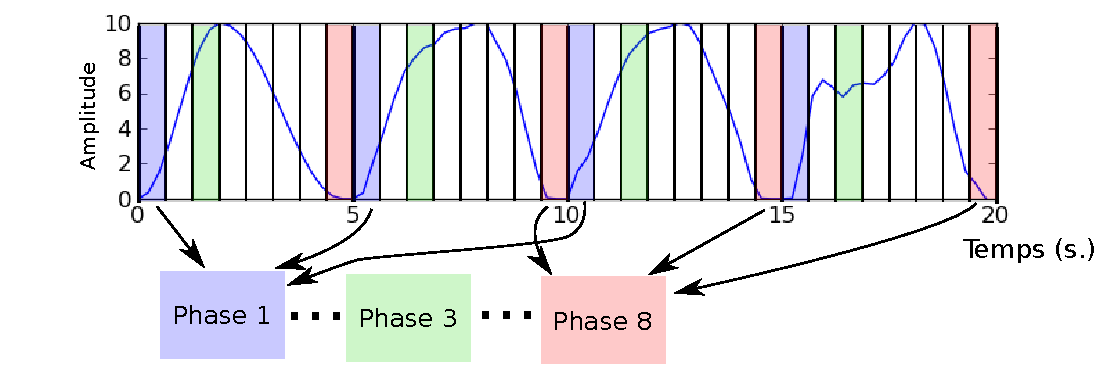
\includegraphics[width=12cm]{images/ET-IM}
	\end{center}
	\caption{Illustration de la synchronisation respiratoire en phase : Le cycle respiratoire acquis est découpé selon la position du signal acquis dans le cycle. Le signal est analysé pour déterminer les débuts et fins de cycles. Chaque cycle est découpé en un nombre déterminé de phases égales.} 
	\label{fig:gatingRespi}
\end{figure}


\begin{figure}[h!]
	\begin{center}
		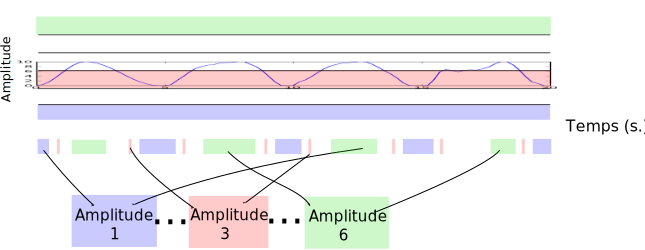
\includegraphics[width=12cm]{images/gatingAmplitude}
	\end{center}
	\caption{Illustration de la synchronisation respiratoire en amplitude : Le cycle respiratoire acquis est découpé selon son amplitude.} 
	\label{fig:gatingRespiAmplitude}
\end{figure}


Cette technique est notamment présentée dans~\cite{nehmeh2002effect}, où le signal respiratoire est estimé par une caméra qui suit un marqueur placé sur le torse du patient (système RPM de Varian Medical Systems). L'étude a été réalisée sur 5 patients volontaires comme suit : un scan de transmission de 3 minutes, suivi d'une acquisition avec correction de 10 minutes, puis d'une acquisition témoin non corrigée de 3 minutes. La décomposition du cycle s'effectue en fonction de la phase. L'auteur annonce une réduction du volume des tumeurs pouvant aller jusqu'à 34\%, avec une augmentation du $SUV_{max}$ de 160\%. 

Une autre publication~\cite{boucher2004respiratory} utilise un thermomètre détectant l'air chaud émis en début de cycle respiratoire pour réaliser la synchronisation. Les différentes reconstructions issues de l'expérience sont visibles figure \ref{fig:boucher2004}. Il faut noter que la partie clinique de cette étude a été réalisée sur 10 patients sains, et qu'il n'y a donc pas de mesures de performance de la correction du mouvement sur les lésions. 

\begin{figure}[h!]
	\begin{center}
		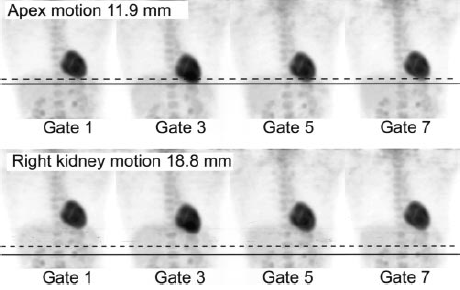
\includegraphics[width=12cm]{images/gatingBoucher2004}
	\end{center}
	\caption{Illustration de l'étendue du mouvement respiratoire sur des images reconstruites après synchronisation respiratoire~\cite{boucher2004respiratory}. La rangée du haut montre l'étendue du mouvement de l'apex du coeur, et celle du bas l'étendue du mouvement du rein} 
	\label{fig:boucher2004}
\end{figure}

Une variante de cette technique ne nécessitant pas de capteur est décrite dans~\cite{nehmeh2003reduction}. Un point faiblement radioactif est fixé au-dessus du torse du patient. Les acquisitions de l'imageur sont ensuite enregistrées par blocs temporels de 1 seconde, et une zone d'intérêt est reconstruite dans chacune des images. Les données reconstruites montrant le point source dans cette zone d'intérêt sont sommées et l'image finale reconstruite. 

Cette technique a été comparée avec celle présentée précédemment basée sur le système RPM. Ces deux techniques n'ont été testées cliniquement que sur un patient mais ont montrés des performances tout à fait semblables (6\% de différence dans les activités et 2\% pour le volume de la lésion).

Cependant ces techniques n'utilisent pas une carte d'atténuation optimisée pour la position du cycle correspondant aux acquisitions TEP.  Guoping et al.~\cite{GuopingChang2010Implementation} réalisent la carte d'atténuation à partir d'une image TDM réalisée en respiration libre synchronisée, et reconstruisent les données TEP acquises lorsque l'amplitude respiratoire est proche de celle utilisée pour l'acquisition TDM (voir exemples figure \ref{fig:chang2010}. Les résultats présentés sur 13 patients (21 tumeurs) montrent une amélioration du rapport signal sur bruit pouvant aller de -3.4 à 81\% suivant les tumeurs, avec une amélioration moyenne de 26.3\%.

\begin{figure}[h!]
	\begin{center}
		\begin{tabular}{c c}
			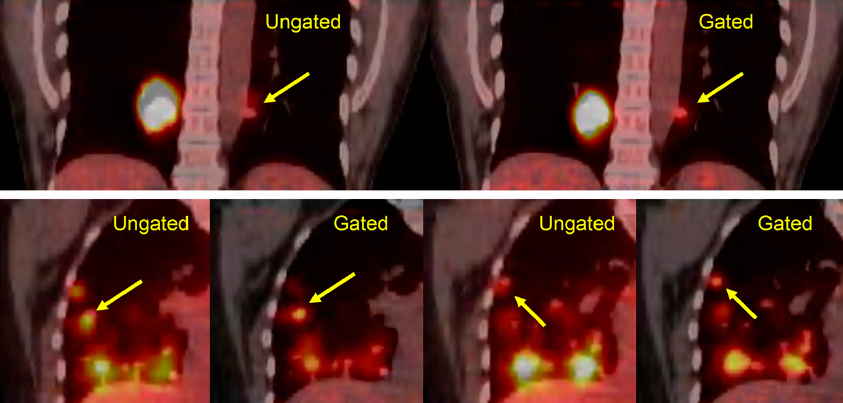
\includegraphics[width=10cm]{images/chang2010}
		\end{tabular}
	\end{center}
	\caption{Images TEP/TDM superposées du poumon reconstruites avec et sans gating respiratoire en utilisant la méthode décrite dans~\cite{GuopingChang2010Implementation}. On peut observer que les tumeurs sont mieux définies et correspondent à l'image TDM qui sert de référence.} 
	\label{fig:chang2010}
\end{figure}

Le principal problème de ces techniques est qu'elles demandent un temps d'acquisition beaucoup plus long à qualité d'image égale. Si l'on ne conserve que 20\% des évènements détectés, cela signifie qu'il faut augmenter le temps d'acquisition d'un facteur 5 pour obtenir une image d'une qualité égale. Il n'est donc pas envisageable de mettre en place ces protocoles en routine clinique, car le temps disponible n'est pas suffisant. C'est pour cela que de nombreuses équipes se sont mises à travailler sur une évolution de cette technique, où les images sont déformées les unes sur les autres pour prendre en compte toutes les informations de l'acquisition.

\section{Synchronisation respiratoire avec recalage}
\label{lab:corrPostRecon}

Dans cette section, nous allons détailler la technique consistant à corriger  le mouvement en déformant les images reconstruites.

Pour réaliser cela, les différentes techniques se basent sur une estimation préalable du mouvement respiratoire. Les images de chaque phase sont reconstruites indépendamment, puis recalées sur une phase de référence grâce au champ de mouvement. Enfin, les images déformées sont sommées. La difficulté se situe dans l'estimation du champ de mouvement interne lors de la respiration, car ce mouvement est complexe.

Les premières publications décrivant cette technique l'utilisaient notamment pour réaliser de l'imagerie cardiaque en TEP~\cite{klein19973d}. Cette publication démontre la faisabilité du procédé sur un animal en utilisant des techniques de flux optique pour estimer le champ de mouvement. En effet le coeur a l'avantage d'avoir une activité métabolique intense, ce qui rend l'estimation de son mouvement aisée même sur des images avec une faible statistique.

\subsection{Estimation du mouvement respiratoire corps entier}

L'estimation du champ de mouvement interne se fait à l'aide d'une des techniques présentées précédemment en \ref{lab:estimChamp}. Elles sont rappelées brièvement :

\subsubsection{imagerie TEP avec gating}
\label{lab:correctionDawood2008}

L`'acquisition TEP est réalisée en même temps que le signale respiratoire. Une image est reconstruite par phase du signal respiratoire, puis un algorithme d'estimation de mouvement est utilisé pour calculer le champ de mouvement entre les instants du cycle.

Les premiers algorithmes étaient utilisés en imagerie cardiaque~\cite{klein2002four} avec des transformations simples (affines), puis d'autres algorithmes plus adaptés aux images corps entier ont été utilisées, comme les flux optiques~\cite{dawood2006lung, dawood2006lung}, ou l'interpolation par B-spline~\cite{bai2009regularized}. 


\subsubsection{imagerie CT 4D}

Les images CT 4D peuvent être utilisées pour réaliser l'estimation du mouvement respiratoire au lieu des données TEP. Cela nécessite par contre une dose plus importante et un temps d'acquisition plus long.
Dawood a réalisé plusieurs publications sur le sujet en utilisant le flux optique pour l'estimation du champ de mouvement~\cite{dawood2006lung, dawood2008respiratory}. L'algorithme a été étudié sur des images de patients réels. Une autre publication~\cite{thorndyke2006reducing} indique une amélioration du rapport de contraste sur bruit (CNR) d'un facteur 3 grâce à la correction.


\section{Correction pré-reconstruction}

Les méthodes de correction du mouvement pré-reconstruction modifient les positions des Lignes de réponse (LDR) fournies par le scanner.
Ce recalage des LDR correspond à un déplacement des lignes de réponse dans l'espace du détecteur (voir fig. \ref{fig:recalageLOR}) en fonction du mouvement respiratoire. La limitation principale de ce type de méthode est que le champ de mouvement ne peut pas être élastique.

Cependant, il a été étudié en imagerie du cerveau~\cite{bloomfield2003design}, où il permettait de corriger les mouvements de la tête. Il a été aussi utilisé en imagerie cardiaque TEP~\cite{livieratos2005rigid} en utilisant un champ de mouvement rigide (rotation suivie d'une translation).

Dans les deux cas, les résultats ont montrés une nette amélioration des images (voir fig. \ref{fig:ameliorationLOR}

Dans le cadre du mouvement respiratoire du thorax, l'approche de recalage par LDR a été expérimentée par Frédéric Lamare~\cite{lamare2007respiratory}, mais avec des résultats mitigés.

\begin{figure}[h!]
	\begin{center}
		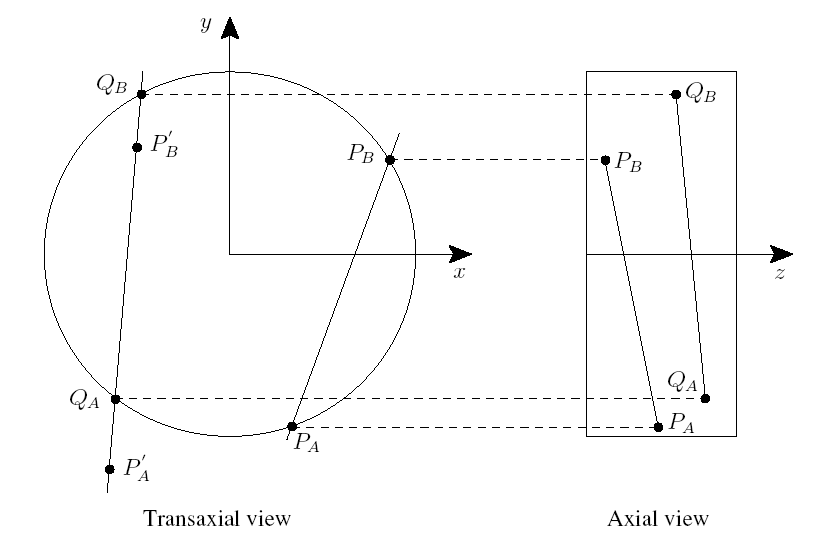
\includegraphics[width=12cm]{images/recalageLOR}
	\end{center}
	\caption{Illustration du recalage des lignes de réponse dans l'espace du détecteur : $P_A$ et $P_B$ représentent les positions des détections, $P_{A'}$ et $P_{B'}$ les positions des points corrigé et $Q_A$ et $Q_B$ les détections correspondantes } 
	\label{fig:recalageLOR}
\end{figure}

\begin{figure}[h!]
	\begin{center}
		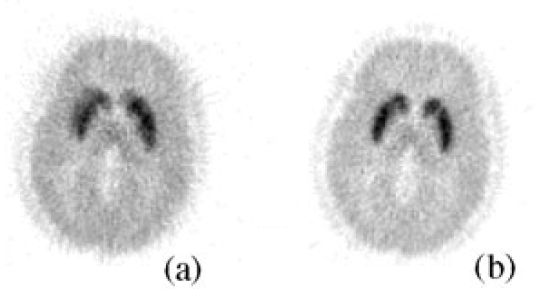
\includegraphics[width=6cm]{images/bloomfield2003design} 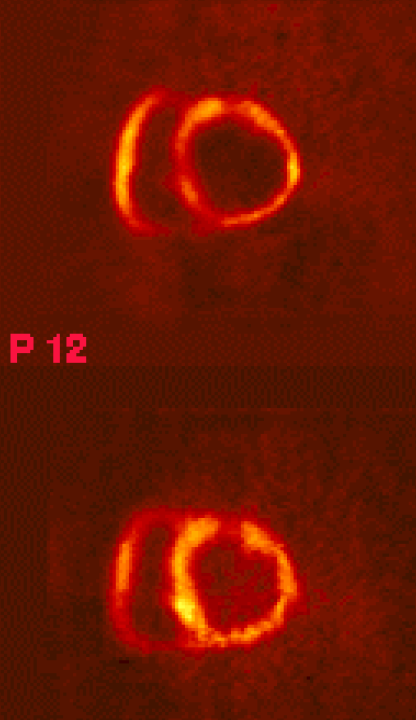
\includegraphics[width=3cm]{images/livieratos2005rigid}
	\end{center}
	\caption{Résultats de l'algorithme de recalage des LOR sur des images de patients utilisant le radio-traceur [$^{11}$C]raclopride. (a) montre une image non corrigée du mouvement et (b) une image corrigée. On peut noter que les éléments internes du cerveau sont beaucoup mieux définis. (c) représente une coupe du coeur petit axe non corrigée (en haut) et corrigée (en bas). On peut voir une amélioration de la définition de l'image.} 
	\label{fig:ameliorationLOR}
\end{figure}
 
Cette technique de correction du mouvement a été utilisée pour la correction du mouvement respiratoire du thorax~\cite{lamare2007respiratory,lamare2007list}, avec des performances plus limitées. En effet, le champ était approximé par une transformation affine, qui peut difficilement modéliser le mouvement du thorax dans son ensemble.

En effet, \cite{lamare2007respiratory} réalise une estimation du mouvement affine, en recalant les images TDM de chaque instant du cycle sur l'image de référence à l'aide d'une transformation affine par maximisation de l'information mutuelle normalisée. Le champ de mouvement  est calculé séparément pour le poumon, le coeur et trois organes sous le diaphragme (foie, estomac, rate). Les données sont des simulations réalisées par Geant4~\cite{jan2004gate} pour simuler un imageur Philips Allegro.

Ces résultats ont été améliorés par l'utilisation de la technique suivante qui permettait la prise en compte d'un mouvement élastique.

\section{Correction pendant la reconstruction}
\label{lab:CorrpendantRecon}
Plusieurs auteurs ont présentés des méthodes permettant de réaliser la correction de mouvement pendant la reconstruction. Qiao et al.\cite{qiao2006motion} et Lamare et al.~\cite{lamare2007list} ont proposé une méthode de correction du mouvement respiratoire basé sur une modification de la matrice de sensibilité lors de la reconstruction pour prendre en compte le mouvement. Tous les deux utilisent un champ de mouvement élastique estimé en utilisant un champ interpolé par B-splines.

L'algorithme original utilisé est basé sur OPL-EM~\cite{reader2002one} qui organise les données en ``sous-ensemble'' de la même manière que OS-EM~\cite{hudson1994accelerated} mais en utilisant les informations list-mode. Le principe de la reconstruction avec correction du mouvement respiratoire est décrit par la formule suivante :

\label{lab:corrMatSyst}
\begin{equation}
 f^{k+1}=\frac{f^k}{S} \sum_{t=1}^{N_{frames}} P_t^T \frac{1}{P_t f^k} 
\end{equation}

$f^k$ est l'image à l'itération $k$,

$T$ est l'opérateur de transposition

$P_t$ représente la matrice système à l'instant t. Chaque élément $p_{ij}$ de cette matrice indique la probabilité de détecter à la ligne de réponse $i$ un évènement généré au voxel $j$. 

$N$ correspond au nombre d'instants temporels considérés.

$S$ est la matrice de sensibilité :

\begin{equation}
 S=\frac{1}{N_{frames}} \sum_{t=1}^{N_{frames}} P_t^T N A_t 
\end{equation}

 $A_t$ est la matrice permettant de corriger les effets de l'atténuation au temps $t$ et $N$ est la matrice de normalisation qui compense l'inhomogénéité spatiale de la sensibilité.

Dans la publication~\cite{lamare2007list}, deux variantes de cette technique sont comparées avec la correction par synchronisation respiratoire avec recalage présentée précédemment ainsi que la correction pré-reconstruction. Les résultats présentés montrent un clair avantage pour la correction pendant la reconstruction, avec des performances couramment améliorées d'un facteur 2. 

Par exemple, la différence relative du contraste (équation \ref{eq:percentAmelioraiton}) pour une lésion de 7mm présente dans la partie haute du poumon est de 28\% pour les images non corrigées, contre 4.4\% pour les images corrigées par la méthode de correction pré-reconstruction et de 1.2\% pour la méthode de reconstruction pendant la reconstruction. De la même manière, pour des lésions de 7mm présentes dans le bas du poumon, les images non corrigées montrent une différence relative de contraste de 32\%, contre 2.63\% pour la correction pré-reconstruction et 1.66\% pour la correction pendant la reconstruction.


\begin{equation}
 \label{eq:percentAmelioraiton}
 \% Am\acute{e}lioration = \left| \frac{Image~\acute{E}valu\acute{e}e~-~R\acute{e}f\acute{e}rence}{R\acute{e}f\acute{e}rence} \right|
\end{equation}

La figure \ref{fig:lamare2007} montre un profil de l'interface poumon/foie avec une tumeur pour les différentes techniques de correction. On voit clairement que l'image non corrigée montre un retard dû au flou de mouvement. Ce retard est partiellement corrigé par la correction de mouvement pré-reconstruction, mais le profil de courbe de la méthode de correction du mouvement pendant la reconstruction est celui qui s'approche le plus de la référence.


\begin{figure}[h!]
	\begin{center}
		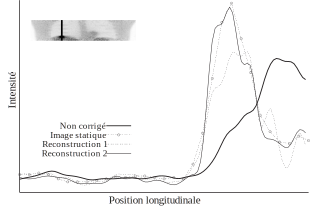
\includegraphics[width=12cm]{images/lamare2007list}
	\end{center}
	\caption{comparaison des performances des différentes techniques de correction du mouvement sur un profil d'image TEP contenant une tumeur placée au niveau du diaphragme. La référence correspond à Frame 1, LORs-Affine correspond à la correction pré-reconstruction et Elastic Method 2 corresponds à la correction pendant la reconstruction.} 
	\label{fig:lamare2007}
\end{figure}


\section{Déconvolution de l'image}

Cette technique décrite en ~\cite{naqa2006deblurring} utilise une connaissance du mouvement respiratoire acquise à partir d'une image TDM 4D pour déduire un filtrage appelé TLP (\textit{Tumor Location Probability}) qui correspond à la dégradation dû au mouvement respiratoire.

L'image est ensuite déconvoluée pour corriger les effets du mouvement respiratoire. Cette méthode a été évaluée sur un fantôme physique et des patients réels à l'aide d'un grand nombre de critères provenant pour partie de la TEP (sous-estimation de l'activité de la tumeur, exemples d'images), et pour partie du domaine de la déconvolution (entropie, ``rugosité'').

Les résultats présentés en \ref{fig:performanceDeconvolution} montrent une nette amélioration des performances sur des fantômes, pour un déplacement axial simple de 20mm. L'activité des lésions de fort diamètre est correctement récupérée quelque soit l'algorithme utilisée, mais il n'a pratiquement pas d'effets sur les lésions de 1cm de diamètre.

Ce type d'algorithme est peu présenté dans la littérature. 

\begin{figure}[h!]
	\begin{center}
		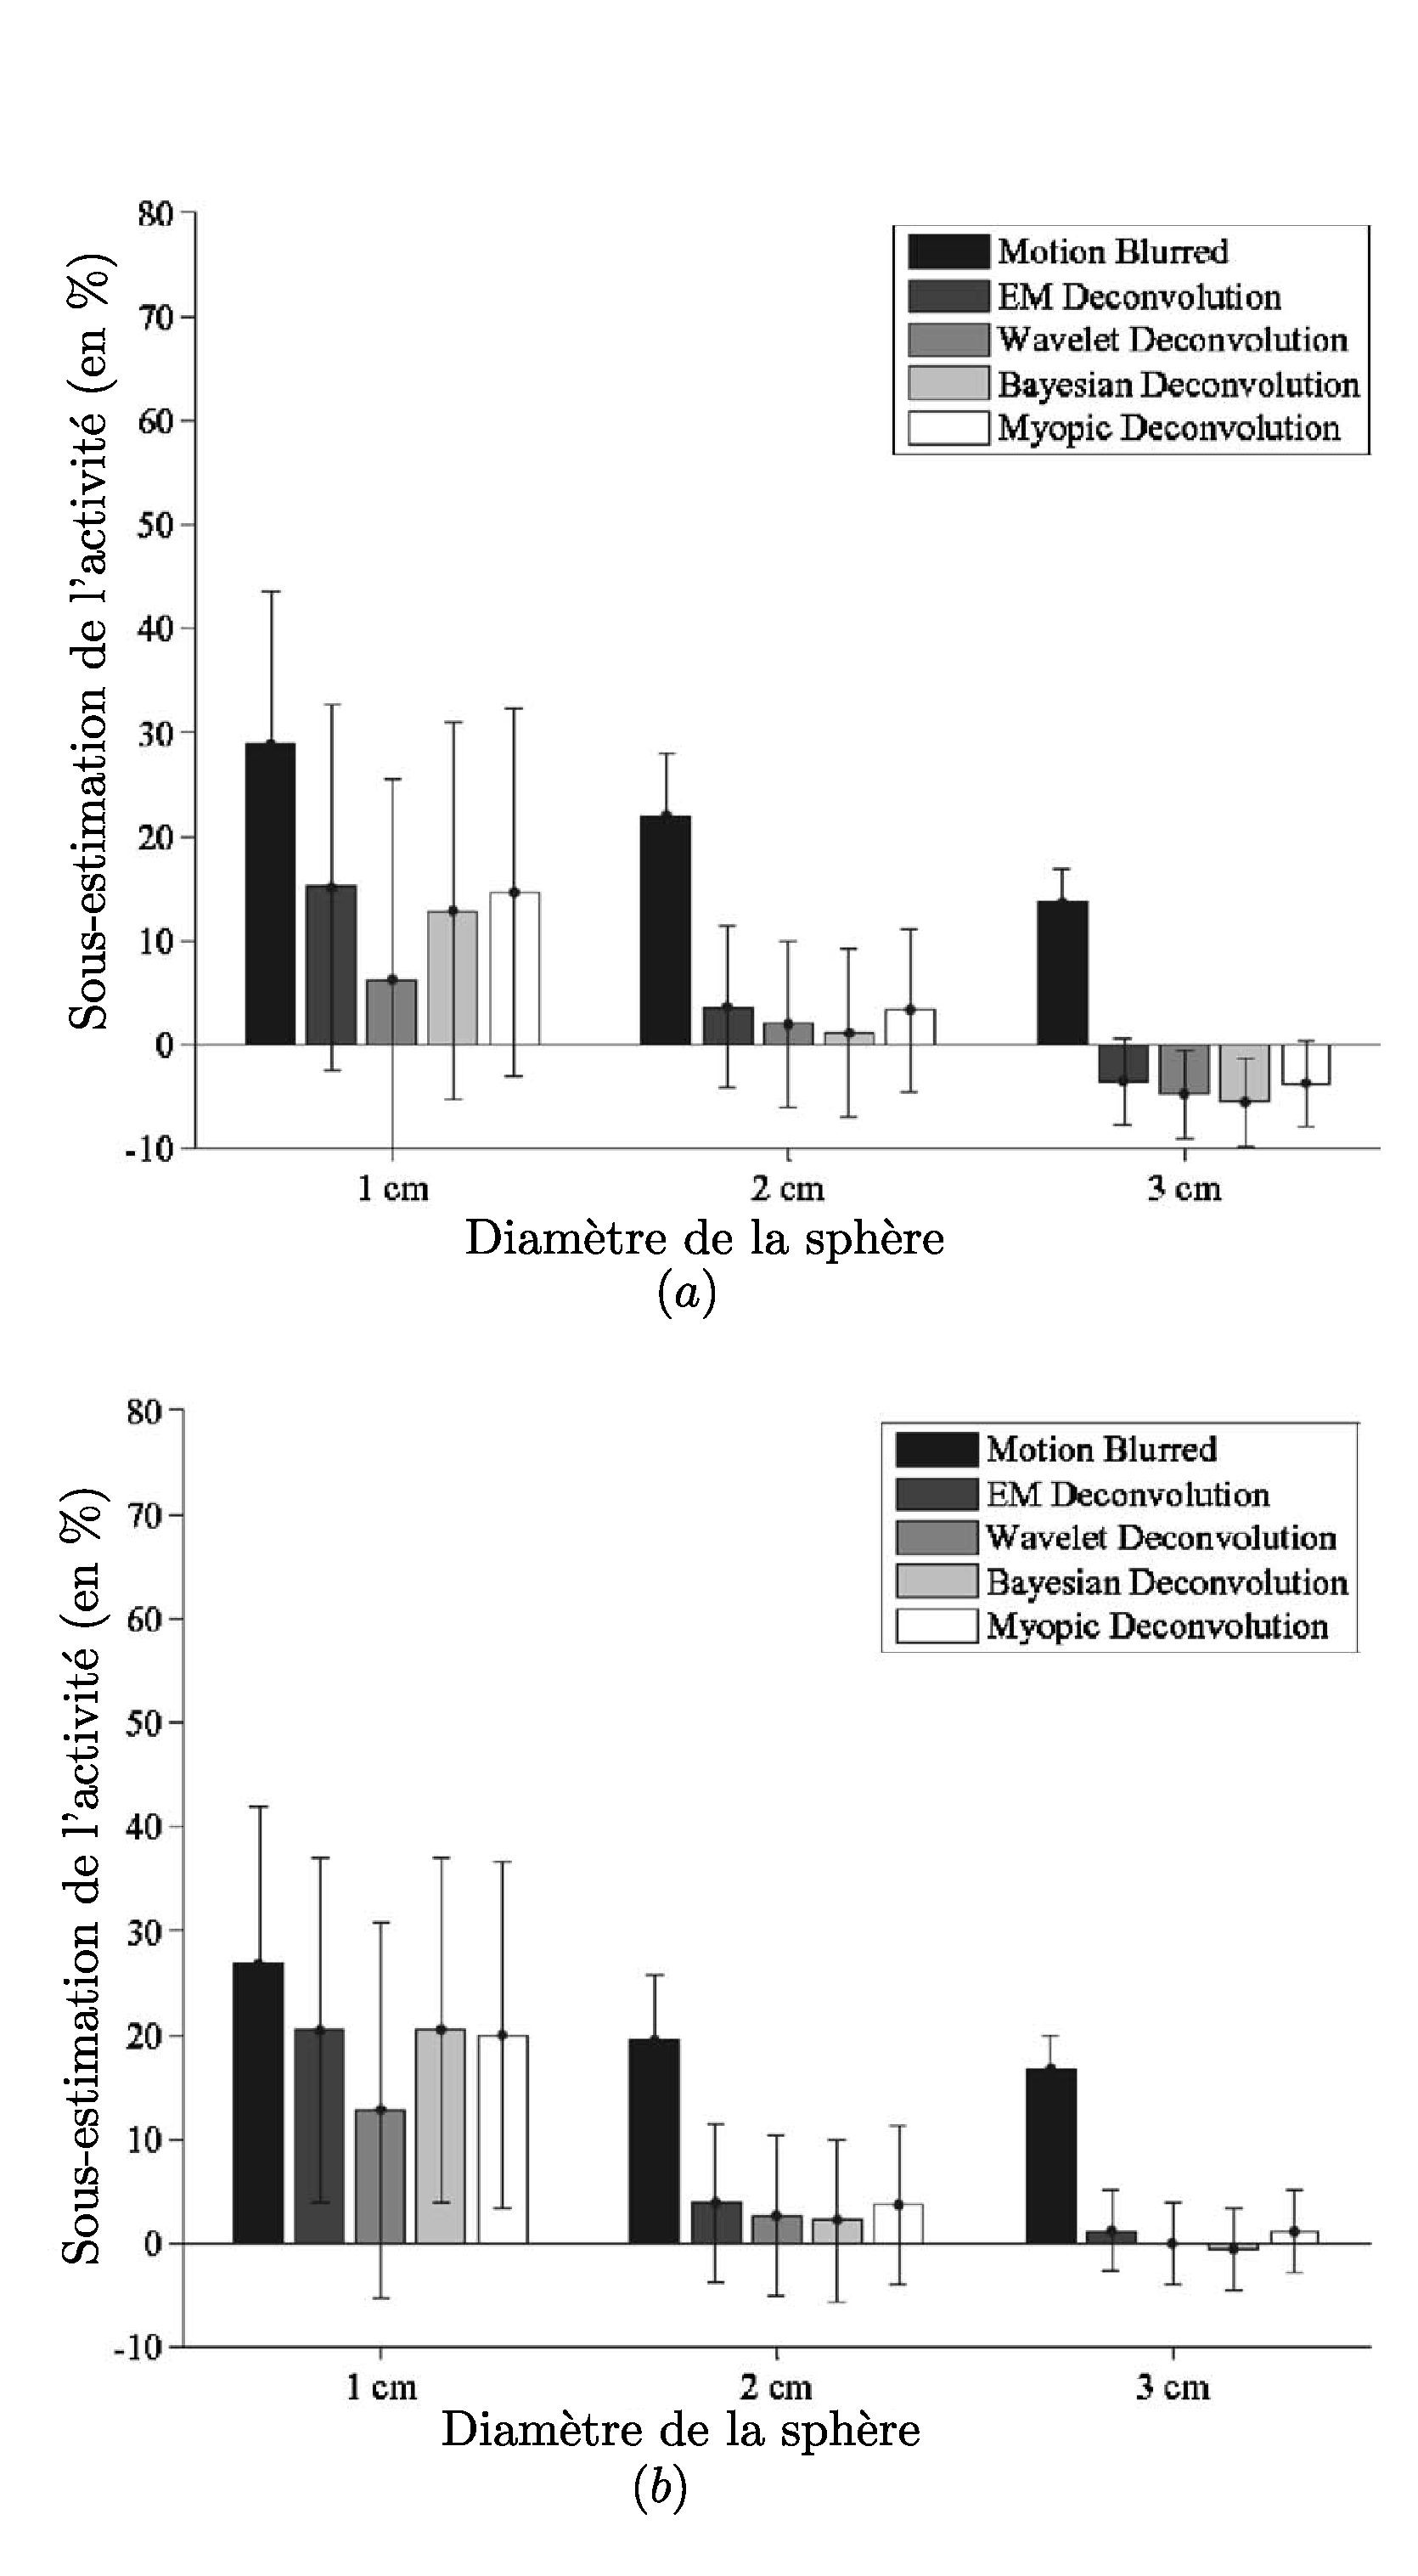
\includegraphics[width=10cm]{images/performanceDeconvolution}
	\end{center}
	\caption{Comparaison de l'erreur de sous-estimation de l'activité des lésions en fonction de l'algorithme de déconvolution utilisé sur des fantômes. En a) la lésion a une activité moyenne, tandis qu'en b) l'activité de la lésion est faible par rapport au fond. Le déplacement de la lésion est le même dans les deux cas (2cm)} 
	\label{fig:performanceDeconvolution}
\end{figure}


Un autre article utilisant aussi des algorithmes de déconvolution a été présenté par wiemker~\cite{wiemker2008combined}. Cependant il ne cherche pas à corriger le mouvement respiratoire sur l'ensemble de l'image mais principalement à améliorer la mesure du SUV sur une lésion. Pour cela, il réalise une estimation de la fonction d'étalement du point (FEP) de l'imageur TEP au niveau de la lésion à l'aide d'un contourage de la lésion réalisé préalablement dur une image TDM. L'estimation de la FEP permet de prendre en compte à la fois les effets du mouvement respiratoire et ceux de la FEP intrinsèque à l'imageur TEP. 

Cependant, cette technique est inapplicable dans notre cas car les lésions doivent être suffisamment importantes et homogènes pour pouvoir les délimiter de manière fiable sur les images TDM, ce qui n'est pas notre cas.


\part{Evaluation des performances de détection}
	\chapter{Performance des outils de détection}
\label{lab:chapCAD}
	\section{Généralités}

En oncologie, la détection des sites tumoraux est une étape capitale dans la prise en charge des patients. 
Dans cette partie, je vais détailler les techniques qui permettent de comparer les performances de plusieurs observateurs (médecins ou algorithmes) face aux mêmes images, ou alors du même observateur face à plusieurs types d'images différentes.

Pour cette section, le problème va être simplifié au cas où un observateur doit classer un signal en ``Sain'' (normal, HO) ou ``Pathologique'' (anormal, H1). 

Les performances de l'observateur sont indiquées par la matrice de confusion (table~\ref{tab:confusion}), qui recense les signaux correctement et incorrectement classés.

\begin{table}[h]
	\label{tab:confusion}
	\begin{tabular}{cc c|c|}
		& & \multicolumn{2}{c}{Classe estimée} \\
		\cline{3-4}	
		& & \multicolumn{1}{|c|}{Sain} & Pathologique \\ 
		\cline{2-4}
		\multicolumn{1}{c|}{\multirow{2}{*}{Classe réelle}} & \multicolumn{1}{|c|}{Sain} & VN (\emph{Vrai Négatif}) & FP (\emph{Faux Positif})\\
		\cline{2-4}
		\multicolumn{1}{c|}{} & \multicolumn{1}{|c|}{Pathologique} & FN (\emph{Faux Négatif}) & VP (\emph{Vrai Positif})\\
		\cline{2-4}
	\end{tabular}
	\caption[Matrice de confusion]{Matrice de confusion : donne une vue
d'ensemble des performances du classifieur. Elle indique le résultat de la
classification de signaux connus.}
\end{table}

On utilise habituellement deux grandeurs pour mesurer les performances de l'observateur :

La \emph{sensibilité} (voir l'équation~\ref{eq:sensib}) correspond à la proportion d'images correctement évaluées pathologiques par l'observateur par rapport au nombre total d'images réellement pathologiques. Elle donne une information sur la capacité de l'observateur à détecter les cas pathologiques.
\label{lab:pressensib}
\begin{equation}
	\label{eq:sensib}
	Sensibilit\acute{e} = \frac{VP}{VP + FN}
\end{equation}

La \emph{spécificité} (voir équation~\ref{eq:specif}) représente le même type de grandeur, mais cette-fois ci appliquée aux cas non pathologiques : elle correspond à la capacité de l'observateur à donner un résultat négatif lorsque l'image est non pathologique.

\begin{equation}
	\label{eq:specif}
	Sp\acute{e}cificit\acute{e} = \frac{VN}{VN + FP}
\end{equation}

Ces deux grandeurs sont complémentaires mais ne permettent pas à elle seules de comparer les performances de différents observateurs. En effet, un  utilisateur va souvent donner des notes, qui vont indiquer son niveau de confiance sur la présence de la pathologie (à ne pas confondre avec des notations sur la gravité des lésions, comme les techniques de gradation de~\cite{genestie1998comparison}).

Les techniques de comparaison de systèmes de décision comme l'analyse ROC (Receiver-Operating Curve) permettent de prendre en compte ces incertitudes. Elles proviennent à l'origine du domaine des télécommunications pendant la seconde guerre mondiale, où il fallait une métrique permettant de tester les performances des systèmes RADAR~\cite{zou2007receiver} pour la détection des avions ennemis. Les courbes ROC servent donc à évaluer la capacité d'un ou plusieurs ``observateurs'' à discriminer des signaux entre deux classes ``normal'' et ``anormal''. Les informations de sensibilité et de spécificité se limitent à comparer les performances pour un niveau de confiance donné.

\subsection{Définition d'un Vrai positif / Faux positif}

En général, les systèmes CAD, que nous présentons dans le chapitre 8 génèrent des cartes paramétriques, sur lesquels les voxels ou des groupements de voxels reçoivent une valeur correspondant à leur classe. 

Afin de déterminer si l'élément (voxel ou groupement de voxels) noté ``anormal'' fait effectivement partie d'une lésion, sa  position est généralement comparée à celle des lésions de la vérité terrain. Une distance d'acceptation est utilisée pour prendre en compte une éventuelle imprécision du système CAD. Par exemple, l'auteur de~\cite{paik2004surface} considère que l'élément est un vrai positif si il est contenu dans le volume de la tumeur de la vérité terrain.

Cependant, il existe plusieurs stratégies pour compter les FP :
\begin{itemize}
 \item Par voxel ou groupe de voxel (3D).
 \item Par coupe (2D).
\end{itemize}

Ces deux techniques vont très fortement influer sur le nombre de faux positifs pour le même système CAD. En effet, dans le cas où le comptage des FP est réalisé sur l'ensemble de l'image, chaque groupement ou voxel ne correspondant pas à une lésion est noté FP. L'auteur de~\cite{paik2004surface} indique par exemple 165 faux positifs par images TDM pour une sensibilité de 100\%. De même,~\cite{zhao2003automatic} montre une sensibilité de 94\% avec 906 faux positifs par image TDM pour la détection du cancer du poumon. Ces résultats montrent des nombre de faux positifs très importants, mais ne peuvent pas être comparés avec ceux utilisant un chiffrage des FP par coupe. En effet, dans ce cas, ``FP'' correspond au nombre de coupes contenant au moins un élément n'étant pas une tumeur. Le nombre de faux positifs est donc borné par le nombre de coupes, et ne fait pas de différences entre des coupes contenant un grand nombre de lésions et celles n'en contenant qu'une. 

\textbf{Dans le reste du document, nous considèrerons le premier système de comptage des FP : tout élément du volume à observer n'étant pas en contact avec une tumeur sera compté comme un faux positif.}


	\section{Méthodologie ROC - Receiver-Operating Curve}

Les courbes ROC~\cite{swets1982evaluation,metz1986roc} sont des courbes indiquant la spécificité et la sensibilité de l'observateur (humain ou numérique) pour différents niveaux de certitude. Elles fournissent une mesure objective des performances d'un observateur dans une tâche de discrimination entre deux classes. 

Elles peuvent être utilisées pour comparer les performances relatives de différents observateurs avec la même modalité d'imagerie ou pour déterminer les paramètres optimaux de ces images. L’évaluation d'un observateur par la méthode ROC nécessite la création d'un jeu de données labellisées en deux classes : Normale (H0) et Pathologiques (H1). L'observateur va se voir présenter l'ensemble des images et devra les noter individuellement selon un barème défini à l'avance (par exemple 0: définitivement normal, 1: potentiellement normal, 2: équivoque, 3: potentiellement pathologique, 4: définitivement pathologique). Par convention, plus la note (notée $\lambda$) sera élevée, plus l'observateur va considérer qu'il est en présence d'un cas pathologique. A l'inverse, une note basse va indiquer un cas présumé sain ou normal. 


\begin{figure}[h]
	\begin{center}
	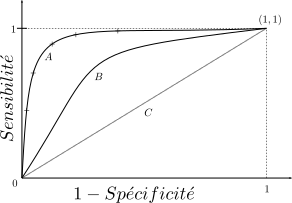
\includegraphics[width=10cm]{images/illustrationROC}
%	\vspace{-0.5cm} % Ugly Moche Hideux
	\end{center}
	\caption[Exemple de courbe ROC]{Exemple de courbe ROC. La courbe $A$ représente le résultat d'une évaluation ROC avec un barème à 6 niveaux. Pour chaque note du barème, le point correspondant est affiché en reportant la spécificité et la sensibilité (représentés par les croix). La courbe $B$ représente une autre évaluation, avec des performances inférieures : Pour chaque niveau de ``1-Spécificité'', la sensibilité de la courbe $B$ est inférieure à celle de la courbe $A$. Le courbe $C$ représente le d'un classifieur qui donne ses réponses de manière aléatoire.}
	\label{fig:illustrationROC}
\end{figure}

L'observateur peut être un humain ou un algorithme, et les notes peuvent être discrètes ou continues. 

Le tracé de la courbe ROC se fait en reportant la sensibilité et la valeur "1-spécificité" du classifieur pour différents seuils de décision. Par construction, la courbe va commencer au point $(0,0)$ (tous les points sont diagnostiqués négatifs) et se terminer au point de coordonnée $(1,1)$ (tous les points sont diagnostiqués positifs). Deux exemples de courbes ROC sont présentés sur la figure~\ref{fig:illustrationROC}.


Pour analyser les courbes ROC, on considère que les distributions de probabilité des notes des cas H0 et H1 suivent une loi gaussienne (voir figure~\ref{fig:loiROC}). Ce modèle de décision suppose que l'ensemble des valeurs de $\lambda$ évaluées sur des cas H0 (sain) suit une distribution de probabilité $P(\lambda_0, \sigma_0)$ de valeur moyenne $\lambda_0$ et d'écart-type $\sigma_0$. De même, les valeurs de $\lambda$ évaluées sur des cas H1 (pathologiques), suivent une distribution de probabilité $P(\lambda_1, \sigma_1)$. Le mécanisme de décision se base sur le choix d'une valeur de seuil $\lambda_s$ au-delà de laquelle les observations sont considérées comme pathologiques.

Ce seuil permet de modifier de manière dynamique la répartition des observations dans la matrice de confusion.  Cela permet d'enrichir la comparaison des observateurs par rapport au couple (sensibilité/spécificité) seul.

Selon cette hypothèse gaussienne, on peut montrer que la distance $d$, appelée indice de détectabilité, correspond à l'aire sous la courbe ROC :


\begin{equation}
 d= \frac{\lambda_1 - \lambda_0}{\sqrt{\sigma_1 + \sigma_0}}
\end{equation}

\begin{figure}[h]
	\begin{center}
	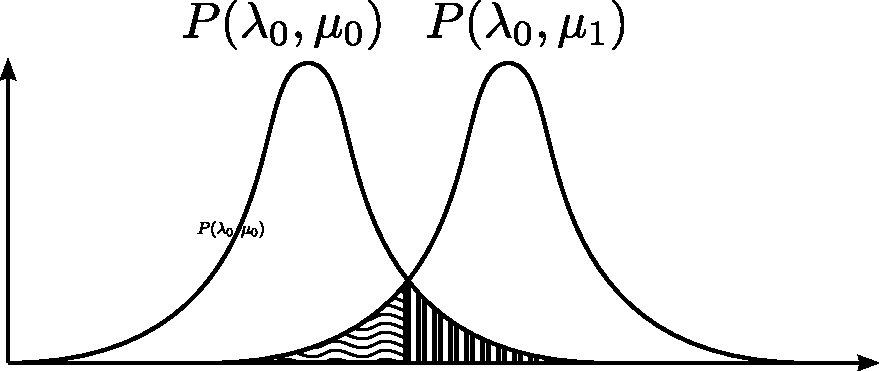
\includegraphics[width=10cm]{images/loiROC}
	\vspace{-0.5cm} % Ugly Moche Hideux
	\end{center}
	\caption[Modèle de la distribution de probabilité de la variable de décision]{Modèle de la distribution de probabilité de la variable de décision dans pour les populations H0 ($P(\lambda_0, \mu_0)$) et H1 ($P(\lambda_1, \mu_1)$) dans les études ROC. $\lambda_s$ représente le seuil à partir duquel une observation sera catégorisée H0 ou H1.}
	\label{fig:loiROC}
\end{figure}




Un ensemble d'indicateurs et de figures de mérite (FDM) permettent de comparer les performances de détection à partir des courbes ROC. La FDM la plus simple consiste à choisir un niveau de spécificité (noté $\alpha$) et à comparer les sensibilités des différents observateurs. L'avantage de ce système est qu'il permet de comparer les performances dans des conditions proches de la réalité, où l'on cherche à rester dans un taux de spécificité donné. Cependant, les résultats vont dépendre du paramètre $\alpha$. Une métrique plus globale est l'aire sous la courbe ROC. \'Etant donné que la courbe est nécessairement comprise dans un carré unitaire, la valeur de l'aire sera comprise entre 0 (le classifieur donne systématiquement les mauvaises réponses), 0.5 (le classifieur donne des réponses aléatoires) et 1 (le classifieur donne toujours la bonne réponse)~\cite{nie2006integrating}.

Il est important, lors du calcul de la FDM, d'avoir une estimation de l'erreur. Il est possible de l'estimer en ajustant une courbe théorique (répondant à la loi théorique de la figure~\ref{fig:loiROC}). Plusieurs logiciels ont été développés pour estimer les paramètres, qui ont été comparés dans la publication~\cite{CarstenStephan03012003} (AccuROC, Analyse-It, CMDT, GraphROC, MedCalc, mROC, ROCKIT, and SPSS).

\label{lab:p-valeur}
Une grandeur souvent utilisée dans la littérature pour évaluer la pertinence d'un résultat est la \emph{p-valeur}. Elle représente la probabilité d'obtenir des différences entre deux courbes au moins aussi extrême que la différence observée (dans notre cas, les courbes ROC), en prenant en compte l'hypothèse selon laquelle le classifieur est aléatoire. Elle permet de vérifier si le test est statistiquement significatif.

Le problème de la méthodologie ROC est que l'observateur ne donne pas d'information de localisation de la pathologie dans l'image. On lui présente une image et il doit la noter sans indiquer la localisation de la zone suspecte. Dans notre cas, nous voulons comparer des observateurs qui réalisent une tâche de détection et de localisation de la zone suspecte. Il faut non seulement savoir si des lésions sont présentes, mais aussi avoir leur nombre et leur localisation. Cela est proche du travail en routine clinique, qui consiste à évaluer l'étendue et le nombre des lésions pour déterminer l'efficacité d'un traitement par exemple. 

Pour éviter cette limitation, plusieurs extensions à la méthodologie ROC sont décrites dans la littérature : L-ROC, AF-ROC ou encore F-ROC. Les L-ROC sont décrites ci-après, tandis que les AF-ROC et F-ROC seront décrites dans la section suivante.

\subsection{Courbes ``Localization ROC'' (L-ROC)}

L'analyse L-ROC~\cite{farquhar1999roc} ajoute l'information de localisation lors de la décision. L'observateur doit indiquer sur l'image qu'il considère comme pathologique la localisation de la lésion la plus probable. Elle est considérée comme un vrai positif si la distance entre la localisation indiquée et la localisation réelle de la lésion est inférieure à une certaine distance.

Cependant, bien que cette technique prenne en compte l'information de localisation, elle ne permet pas de traiter de manière satisfaisante les cas de lésions multiples.


\section{Courbes Free ROC}	

Les courbes Free-ROC permettent de prendre en compte plus d'informations que les courbes vues précédemment car elles utilisent non seulement les informations de localisation, mais prennent aussi en compte le concept de faux positifs de manière plus approfondie, avec la possibilité d'avoir à la fois des faux positifs et des vrais positifs dans une même image.

\subsection{Courbes Free-ROC}
\label{lab:FROC}

Les courbes F-ROC~\cite{bunch1978free} sont une généralisation des courbes ROC aux cas où l'on évalue la capacité de l'observateur à détecter un ensemble de lésions dans une série d'images. Chaque image pouvant contenir un nombre indéfini de lésions. L'observateur va donc devoir pointer sur l'image l'ensemble des sites suspects et y associer une note.

Dans ce cas, on ne peut pas utiliser le formalisme ROC car le terme de spécificité n'est pas directement calculable pour chaque niveau de confiance. On utilise à sa place le nombre moyen de faux positifs par image pour un seuil donné (voir figure~\ref{fig:courbeFROC}).

On utilise les termes de LL (Lésion localisée) et NL (Non-Lésion) en lieu et place des informations de vrai positifs et faux positifs sur les courbes ROC. De la même manière, la sensibilité et la spécificité sont respectivement FLL (Fraction de lésions correctement détectées et localisées) et NFM (Nombre de faux positifs moyens par image).


\begin{figure}[h]
	\begin{center}
	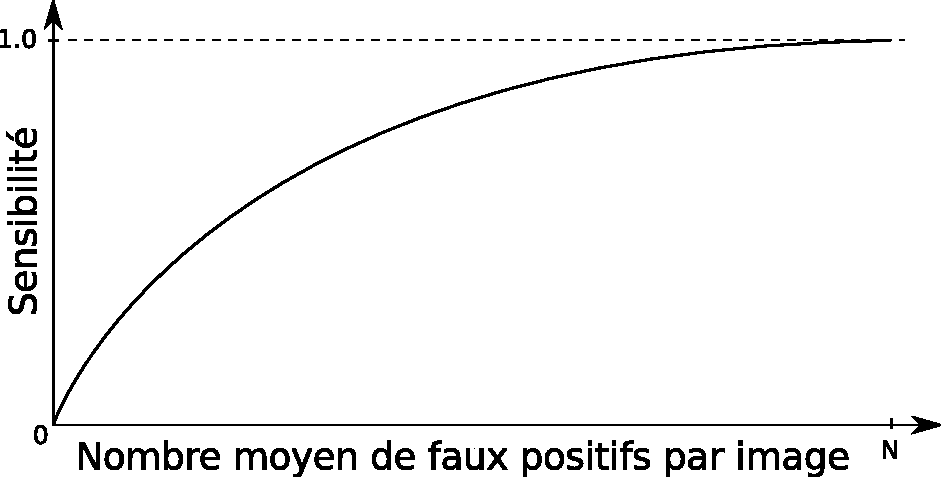
\includegraphics[width=15cm]{images/FROC}
	\end{center}
	\caption{Exemple de courbe Free ROC}
	\label{fig:courbeFROC}
\end{figure}

Les courbes F-ROC n'ayant pas de bornes sur l’axe des abscisses, il est impossible de comparer plusieurs courbes à partir de l'aire sous la courbe. Il reste cependant possible de comparer la sensibilité pour un nombre de faux positifs donnés, mais on retrouve les mêmes problèmes que pour l'analyse ROC : il faut choisir un paramètre.

\subsection{Courbes Alternative Free-ROC}

Les courbes A-FROC~\cite{chakraborty1990free} sont des extensions des courbes Free-ROC présentées précédemment mais qui ne prennent en compte que le faux positif de plus haut score par image, ce qui ne pénalise pas le cas où un observateur indique un grand nombre de fausses détections (NL). On se retrouve alors dans la situation de courbes bornées sur l'axe des abscisses, ce qui permet leur comparaison.

\subsection{Comparaison des courbes}
\label{lab:AFROC}
Plusieurs techniques ont été développées pour permettre de réaliser des comparaisons de courbes dérivées de la méthodologie F-ROC. De la même manière que pour les courbes ROC, il est possible de comparer les courbes F-ROC en fonction de la FLL pour un nombre de faux positifs donnés. Cependant, étant donné que les courbes F-ROC n'ont pas de fin déterminée, il n'est pas possible d'utiliser l'aire sous la courbe. 

JAFROC~\cite{chakraborty2004observer} (JAcknife Free Receiver Operating Curve) est un algorithme et un logiciel développé par Chakraborty et se base sur une FDM non liée directement à la courbe. Cette mesure de performance utilise un algorithme dérivé des études A-FROC, ce qui signifie qu'il n'utilise pas l'ensemble des informations disponibles dans les courbes F-ROC mais se borne à comparer les scores des faux positifs de plus forte note pour chaque image avec les notes des vrais positifs. La figure de mérite $\theta_J$ proposée mesure la probabilité d'avoir un score de vrai positif supérieur à celui d'un faux positif (de n'importe quelle image).

Soit $\theta_J$ la valeur de la FDM, $N_T$ le nombre total d'images, indexées par $i$, $N_A$ le nombre total de cas pathologiques, indexées par $j$. $n_j$ est le nombre total de lésions dans le cas anormal $j$.

\begin{equation}
\label{eq:JAFROC1}
\begin{array}{l}
	\displaystyle \theta_J=\frac{1}{N_T N_A} \sum_{i=1}^{N_T} \sum_{j=1}^{N_A} \sum_{k=1}^{n_j} W_{jk} \psi(X_i, Y_{jk}) \\
	\\
	\displaystyle \psi(X,Y) = \left\{
		\begin{array}{lll}
			1.0 & \mbox{si} & Y > X \\
			0.5 & \mbox{si} & Y = X    \\
			0.0 & \mbox{si} & Y < X    \\
		\end{array}
	\right. \\
	\\
	\displaystyle \mbox{avec} \sum_{k=1}^{n_j} W_{jk} = 1 \\
\end{array}
\end{equation}

$X_i$ le score du plus haut faux positif de l'image $i$, $Y_{jk}$ est la note de la lésion k de l'image j. Si une lésion n'a pas été détectée, alors sa note sera par défaut de "0".

Les poids $W_{jk}$ correspondent à l'importance relative de détecter la lésion $k$ dans l'image $j$ pour le diagnostic. Pour chaque image, la somme des poids doit être égale à 1.

Une seconde version de JAFROC existe avec une puissance statistique plus importante, mais elle nécessite de disposer d'un grand nombre de cas non pathologiques. La formule est la même que la précédente (équation~\ref{eq:JAFROC1}). La seule différence est que la première sommation se fait sur l'ensemble des cas non pathologiques $N_N$ (équation~\ref{eq:JAFROC2}) au lieu de l'ensemble des cas $N_T$.

\begin{equation}
\label{eq:JAFROC2}
\theta_J=\frac{1}{N_T N_A} \sum_{i=1}^{N_N} \sum_{j=1}^{N_A} \sum_{k=1}^{n_j} W_{jk} \psi(X_i, Y_{jk})
\end{equation}


\chapter{Systèmes de détection}

\section{Principe des CAD}

\subsection{Introduction}

Les systèmes CAD (Computer-Aided-Detection) sont des algorithmes permettant d'assister le praticien dans la détection des lésions ou le classement des images médicales. Dans le cadre de l'imagerie TEP oncologique, le besoin principal est celui du suivi thérapeutique, pour lequel, il est important de détecter d'éventuelles lésions résiduelles. Pour cela, il faut que le système CAD soit particulièrement adapté à la recherche de petites lésions de faible contraste qui pourraient échapper au médecin. Cependant, le diagnostic, qui consiste à évaluer la dangerosité des lésions, et leur caractère pathologique est une tâche plus complexe qui relève plus des systèmes d'aide au diagnostic, qui ne seront pas traités ici.

Le développement des systèmes CAD a débuté dans les années 1980~\cite{chan1987image}, notamment pour détecter les micro-calcifications en mammographie. Bien qu'il existe plusieurs systèmes CAD commerciaux pour l'imagerie TDM (xLNA pour Philips par exemple), aucun CAD commercial pour la TEP n'existe à notre connaissance.

\'Etant donné que les systèmes d’aide à la détection dédiées à l’imagerie TEP restent limitées,  le travail de cette thèse s’est largement inspiré de la méthodologie suivie lors du développement de systèmes CAD dans d’autres modalités d’imagerie médicale et particulièrement la mammographie et l’imagerie TDM. La classification supervisée permet de profiter de la disponibilité \textit{a priori} d’images préalablement classées pour fournir un ‘superviseur’ efficace et paramétrable. Le paragraphe suivant définit les différentes étapes standardisées d’un système CAD supervisé.


\subsection{Les différentes étapes d’un système CAD supervisé}

Comme rappelé dans la publication~\cite{li2007recent}, un système CAD est constitué de deux étapes majeures : l’identification initiale des tumeurs et la réduction de faux positifs. 

L’objectif de l’identification initiale des tumeurs (figure \ref{fig:presSystemesCAD}.1),2) et 3)) est de localiser les structures potentiellement suspectes de l’image avec la plus grande sensibilité possible au coût d’un grand nombre de fausses détections. Différents choix méthodologiques doivent être précisés pour cette étape :


\begin{figure}[h]
	\begin{center}
	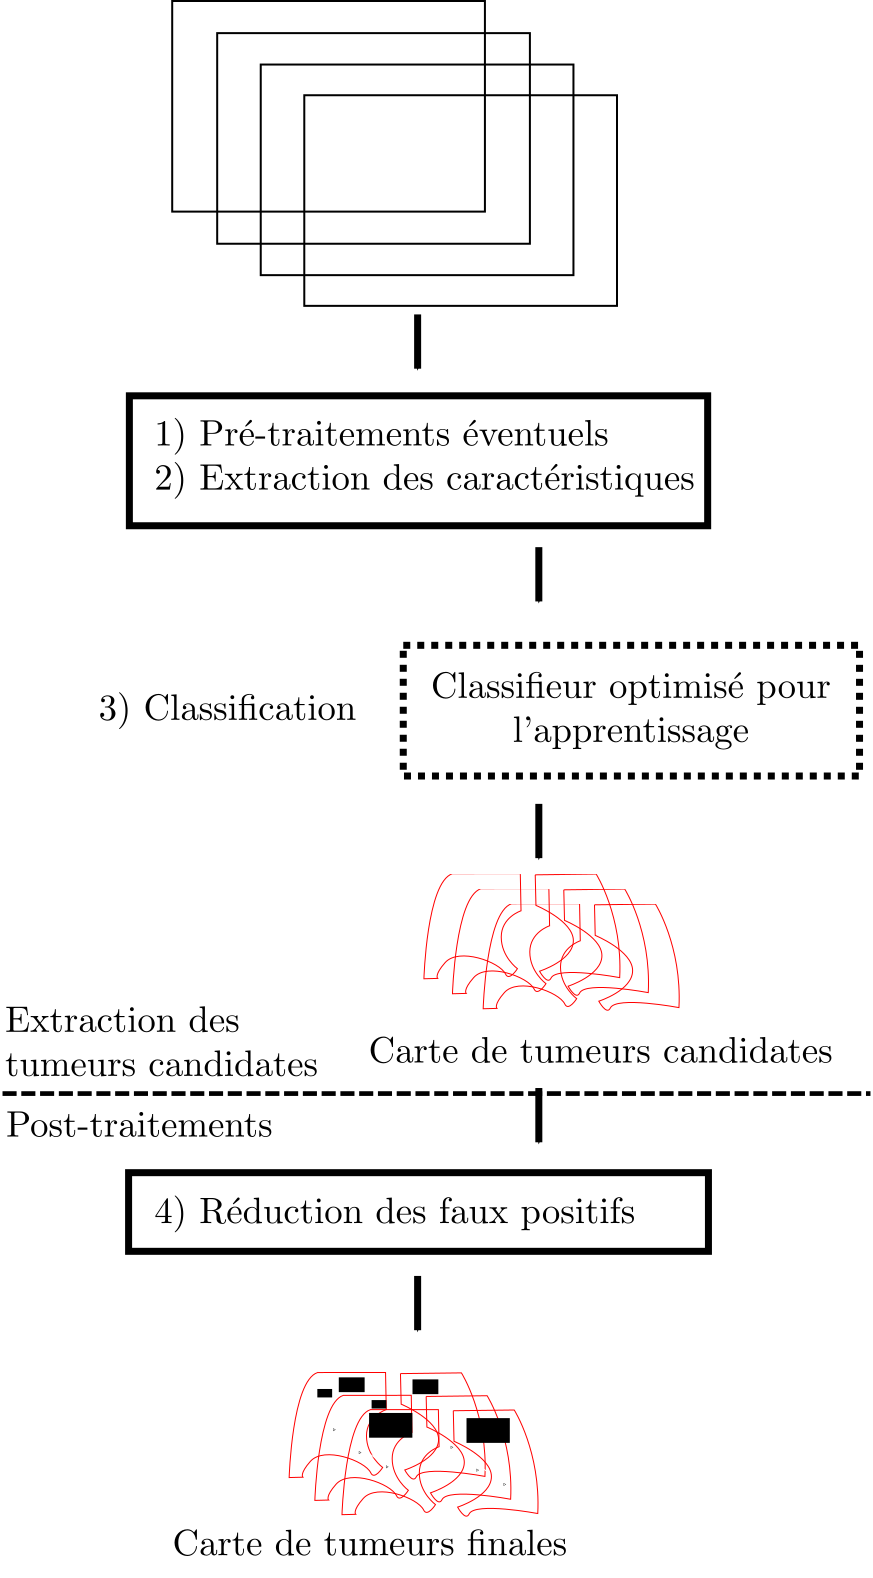
\includegraphics[width=12cm]{images/principeCAD}
	\end{center}
	\caption{Les différentes étapes d'un système CAD.}
	\label{fig:presSystemesCAD}
\end{figure}


\begin{itemize}
\item Les régions ou organes d’intérêt du système, lorsque celui-ci n’est pas dédié au corps entier, peuvent être séparés. L’image ou les régions d’intérêt de l’image peuvent ensuite être améliorées lors d’une étape de prétraitement, reposant par exemple sur du rehaussement du contraste ou du débruitage (figure \ref{fig:presSystemesCAD}.1) ).
\item Le processus d’extraction des tumeurs suspectes passe ensuite par l’utilisation d’un système de classification (figure \ref{fig:presSystemesCAD}.3) )., optimisé par un apprentissage, s’appliquant sur un ensemble de caractéristiques de l’image ou de la structure cible (figure \ref{fig:presSystemesCAD}.2) ). Ce dernier a pour but de déterminer la classe, « tumeur présente » ou « tumeur absente », de l’image ou de la structure cible. 
\end{itemize}
L’objectif de l’étape de réduction de faux positifs (figure \ref{fig:presSystemesCAD}.4) ) est de fortement réduire les fausses détections extraites de l’étape précédente, tout en conservant une sensibilité élevée. Cette étape rassemble un ensemble de méthodes permettant de trier les tumeurs candidates précédemment extraites afin de ne conserver que les candidats les plus ‘suspects’.  

	\section{Les CAD en TEP}
\label{lab:CADTEP}

Quelques systèmes CAD sur des images TEP ont été décrits dans des travaux académiques, tels que~\cite{guan2006automatic}, qui recherche des anomalies dans le corps entier. Cependant, ils ne donnent pas de mesures de performances quantitatives. La publication de~\cite{kanakatte2008pulmonary} utilise des systèmes de classification supervisés (K plus proches voisins et SVM décrits en~\ref{lab:SVM}). Un seuillage est réalisé, puis les candidats sont classés en utilisant des caractéristiques fréquentielles et les moments statistiques. 

Certaines publications utilisent seulement l'imagerie fonctionnelle TEP~\cite{ying2004novel, kanakatte2007pilot, kanakatte2008pulmonary, saradhi2009framework, el2009exploring, mhd2010artificial}, tandis que d'autres combinent cette information avec l'imagerie TDM~\cite{jafar2006computerized, nie2006integrating, potesil2007automated}.

La plupart des travaux réalisés dans le domaine ont portés sur la segmentation de lésions présélectionnées pour réaliser de l'estimation de volume pour de la planification de radiothérapie ou du suivi thérapeutique~\cite{kanakatte2007pilot, potesil2007automated, kanakatte2008pulmonary, yu2009automated}. Des publications récentes se sont focalisées sur la problématique du diagnostic pour la classification de nodules~\cite{nie2006integrating} ou la prédiction d'évolution des lésions suite à un traitement~\cite{el2009exploring}. Cependant, très peu d'études se sont focalisées sur la problématique de la localisation des lésions~\cite{guan2006automatic, kanakatte2007pilot, kanakatte2008pulmonary, mhd2010artificial}, surtout dans le cas de lésions de faible diamètre et faible contraste~\cite{ying2004novel, jafar2006computerized, saradhi2009framework}.

Les systèmes de classifications existants se concentrent en général sur la délimitation de lésions de fort contraste, ce qui ne correspond pas à notre problématique de détection. 


\section{Extraction initiale des lésions}

	\subsection{Pré-traitements de l'image}

Cette étape (figure \ref{fig:presSystemesCAD}.1) ) a pour objectif de préparer et améliorer l’image initiale à l’extraction des tumeurs candidates. 

Cette étape n'est pas obligatoire et certaines études utilisent simplement l’image originale en imagerie TDM~\cite{mougiakakou2007differential}. D’autres modifient l’image initiale, pour améliorer les performances finales de classification. En imagerie TDM, des méthodes de rehaussement de contraste sont mises en place à partir de filtres sélectifs~\cite{li2003selective}. Certains prétraitements visent à éliminer des structures gênantes (vaisseaux sanguins dans les poumons…). En mammographie, il est également courant de débruiter les images par des techniques de filtrage~\cite{bazzani2001svm}. Cependant, le filtrage doit être correctement optimisé pour les images à traiter, car il peut être à l'origine d'une baisse de sensibilité~\cite{ge2005computer}.
	
	\subsection{Extraction des caractéristiques}

Un système de classification ne traite que très rarement directement les voxels de l’image brute. Différentes caractéristiques descriptives de l’image ou du cas clinique (patient) (figure \ref{fig:presSystemesCAD}.2) ) sont utilisées pour réaliser la classification. Celles-ci sont en effet porteuses d’informations plus pertinentes facilitant leur interprétation. Ces caractéristiques sont assimilées à l'analyse réalisée par l'oeil humain avant de réaliser le diagnostic sur la présence ou non de tumeurs. Elles sont l’interprétation de l’image d’un point de vue numérique. Elles doivent permettre au classifieur de discriminer les éléments pathologiques des éléments sains et être caractéristiques de chacune des classes. 

Un état de l'art des différentes caractéristiques a été présenté par~\cite{cheng2006approaches}, classées selon leurs catégories. On peut différentier plusieurs familles de caractéristiques selon leur type :

\begin{description}
\item[les régions d’intérêt de l’image :] Que ce soit en imagerie anatomique ou fonctionnelle, les tumeurs apparaissent visuellement avec un degré de distinction variable par rapport au fond de l’organe d’appartenance. Dans le cas de la mammographie et de la TEP au 18F-FDG, les tumeurs sont de captation généralement plus élevée que le tissu environnant. L’imagerie TEP associée à d’autres radiotraceurs que le 18F-FDG peut aussi être caractérisée par un hyposignal dans les tumeurs. Dans le cas de la TDM, les tumeurs correspondent à des nodules de forme spécifique (ellipsoïde) et d’atténuation plus élevée. Etant donné que les tumeurs peuvent, dans certains cas, être caractérisées par la valeur même des pixels ou voxels les constituants, certaines études utilisent directement les voxels de la région d'intérêt comme caractéristiques d’image.
\item[les caractéristiques statistiques : ] Les caractéristiques statistiques reflètent généralement les propriétés de bruit et de texture des zones étudiées. Les statistiques du premier ordre caractérisent les niveaux de gris de l’image sans prendre en compte leur distribution relative. Des mesures de moyennes ou d’histogrammes peuvent être extraites. Les statistiques d’ordre deux représentent généralement des propriétés de texture. Celle-ci est assimilée à l’apparence locale de l’image, c’est à dire l’organisation des détails d’une petite partie de l’image telle que le système visuel humain l’aperçoit.
\item[les caractéristiques cliniques : ] Ce sont les données contenues dans le dossier médical du patient qui peuvent être utilisées comme critère par le système de détection.
\item[les caractéristiques fréquentielles :] Selon~\cite{sachs1971spatial}, le système visuel humain traite l’information à travers des canaux sélectifs en fréquence. Il est ainsi possible de se rapprocher d’une modélisation assez fiable du système visuel humain en se basant sur les caractéristiques fréquentielles des images cibles.
\item[les caractéristiques géométriques :] Les caractéristiques géométriques des tumeurs, exprimées par exemple par des critères de convexité, peuvent aussi être discriminantes. Elles sont généralement simples à interpréter car elles correspondent aux détails visuels sur lesquels se focalisent consciemment les cliniciens. Cette famille de caractéristiques est généralement dédiée aux imageries de type anatomique étant donné qu’elle repose sur une délinéation précise des structures étudiées. Le principal inconvénient des caractéristiques de forme est d’être fortement corrélé à la segmentation initiale des tumeurs étudiées.
\end{description}



	\section{Méthodes de classification}
%\todo{sur-sous apprentissage}

Dans cette section je vais décrire les deux principales classes de techniques de classification : supervisée et non supervisée.


		\subsection{Méthodes non supervisées}

Dans le système de classification non supervisée, le classifieur reçoit directement l'ensemble des données à traiter, sans informations supplémentaires. Il devra de lui-même les classer par similitude en groupes. On utilise ce type de classifieur si on ne connaît pas \textit{a priori} les classes, comme présenté dans la figure~\ref{fig:fonctionnementClassifNonSup}. Le nombre de classes peut être un des paramètres d'entrée notamment pour les k-moyennes, ou être déterminé de manière automatique.


La classification non supervisée repose sur une méthode statistique utilisant une fonction de proximité. Toutes les observations d'une même classe devront être proches au sens de cette fonction. Le partitionnement idéal est obtenu lorsque la covariance intraclasse est minimisée, ce qui implique que les classe sont le plus homogènes possible, et que la distance entre les classes est maximisée, pour que les classes soient le plus différenciées possible.

Plusieurs algorithmes sont décrits dans la littérature pour réaliser des classifications non supervisées :

\begin{description}
 \item[K-moyennes (K-means) : ]  c'est un algorithme itératif qui associe à chaque point la classe dont le barycentre est le plus proche, puis remet à jour le centre des classes à la prochaine itération~\cite{herwig1999large}. Cet algorithme nécessite de fixer le nombre de classes \textit{a priori}.
 \item[Cartes auto-adaptatives : ] Cet algorithme utilise des techniques dérivées des graphes pour partitionner les données~\cite{kohonen1982self}.
 \item[Regroupement ascendant hiérarchique : ] Cet algorithme utilise une mesure de dissimilarité pour regrouper les observations. A la première itération, chaque observation dispose de sa propre classe. A chaque itération suivante, les deux classes contenant les observations les plus proches vont être regroupées, jusqu'à obtenir la classification finale~\cite{ward1963hierarchical}.
\end{description}


\begin{figure}[h]
	\begin{center}
	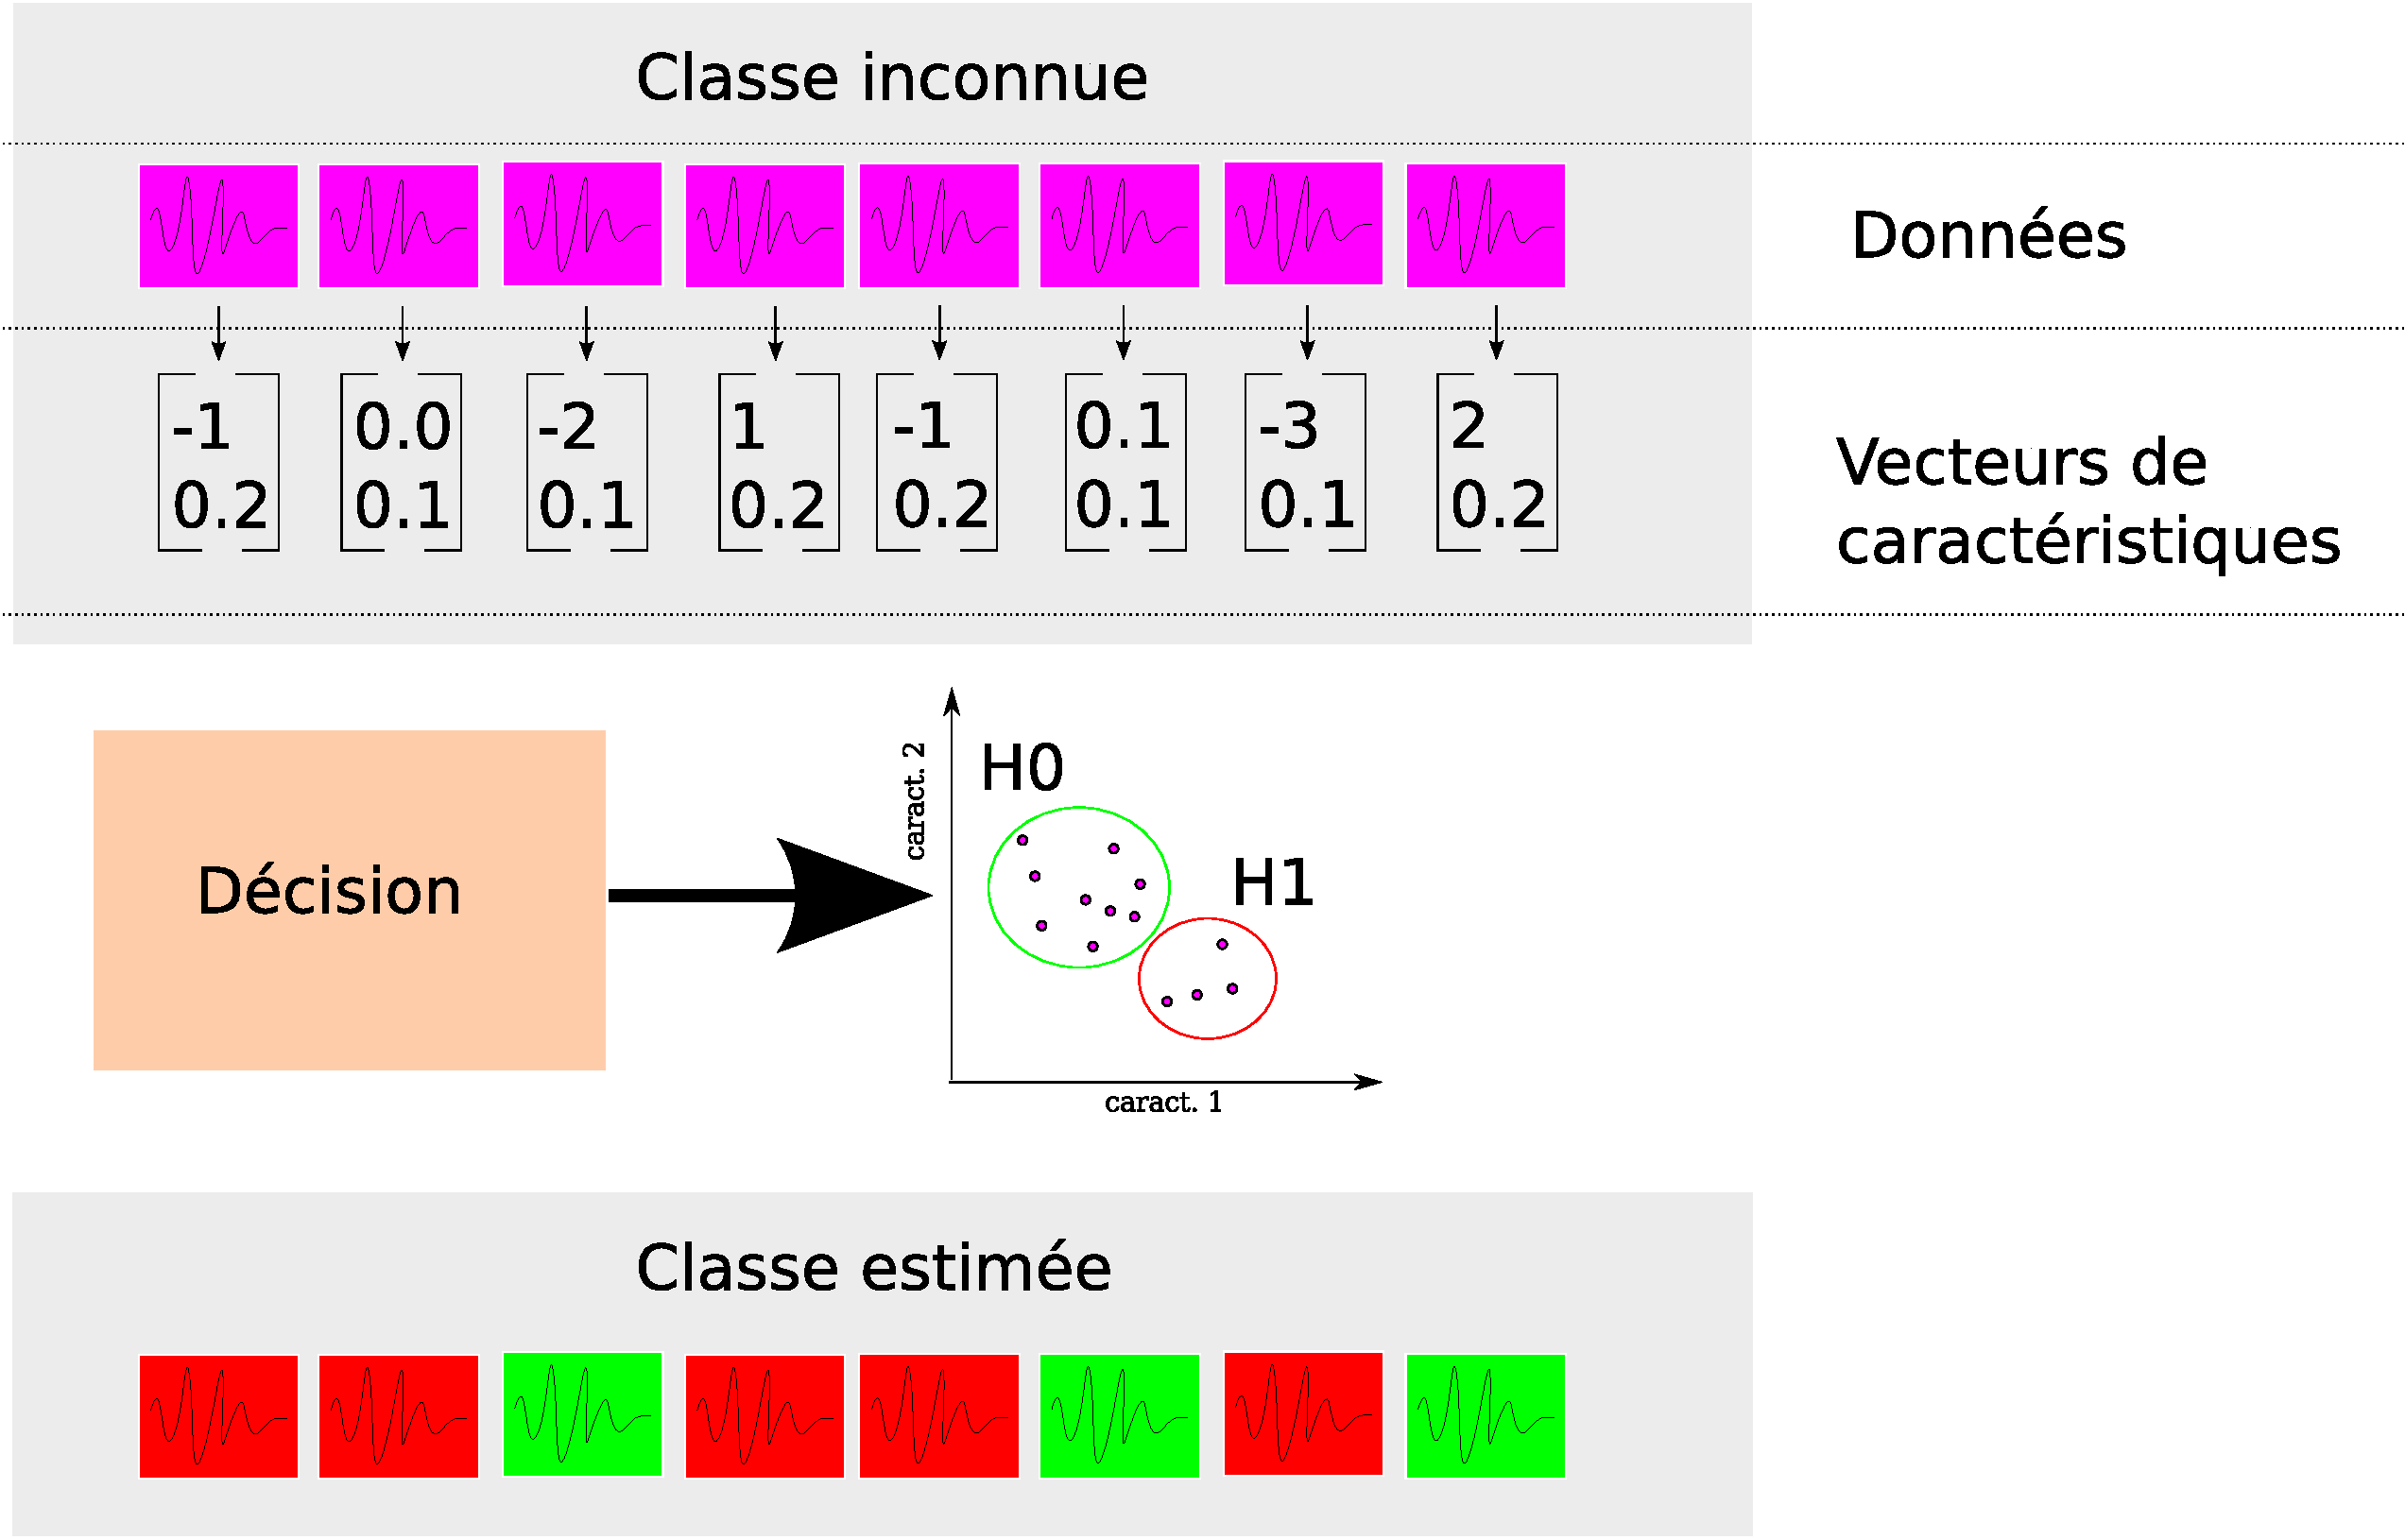
\includegraphics[width=15cm]{images/fonctionnementClassifNonSup}
	\end{center}
	\caption[Fonctionnement d'un classifieur non supervisé]{Fonctionnement d'un classifieur non supervisé : Les données brutes sont envoyées au classifieur qui va les regrouper en classes en fonction de leur répartition dans l'espace des caractéristiques.}
	\label{fig:fonctionnementClassifNonSup}
\end{figure}


		\subsection{Méthodes supervisées}

La classification supervisée vise à étiqueter des observations à partir de connaissances acquises \textit{a priori}.

Les classifieurs supervisés nécessitent une connaissance \textit{a priori} des classes. On entraîne le classifieur en lui fournissant des \emph{exemples} de cas avec l'étiquette associée. A partir de cette base de données d'entraînement, le classifieur va générer un \emph{modèle} prédictif permettant de classer de futurs exemples non encore connus, comme présenté dans la figure~\ref{fig:fonctClassif}.

\begin{figure}[h]
	\begin{center}
	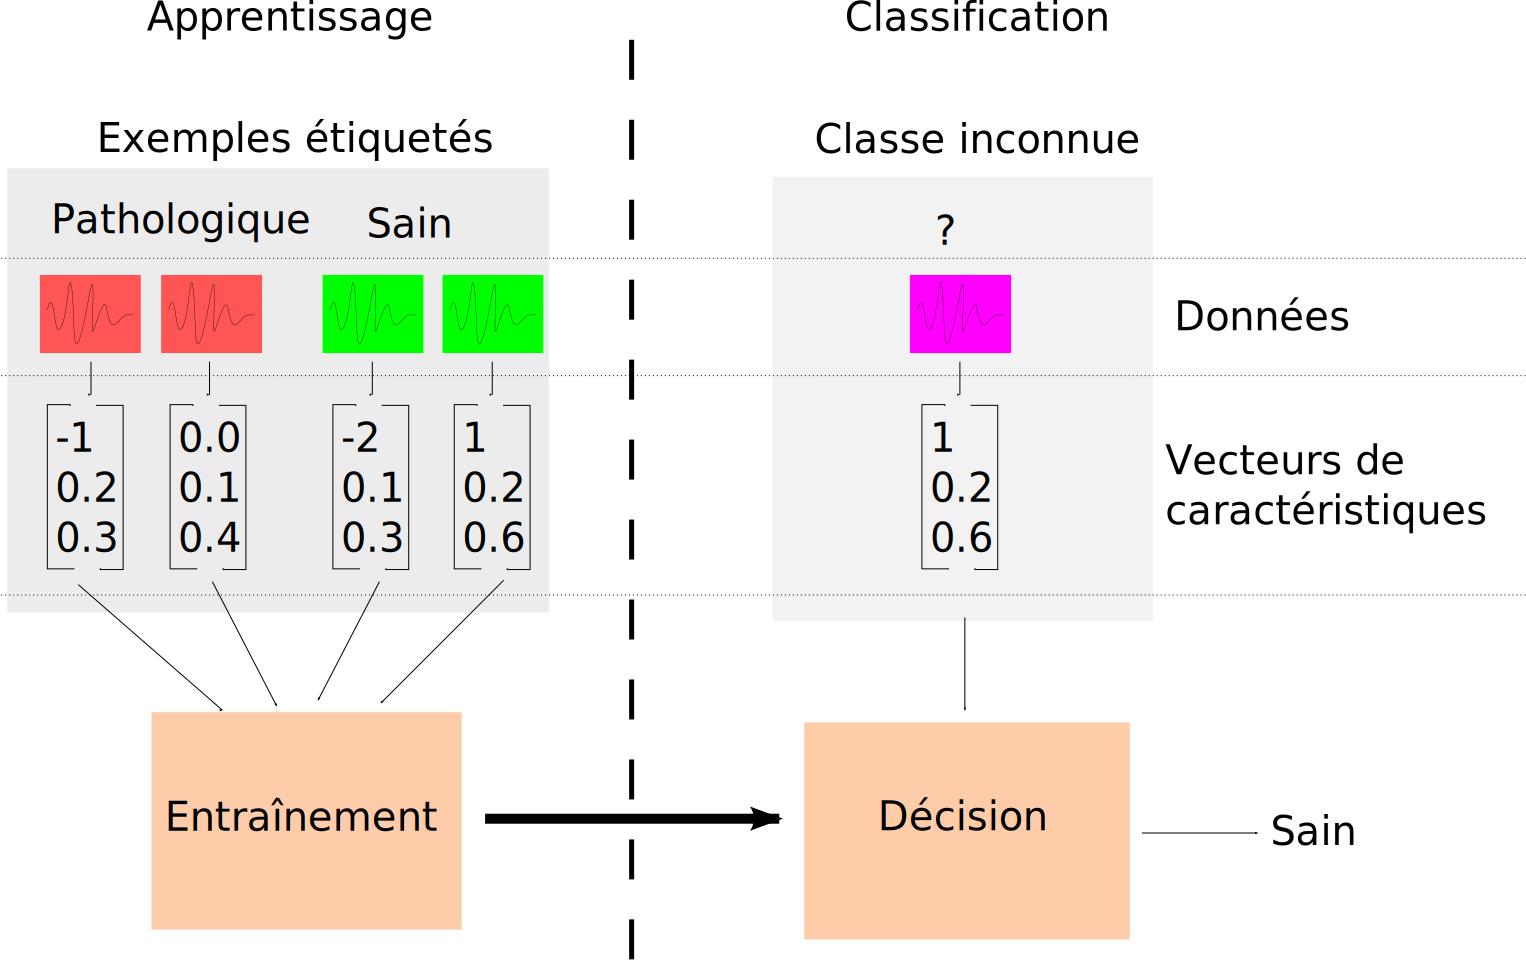
\includegraphics[width=15cm]{images/fonctionnementClassif}
	\end{center}
	\caption[Fonctionnement d'un classifieur supervisé]{Fonctionnement d'un classifieur supervisé : Les données d'apprentissage servent à entraîner le classifieur pour générer un modèle. Ce modèle permettra de rattacher des observations aux classes apprises.}
	\label{fig:fonctClassif}
\end{figure}


	\section{Machines à vecteur de support (SVM)}

\label{lab:SVM}
La ``Machine à Vecteur de Support'', aussi appelée ``Séparateur à Vaste Marge'', ou ``Support Vector Machine'' en Anglais, est un classifieur qui comme son nom l'indique vise à maximiser la marge~\cite{boser1992training}, qui est la distance minimale entre les points des données et la surface séparatrice (voir figure~\ref{fig:SVM}).

\begin{figure}[h]
	\begin{center}
	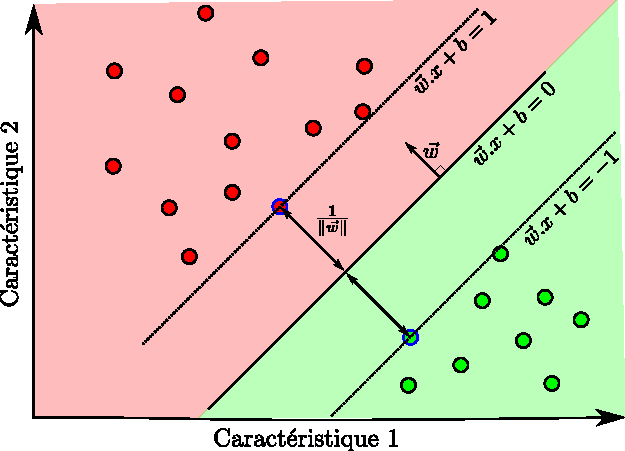
\includegraphics[width=11cm]{images/SVM}
	\end{center}
	\caption[Machine à Vecteur de Support]{Machine à Vecteur de Support : les points vecteur de support (entourés de bleu) sont les seuls utilisés pour calculer la surface de séparation d'équation $w . x + b = 0$. Le vecteur $w$ est normal à la surface de séparation et permet de calculer la marge $\frac{1}{\Vert w \Vert}$.}
	\label{fig:SVM}
\end{figure}


Les SVM sont des classifieurs supervisés qui cherchent à maximiser la séparation entre chaque classe. L'idée sous-jacente aux SVM est de trouver l'hyperplan optimal de séparation, et non pas n'importe quel hyperplan qui permettrait de séparer correctement les données d'apprentissage (figure~\ref{fig:multiPlansSeparationSVM}). 


\begin{figure}[h]
	\label{fig:multiPlansSeparationSVM}
	\begin{center}
	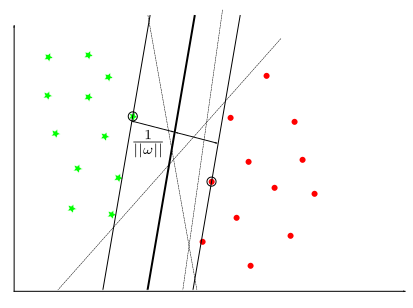
\includegraphics[width=11cm]{images/multiPlansSeparationSVM}
	\end{center}
	\caption[Illustration du principe d'optimisation de la marge sur le SVM]{Illustration du principe d'optimisation de la marge sur un cas à deux classes et deux caractéristiques : Il existe une infinité d'hyperplans qui séparent correctement les classes ``étoile vertes'' et ``ronds rouges'', représentés par les traits fins en pointillé. Cependant, il existe seulement une seule solution qui maximise la marge. Cette solution est représentée en trait plein, avec la marge $\frac{1}{||w||}$. Les points entourés en noir sont les points support utilisés pour contraindre l'hyperplan. }
\end{figure}


La définition de la marge et de l'hyperplan se fait à partir des vecteurs de support. Ils correspondent aux cas extrêmes des deux classes qui pourraient éventuellement poser des problèmes de classification.


Soit $\{(x_i, y_i) | x_i \in \mathbb{R}^p , y_i \in \{ -1, 1 \} \}$ un ensemble de points étiquetés correspondant à la base d'apprentissage. $x_i$ correspond au vecteur caractéristique, tandis que $y_i$ correspond à la classe du point.

Tout hyperplan dans l'espace des caractéristiques $\mathbb{R}^p$ peut être écrit $w . x - b = 0$, avec $w$ la normale à l'hyperplan et $\frac{b}{ ||w|| }$ le décalage de l'hyperplan par rapport à l'origine. 

La contrainte principale sur $w$ et $b$ est de classer correctement les données. Pour cela, les points vecteur de support devront respecter la contrainte $y_i ( w . x_i - b ) >= 1$. Par construction, les vecteurs de support correspondent aux points où l'égalité stricte est observée : $y_i ( w . x_i - b ) = 1$, comme indiqué sur la figure~\ref{fig:SVM}.

La seconde contrainte est la maximisation de la marge, qui correspond à  $\frac{2}{||w||}$, ce qui revient à minimiser $||w||$ comme indiqué sur la figure~\ref{fig:multiPlansSeparationSVM}.

La solution de ce problème d'optimisation est apportée par l'algorithme des multiplicateurs de Lagrange. 

Cependant, il peut arriver que les classes ne soient pas séparables. Ce problème est résolu par l'autorisation d'une erreur~\cite{cortes1995support} $\xi_i$  que l'on cherchera à minimiser : $( w . x_i - b ) >= 1 - \xi_i $. Cela engendre l'ajout d'un paramètre noté $C$, qui sera utilisé dans le lagrangien pour pénaliser plus ou moins les erreurs.

Dans le cas où l'hyperplan de séparation ne pourrait pas être défini par une équation linéaire, des fonctions à noyaux sont utilisées pour projeter les points dans un espace de plus grande dimension où le problème devient linéaire (voir figure~\ref{fig:kernelTrick}). Cependant, le passage des points dans l'espace de dimensions supérieure n'est jamais réalisé explicitement, car en pratique, le changement de dimension est utilisé uniquement lors de la comparaison entre deux points. On utilise donc des fonctions de comparaison modifiées, appelées noyaux, qui réalisent cette transformation de manière implicite. Le noyau le plus couramment utilisé est le RBF (fonctions à base radiale) qui utilise un espace d'arrivée de dimensions infinies, ce qui est rendu possible par le fait que l'on ne réalise par la transformation directement, mais qu'elle est réalisée implicitement lors de la comparaison des points $x_i$ et $x_j$ à l'aide de l'équation suivante :

\begin{equation}
k(x_i,x_j)=e^{-\gamma||x_i-x_j||^2}  
\end{equation}

\begin{figure}[h]
	\begin{center}
	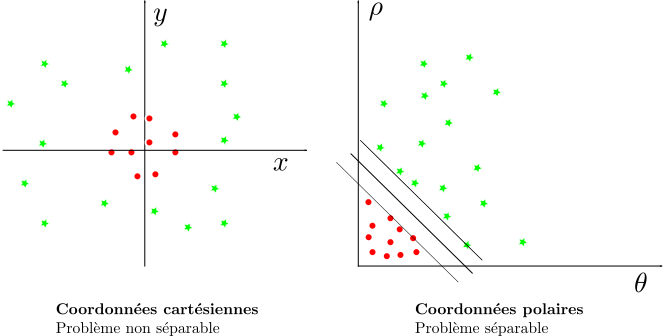
\includegraphics[width=15cm]{images/kernelTrick}
	\end{center}
	\caption[Changement de base pour les SVM]{Illustration du principe du changement de base : Des données non séparables dans le repère original peuvent devenir séparables en utilisant les noyaux. Dans ce cas, le passage des coordonnées cartésiennes aux coordonnées polaires permet de rendre le problème original linéairement séparable.}
	\label{fig:kernelTrick}
\end{figure}


Grâce à la maximisation de la marge, les SVM sont performants dans le cas où l'on ne dispose que de faibles quantités de données. D'autres algorithmes tels que les forêts aléatoires parviennent à obtenir des performances similaires~\cite{statnikov2008comprehensive}.

\subsection{Autres classifieurs supervisés}

De nombreux classifieurs supervisés ont été développés :

\label{lab:LDA}
Le classifieur LDA~\cite{fisher1936use} approxime les deux classes en supposant qu'elles ont une distribution gaussienne de covariance égale. Seule la moyenne de chaque distribution varie, et tout nouveau point est classé en fonction de sa distance à l'une ou l'autre des classes. Bien qu'il soit très rapide, ce classifieur ne fonctionne que dans le cas linéaire. L'approximation gaussienne donne des résultats suffisamment bons dans de nombreux cas, ce qui explique son utilisation pour la détection des lésions en mammographie~\cite{baydush2007incorporation} ou en oncologie TDM~\cite{gurcan2002lung} par exemple.


Les réseaux de neurones~\cite{haykin1999neural} sont des classifieurs non linéaire qui se basent sur un fonctionnement simplifié des neurones du cerveau humain. ils sont constitués de neurones artificiels qui miment les réactions des neurones biologiques. Un neurone applique une fonction à la combinaison linéaire de ses stimuli d'entrée. Chaque élément du vecteur de caractéristique est entré dans un neurone, qui ira stimuler un ou plusieurs autres neurones. L'information se propage jusqu'à un neurone terminal qui donnera le résultat. Les réseaux de neurones sont très performants, mais souffrent de difficultés de mise en place à cause de leur grand nombre de paramètres et de temps d'apprentissage très importants.

Une forêt de décision est un classifieur relativement récent basé sur plusieurs arbres de décisions initialisés différemment~\cite{ho1998random}. Le résultat de ce classifieur est le mode des résultats de tous les arbres. La combinaison de plusieurs arbres différents permet d'améliorer la stabilité du classifieur, qui est un gros désavantage des arbres de décision pris indépendamment. Ce classifieur est très rapide et très performant.




\part{Construction d'une base d'images TEP simulées respirante}
	\chapter{Simulations}

Simuler des images réalistes est un enjeu important en imagerie médicale. Le fait d'avoir accès à la vérité terrain, contrairement à la routine clinique, permet de valider des hypothèses de manière beaucoup plus fine. De plus, avec l'augmentation des performances de ordinateurs et l'accès à des centres de calculs, il devient possible de créer des bases de données de patients de plus en plus importantes et réalistes.

Nous allons tout d'abord présenter les différents types d'algorithme de simulations disponibles. Ensuite, nous ferons un état de l'art des simulateurs développés par la communauté. Enfin, nous décrirons le simulateur retenu ainsi que les contributions réalisées pour générer la base de données.

	\section{principe des simulations}

		\subsection{Simulations analytiques}

Les simulateurs analytiques utilisent des approximations fortes pour résoudre les problèmes de manière analytique. Il ne simulent pas de manière réaliste le déplacement des particules (positon, photon) comme les simulateurs Monte-Carlo.

Dans le cas de l'imagerie TEP, la simulation analytique revient à réaliser des projections du volume TEP dans l'espace du sinogramme. Ce sinogramme est ensuite bruité et modifié pour prendre en compte les effets des coïncidences aléatoires et des photons diffusés. L'efficacité des détecteurs est aussi prise en compte, tout comme les effets de l'atténuation. 

La reconstruction est ensuite réalisée de manière classique à l'aide des algorithmes de reconstruction TEP.


Cependant, bien que ce type de simulateur soit extrêmement rapide, les images générées ne parviennent pas à reproduire de manière parfaite les différents phénomènes physiques à l'origine du bruit.




		\subsection{Simulation Monte-Carlo}

Les simulations Monte-Carlo\footnote{Le nom de Monte-Carlo fait allusion aux jeux de hasard pratiqués dans la ville du même nom.} (MC) ont une approche probabiliste en modélisant la trajectoire de chaque photon indépendamment. .

Dans le cadre de l'imagerie TEP, le modèle probabiliste est appliqué à l'émission, puis au parcours du positon, à son annihilation, ainsi que les interactions et la probabilité de détection des photons dans les détecteurs.

La génération et le suivi de chaque photon ainsi que de chaque désintégration prennent un temps extrêmement important, amplifié par le fait que deux désintégrations successives dans des organes différents peuvent amener à une coïncidence fortuite. Il faut aussi prendre en compte les limitations de l'électronique (incapacité à séparer des évènements trop proches en temps comme en énergie, saturation des capteurs, \dots) ce qui amène à des temps de simulation prohibitifs de l'ordre de plusieurs mois, même sur des centres de calculs. Le grand Challenge TERA 10 crée en 2006 a mobilisé un supercalculateur comprenant 7000 processeurs pendant 3h pour simuler une image corps entier à l'aide du simulateur GATE, avant la mise en place des procédures d'accélérations. Cela revient à plus 10 jours de calculs ininterrompus pour une soumission sur centre de calculs avec 100 processeurs disponibles en permanence.

	\subsection{Simulation Monte-Carlo accélérées}

Les simulateurs Monte-Carlo accélérés utilisent des heuristiques pour augmenter la vitesse des calculs, notamment en réalisant des calculs préliminaires afin de simplifier les simulations futures. 

La séparation des simulations entre les coïncidences directes et diffusées, à l’aide des statistiques créées précédemment, permet encore d’accélérer les calculs. Le projet ANR fGATE a permis une amélioration des temps de calcul d'un facteur 20 par rapport à ceux présentés ci-dessus.

	\section{\'Etat de l'art des simulateurs TEP}

De nombreux simulateurs ont été développés par la communauté. Ils sont souvent développés à partir d'une librairie dédiée aux calculs de trajectoires de particules, comme GATE~\cite{jan2004gate}, qui se base sur le jeu d'outils de simulation d'interactions particule/matière Geant4~\cite{allison2006geant4}, le simulateur Penelo-PET\cite{espana2009penelopet} basé sur la librairie de simulation  PENELOPE~\cite{salvat2006penelope}, ou encore EGS-PET. L’université de Washington développe le simulateur Monte-Carlo simSET ainsi que le simulateur analytique ASIM. 

De très nombreux simulateurs ont été développés en interne par de petites équipes pour les besoins des laboratoires, mais ils s'orientent actuellement  vers GATE, qui bénéficie d'un développement rapide et d'une grande communauté.

Une étude décrit l'ensemble des codes disponibles en 2002~\cite{buvat2002monte}, et a été mise à jour en 2006~\cite{buvat2006monte} pour prendre en compte les avancées techniques réalisées.

Nous avons utilisé PET-SORTEO, car il a été développé pour augmenter la vitesse de simulations et profiter de la parallélisation offerte par les centres de calculs. De plus, nous avons réalisé à CREATIS la première version de la base de données OncoPET\_BD~\cite{tomei2010oncopet_db} sur ce simulateur, ce qui permet de capitaliser sur l’expérience déjà acquise. 

	\section{Processus de simulation avec SORTEO}
\label{lab:simuSORTEO}
Pour reproduire les données fournies par les systèmes cliniques TEP, les simulateurs Monte-Carlo simulent les désintégrations une par une et suivent les sous-produits dans les tissus jusqu'aux détecteurs. Étant donné qu'un examen TEP génère plusieurs millions de désintégrations, les temps de simulations deviennent très rapidement prohibitifs. PET-SORTEO dispose de plusieurs heuristiques qui permettent d'accélérer les simulations, notamment en séparant les simulations des différents types de coïncidences en fonction de statistiques estimées au début de la simulation. Cependant il faut tout de même encore plusieurs dizaines d'heures pour simuler une image correspondant à une acquisition clinique TEP corps entier au $^{18}$FDG.

a) Le logiciel prend en entrée deux cartes de labels voxelisées correspondant respectivement au type de traceur et à sa concentration (en $Bq/cm^3$), ainsi qu'à l'atténuation pour chaque voxel. A chaque label (nombre entier définissant une région) correspond un organe, qui peut être différent pour les deux cartes. Le type de scanner doit être précisé, ainsi que les paramètres d'acquisition (2D ou 3D), et le format de sortie (mode séquence ou sinogramme).

Toutes ces informations sont stockées dans un fichier texte, appellé fichier de protocole. Les cartes d'émission et d'atténuation voxeliques doivent être fournis au format ECAT (développé par Siemens).

b) Ensuite, la première partie de la simulation est utilisée pour déterminer un ensemble de probabilités permettant d'accélérer les calculs futurs. Pour cela, SORTEO réalise des simulations Monte-Carlo complètes pour chaque label avec un faible nombre de photons. Cela permet de calculer plusieurs grandeurs telle que la probabilité de détection des photons pour chaque couple (label, détecteur) en prenant en compte les phénomènes physiques, ou encore la probabilité de détection en coïncidence des deux photons émis lors d'une désintégration pour chaque label.

c) La seconde partie de la simulation correspond à la réalisation de l'examen proprement dit. C'est à cette étape que sont simulées les coïncidences vraies, qu'elles soient diffusées ou non. Chaque coïncidence de chaque label est simulée une par une, et le trajet de chaque photon est calculé séparément. Si un des photons est absorbé ou si son énergie n'est pas dans la fenêtre énergétique déterminée par les paramètres d'acquision, alors la paire de photons est considérée comme perdue. Le programme passe à la désintégration suivante. \`A cette étape, le programme prend en compte les temps morts (limitation de l'électronique qui ne peut pas prendre en compte un trop grand nombre de photons en même temps), qui dépend de l'activité. Il est intéressant de noter que grâce aux statistiques estimées à la première étape, la trajectoire de certains photons n'est pas calculée car le simulateur considère qu'ils font partie des ``pertes``. C'est ce qui permet de réaliser les calculs très rapidement par rapport aux simulations Monte-Carlo classiques.

d) La dernière étape consiste à simuler les coïncidences aléatoires, qui sont ajoutées aux données précédentes. Ces dernières sont calculées à l'aide d'un modèle utilisant les paramètres mesurés à l'étape b), notamment le taux de photons simples arrivant sur chaque détecteur.


Le modèle utilisé par SORTEO est un compromis intéressant entre le réalisme apporté par les méthodes de Monte-Carlo et les performances apportées par les techniques de pré-calculs de statistiques ainsi que de séparation du calcul des coïncidences directes et fortuites. L'auteur de PET-SORTEO annonce que toutes les sources majeures de bruit et de biais sont prises en compte.

Le simulateur PET-SORTEO a été validé pour le simulateur Ecat Exact HR+~\cite{reilhac2004pet} ainsi que pour la plateforme PET Philips Allegro, qui est à la base du scanner TEP/TDM Gemini~\cite{lemaitre2008}. 


	\section{Contribution à PET-SORTEO}

Au cours de cette thèse, nous avons effectué plusieurs contributions au code de PET-SORTEO, notamment au niveau de la partie découpage des tâches pour l'exécution en centre de calcul, et au niveau de l'adaptation du programme aux données séquences.

\subsection{Adaptation pour l'exécution sur centre de calcul}

Le code original de SORTEO était adapté à une exécution sur des centres de calculs de petite taille, où la communication entre les processus n’est pas limitée. Cependant, étant donné les volumes de calculs représentés par nos simulations, nous avons fait appel au centre de calcul de l'in2p3 (Institut National de Physique Nucléaire et de Physique des Particules).

Ce centre de calcul regroupe plus de 1300 machines totalisant plus de 17000 cœurs, ainsi que 13 PetaOctets de stockage sur disques en 2011. Les technologies mises en places par les administrateur du centre de calcul sont spécialisées pour gérer cette quantité de données, ce qui représente des contraintes particulières quand aux techniques employées par les logiciels.

Par exemple, les différents processus du simulateur PET-SORTEO dialoguaient à travers des fichiers partagés. Cela engendrait des problèmes de saturation de la bande passante entre les nœuds. J'ai donc réalisé des modifications en profondeur du code pour séparer le simulateur en plusieurs entités, chacune réalisant une seule partie du travail :

    \begin{enumerate}
        \item Estimation des paramètres nécessaires à la simulation accélérée par simulation Monte-Carlo pur (lancé pour chaque processus).
        \item Combinaison des résultats Monte-Carlo.
        \item Simulation simplifiée des désintégrations (lancé pour chaque processus).
        \item Combinaison des désintégrations détectées pour chaque processus dans un seul fichier de données.
    \end{enumerate}

Ensuite, un ensemble de scripts a été réalisé pour automatiser les opérations de combinaison des résultats et de calcul des statistiques, puis pour relancer les simulations des coïncidences vraies et fortuites. Une dernière étape consiste à réassembler les détections pour générer les données séquence.

\subsection{Sortie en mode Séquence}

Bien que le code original permettait de spécifier un format de sortie, en pratique seul le format sinogramme était pris en compte. 

En effet, le code original ne permettait pas la sauvegarde de l'information temporelle de chaque évènement détecté. Or cette information est nécessaire aux méthodes de correction du mouvement respiratoire. 

Nous avons donc adapté PET-SORTEO au format séquence. Nous avons repris le format LMF développé lors de la collaboration CrystalClear pour générer les données, car ce format de données est simple à utiliser. Il se compose d'un fichier texte comprenant les informations sur l'acquisition ainsi que d'un fichier binaire contenant les évènements organisés de manière séquentiel.

 L'adaptation de SORTEO a nécessité entre autres ces adaptations :

\begin{itemize}
\item Intégrer la spécification du format de sortie dans le code.
\item Intégrer dans le code de PET-SORTEO des enregistreur d'évènements pour chaque désintégration détectée, car le code original se contentait de modifier un sinogramme. Cela a nécessité une modification en profondeur du code original.
\item Adapter la géométrie du modèle simulé pour correspondre aux conventions du LMF.
\item Ajouter une information temporelle non présente originellement à chaque évènement.
\item Réaliser le code permettant l'assemblage et le tri de toutes les émissions, qui sont réalisées séparément pour chaque organe.
\end{itemize}


%%%%%%%%%%%%%%% PARTIE RECONSTRUCTION ENVOYEE DANS METHODES


	\chapter{Base de données : OncoPET_Respi}
	\label{lab:bdd}

\section{Présentation}

Pour répondre à notre problématique de détection des lésions sur les images TEP respirantes, nous avons choisi d’utiliser une base de données d’images simulées. En effet, notre problématique repose sur une connaissance très précise de la position des lésions pour l’évaluation des performances, ainsi que sur l’acquisition de données en mode séquences. Ces deux objectifs sont relativement difficiles à atteindre à partir d’images cliniques, notamment parceque l'acquisitio nen modé séquence ne fait pas partie de la routine clinique en oncologie.

	\subsection{Avantages des bases de données simulées}

Le principal avantage des bases de données est le contrôle qu'elles permettent d'exercer sur les modèles. Il est possible de spécifier les conditions des acquisitions de manière très précise, et garantissent une homogénéité qu'il est difficile d'atteindre en utilisant des données patient.

Dans le cadre de nos travaux sur la détection, la présence de la vérité terrain est particulièrement appréciable, car elle permet de savoir avec une certitude impossible à atteindre en clinique la position, le contraste et le nombre des lésions. En effet, dans le cas de lésions de petit diamètre et de petit contraste, le diagnostic ne peut être donné avec une précision totale par le praticien. 

De plus, les simulations permettent d’obtenir des images avec des paramètres qui ne sont pas forcément disponibles en routine clinique. Dans notre cas, la génération des images en mode séquence est indispensable, et très peu d’examens sont réalisés de cette façon, notamment à cause de l’espace disque nécessaire et des temps de reconstruction.

	\section{Modèles}

Nous avons utilisé une base de données d’images TDM fournie par le Centre Hospitalier Lyon-Sud (CHLS) pour créer 15 modèles. Cette variabilité des patients va permettre de limiter le sur-apprentissage des outils de détection. Le fantôme paramétrique XCAT~\cite{segars2009mcatoverview} développé par Paul Segars a été adapté  sur chacune des images TDM à l’aide d’un logiciel fourni avec le modèle, présenté dans la figure~\ref{fig:fitXCAT}. Ce modèle est basé sur des courbes paramétriques NURB (Non-Uniform Rational B-Splines) que l'on peut ajuster manuellement sur les organes d'interêt du patient en déplacant les points de contrôle. Le recalage n’est pas parfait, du fait des limitations du logiciel, mais permet d’obtenir une variabilité suffisante pour notre étude. Deux images TDM associés aux fantômes adaptés sont présentés dans la figure~\ref{fig:adaptXCAT}.

\begin{figure}
 \centering
 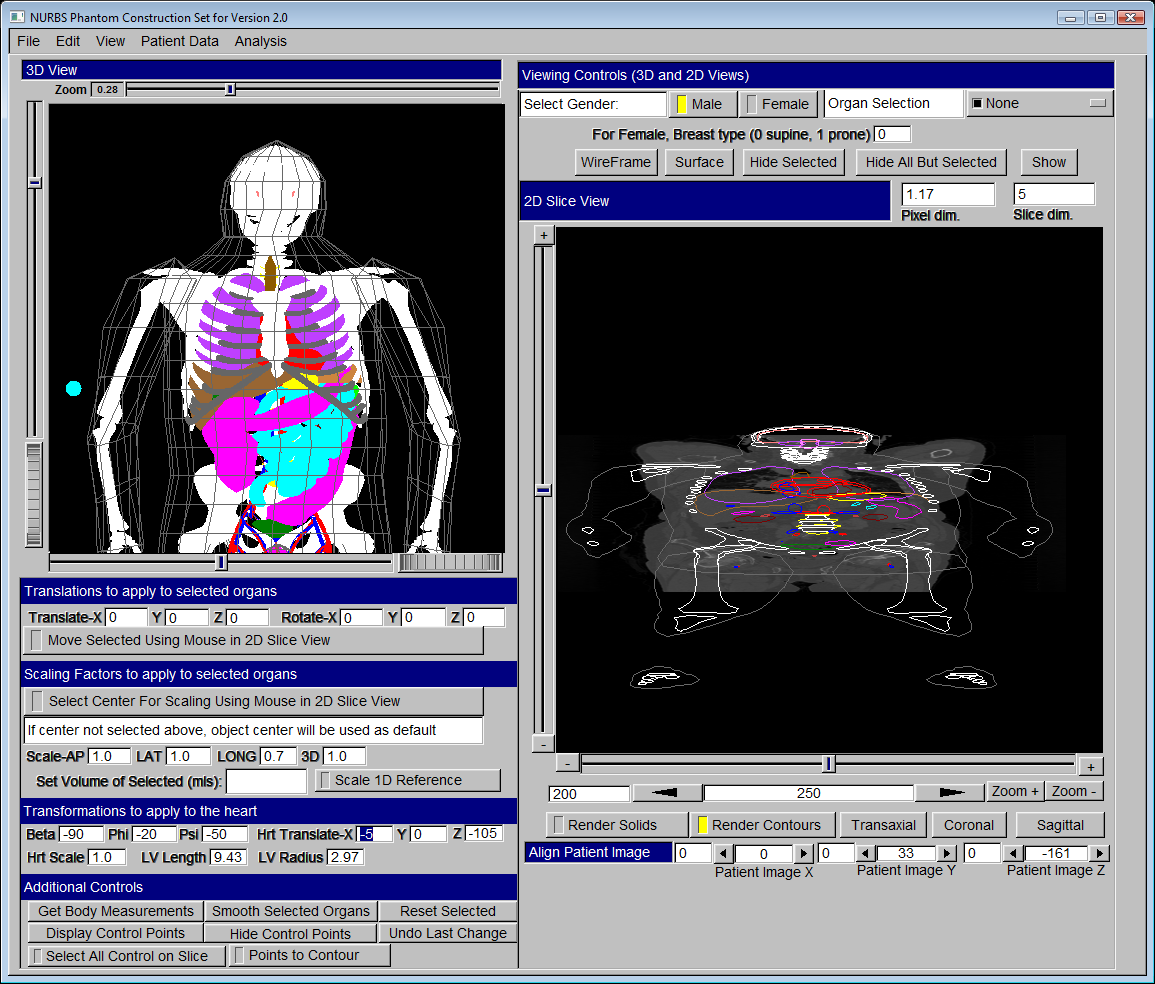
\includegraphics[width=10cm]{images/FIT_XCAT}
 \caption[Adaptation du modèle XCAT sur une image TDM de patient]{Adaptation du modèle XCAT sur une image TDM de patient : le modèle est fortement déformé par la différence entre l'épaisseur des coupes et la résolution du plan. Chaque organe est représenté par une surface paramétrique qu’il est possible d’adapter sur un modèle de patient.}
 \label{fig:fitXCAT}
\end{figure}

Nous avons choisi le XCAT car il intégre directement un modèle de mouvement respiratoire, et il est conçu pour pouvoir être déformé et créer différents patients.

\begin{figure}
 \centering
 \begin{tabular}{c c}
 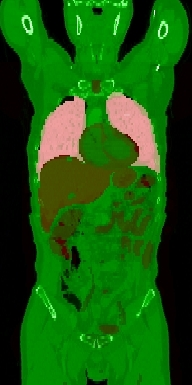
\includegraphics[width=6cm]{images/adapt_bru_jea} &
 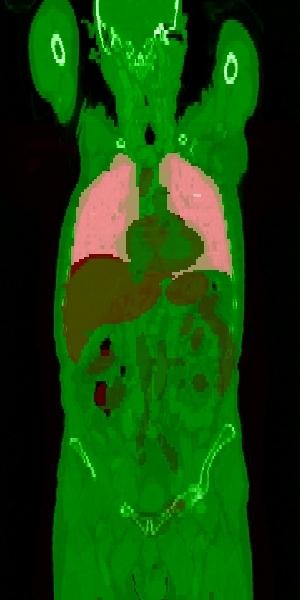
\includegraphics[width=6cm]{images/adapt_cha_chr}
 \end{tabular}
 \caption[Exemple d’adaptation d’images du modèle XCAT sur des images TDM]{ Exemple d’adaptation d’images du modèle XCAT sur des images TDM : deux modèles XCAT représentés en niveaux de rouge sont adaptés sur des images TDM représentées en vert}
 \label{fig:adaptXCAT}
\end{figure}


		\subsection{Respiration}


Pour prendre en compte la variabilité du cycle respiratoire (voir figure \ref{fig:variabCycle}), nous avons utilisé 4 cycles différents pour modéliser la respiration du patient. Un signal respiratoire complet a été acquis sur une durée de plusieurs minutes à l'aide d'un spiromètre (voir \ref{lab:spirometre}). Nous avons extrait 3 cycles semblables correspondants à la phase de respiration normale, ainsi qu'un cycle ``anormal'' pour prendre en compte une respiration irrégulière.

\begin{figure}
 \centering
 \begin{tabular}{c c}
 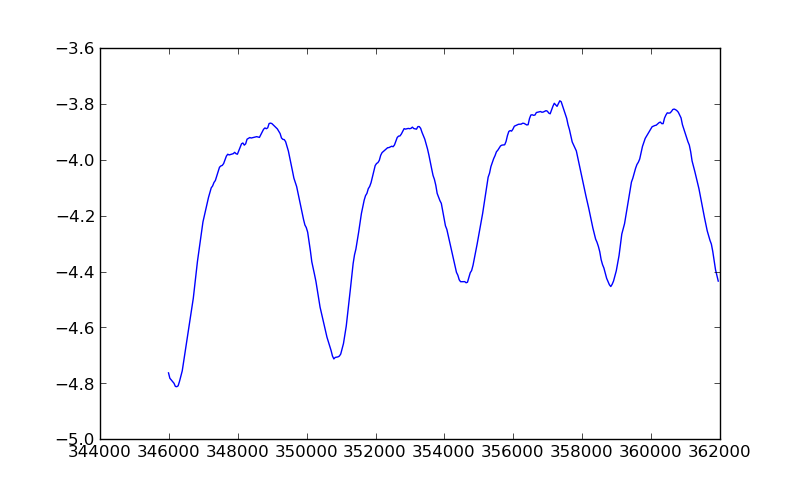
\includegraphics[width=8cm]{images/respiReguliere} &
 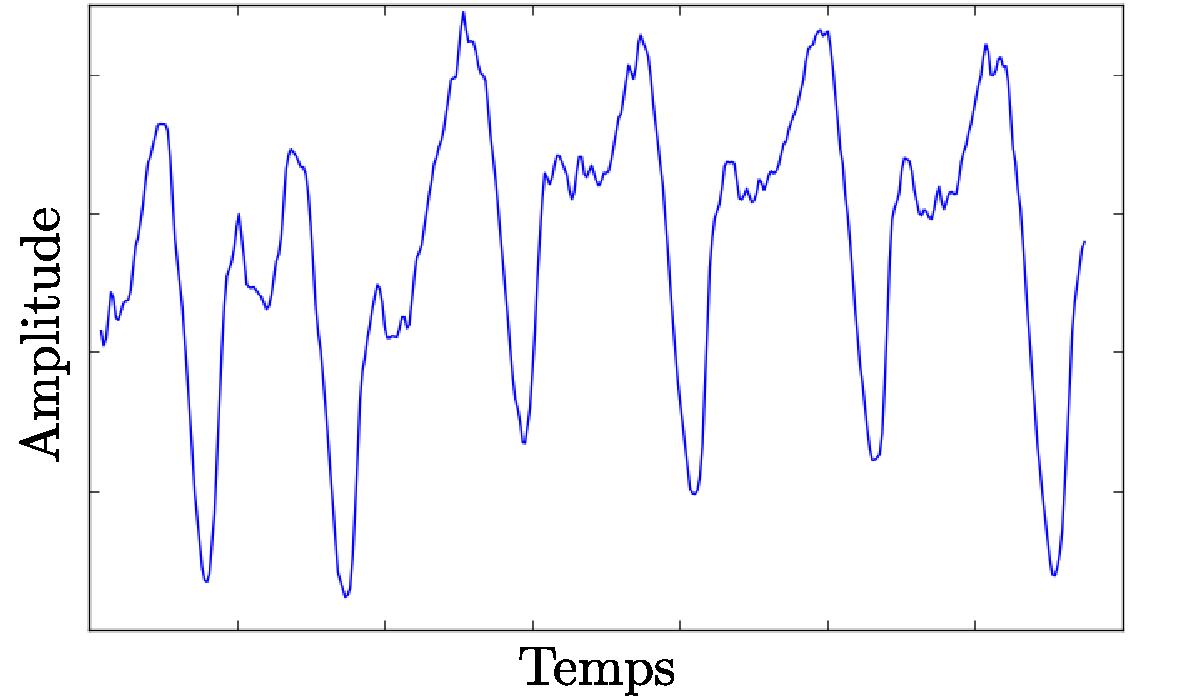
\includegraphics[width=8cm]{images/respiIrreguliere}
 \end{tabular}
 \caption[Exemple de courbes respiratoires régulière et irrégulière]{Deux exemples de courbes respiratoires prises par un spiromètre : celle de gauche montre une respiration régulière, tandis que celle de droite est irrégulière}
 \label{fig:variabCycle}
\end{figure}


La signal respiratoire obtenu est présentée dans la figure \ref{fig:cycleRespi}. Il est constitué de 4 cycles de 5.6 secondes qui se répètent 10 fois pour former un signal total de 224 secondes. 

Chacun de ces 4 cycles est discrétisé en 8 parties qui seront utilisées pour générer les modèles de la simulation. 


\begin{figure}
 \centering
 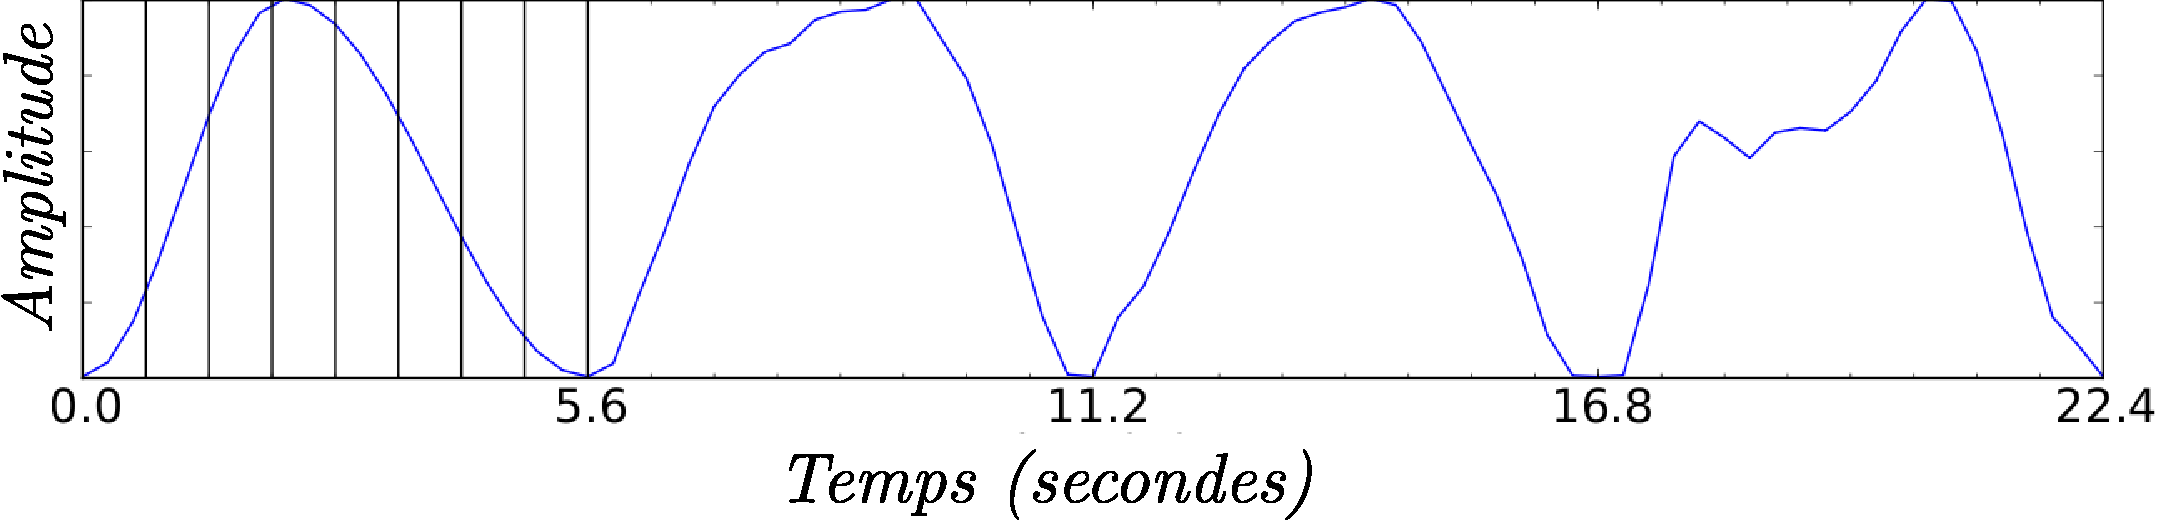
\includegraphics[width=12cm]{images/courbesRespi}

 \caption[signal respiratoire utilisé pour les modèles de la base de données]{Courbe respiratoire utilisée pour générer les modèles respirants. Les traits verticaux du premier cycle montrent les 8 instants sélectionnés pour discrétiser le mouvement respiratoire de ce cycle.}
 \label{fig:cycleRespi}
\end{figure}

	\section{Paramètres de simulation}

\subsection{Activités des organes}

Les activités des organes sont décrites dans la table \ref{tab:contrastePoumonFoieRecap}. Elles ont été estimées à partir d'une étude réalisée précédemment lors des travaux de thèse de Sandrine Tomeï~\cite{tomei2008development}, en mesurant l'activité dans des zones d'intérêt présentes dans les organes.

\begin{table}
\centering
 \begin{tabular}{|c|c|c|} 
\hline
Organe 		& Activité ($Bq/c^3$) \\
\hline
\hline
Foie		& 7740		       \\
\hline
Myocarde	& 11610		       \\
\hline
Os		& 3863		       \\
\hline
Poumon 		& 1338 		       \\
\hline
Prostate	& 2575		       \\
\hline
Rate		& 4939		       \\
\hline
Reins		& 8220		       \\
\hline
Sang		& 5340		       \\
\hline
Tissus mous 	& 2575 		       \\
\hline
Urètre		& 33815		       \\
\hline
Vésicule bilaire& 2575		       \\
\hline
Vessie		& 50973		       \\
\hline
 \end{tabular}

\caption[Activités des organes des patients de la base de données]{Activités définies pour les organes des patients virtuels}
\label{tab:activiteOrganes}
\end{table}

\subsection{Calibration des contrastes des lésions}

Notre but est de simuler des images avec un ensemble de tumeurs qui sont ni trop évidentes ni impossible à détecter. Nous avons donc cherché à obtenir une échelle de contrastes de tumeurs qui permette un taux de détection par un observateur humain de 10\%, 30\%, 50\%, 70\% et 90\%.

Pour réaliser cela, un ensemble d'images a été simulé sans mouvement respiratoire, avec différentes tailles de tumeurs. Ensuite, une étude ROC avec deux observateurs humains non médecin a été réalisée afin d'estimer la détectabilité de ces couples activité/taille de tumeurs (fig.\ref{fig:calibration}). 

Nous avons en premier lieu utilisé les contrastes présentés dans la base de données créée dans notre laboratoire et présentée dans~\cite{tomei2010oncopet_db}.

Nous avons simulé 5 réalisations d'un même modèle basé sur le XCAT avec plusieurs lésions implantées dans les poumons et le foie. Nous avons utilisé 4 \todo{nombre d'itérations à l'origine??}

Nous avons utilisé les contrastes de la base OncoPET_DB présentés dans la table~\ref{tab:contrastePoumonOrig} pour les lésions du poumon et dans la table~\ref{tab:contrasteFoieOrig} pour les lésions du foie.


\todo{combien de lésions, quelle taille/contraste}

\begin{table}
\centering
\begin{tabular}{|c||c|c|c|c|c|}
 \hline
Poumon	& 10\% & 30\% & 50\% & 70\% & 90\% \\
\hline
4mm	& 2    &  5   &  8   & 10   & 13   \\
\hline
12mm    & 2    &  5   &  8   & 10   & 13   \\
\hline
16mm    & 2    &  3.5 &  4.5 & 7.5  & 10   \\
\hline
\end{tabular}
\caption[Contraste de la base originale OncoPET\_DB des lésions du poumon pour létude de détectabilité]{Contraste de la base originale OncoPET\_DB des lésions du poumon, avec les pourcentages de détection associés}
\label{tab:contrastePoumonOrig}
\end{table}

\begin{table}
\centering
\begin{tabular}{|c||c|c|c|c|c|}
 \hline
Poumon	& 10\% & 30\% & 50\% & 70\% & 90\% \\
\hline
4mm	& 2.5    &  4   &  4.5   & 6   & 9   \\
\hline
12mm    & 2    &  3   &  4   & 4.5   & 7.5   \\
\hline
16mm    & 2    &  3   &  4   & 4.5   & 7.5   \\
\hline
\end{tabular}
\caption[Contraste de la base originale OncoPET\_DB des lésions du foie pour létude de détectabilité]{Contraste de la base originale OncoPET\_DB des lésions du foie, avec les pourcentages de détection associés}
\label{tab:contrasteFoieOrig}
\end{table}

On présente à chaque observateur les images les unes après les autres, qu'ils vont annoter en recherchant toutes les lésions et en leur attribuant une note à l'aide du logiciel Amide~\cite{loening2003amide}. Ils ne connaissent pas à l'avance la localisation des lésions, et doivent donner pour chaque lésion une note entre 1 et 5 correspondant au barème suivant :

\begin{enumerate}
\item Possible
\item Probable
\item Très probable
\item Pratiquement  certain
\item Certain
\end{enumerate}

Lors de cette étude, nous avons observé que les lésions de la base de données étaient beaucoup trop visibles, ce qui nous a amené à redéfinir les contrastes. 


Les figures~\ref{fig:calibration} et~\ref{fig:calibrationFoie}  représentent respectivement le taux de détection des lésions du foie et du poumon moyennée sur 2 observateurs en fonction du contraste.


\begin{figure}[h!]
\begin{center}
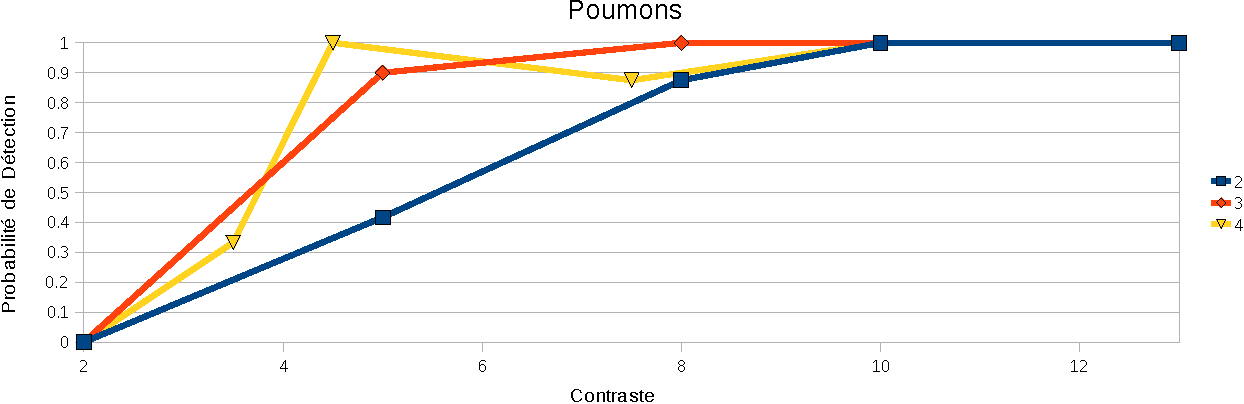
\includegraphics[width=15cm]{images/calibration_crop}
\end{center}
\caption{Détectabilité des tumeurs du poumon moyennée sur 2 observateurs en fonction du contraste et de la taille des tumeurs. Chaque courbe représente une taille de lésion différente} 
\label{fig:calibration}
\end{figure}

\begin{figure}[h!]
\begin{center}
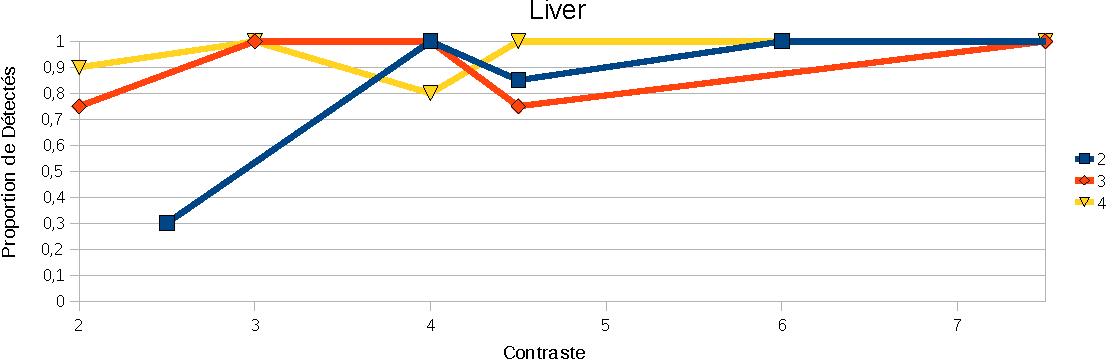
\includegraphics[width=15cm]{images/calibrationFoie_crop}
\end{center}
\caption[Détectabilité des tumeurs du foie en fonction du contraste et de la taille des tumeurs]{Détectabilité des tumeurs du foie moyennée sur 2 observateurs en fonction du contraste et de la taille des tumeurs. Chaque courbe représente une taille de lésion différente} 
\label{fig:calibrationFoie}
\end{figure}




\begin{table}
\centering
Poumon :\\
\begin{tabular}{|c|c|c|c|}
 \hline
 Détection voulue & 	8mm & 	12mm & 	16mm \\
\hline
90 \%		  & 100 \%  & 100 \% & 100 \% \\
\hline
70 \%		  & 100 \%  & 100 \% & 90 \%\\
\hline
50 \%		  & 90 \%  & 100 \% & 100 \%\\
\hline
30 \%		  & 44 \%  & 90 \% & 30 \%\\
\hline
10 \% 		  & 0 \%  & 0 \% & 0 \%\\
\hline
\end{tabular}

\vspace{0.5cm}

Foie :\\
\begin{tabular}{|c|c|c|c|}
 \hline
 Détection voulue & 	8mm & 	12mm & 	16mm \\
\hline
90 \%		  & 100 \%  & 100 \% & 100 \% \\
\hline
70 \%		  & 100 \%  & 75 \% & 100 \%\\
\hline
50 \%		  & 85 \%  & 100 \% & 75 \%\\
\hline
30 \%		  & 100 \%  & 100 \% & 100 \%\\
\hline
10 \% 		  & 30 \%  & 75 \% & 90 \%\\
\hline
\end{tabular}
\caption[Détectabilité estimée des lésions en fonction du contraste et de leur diamètre]{Détectabilité des lésions réalisée à l'aide d'une étude par des humains. La colonne de gauche indique la détectabilité calibrée pour OncoPET_BD des lésions.}
\label{fig:detectabiliteVue}
\end{table}

En pratique, les résultats sont résumés dans la table~\ref{fig:detectabiliteVue} et montrent une détectabilité largement supérieure à celle que nous avons estimé initialement à partir des résultats obtenus sur la première base de donnée. Les écarts peuvens s'expliquer par le fait que nous n'avons pas simulés le même scanner TEP (Caméra HR+ pour la base OncoPET\_BD, Philips Gemini pour la nouvelle base), et que les données ont été reconstruites avec un algorithme différent.

Après étude du tableau, il s'avère que les lésions de 16 mm sont trop visibles pour être intégrées dans l'étude. Nous avons fait des interpolations linéaires entre les statistiques obtenues pour définir les nouvelles activités, définies en \ref{tab:contrasteFoieFinal} pour le foie et le poumon.



\begin{table}

\centering

\begin{tabular}{|c||c|c||c|c|}
 \hline
	& 8mm Foie	& 12mm Foie	& 8mm Poumon	& 12mm Poumon	\\
\hline
10\%	& 1.8		& 1.3		& 3.0		& 2.5		\\
\hline
30\%	& 2.0		& 1.5		& 4.0		& 3.0		\\
\hline
50\%	& 2.5		& 1.8		& 5.0		& 3.5		\\
\hline
70\%	& 3.0		& 2.0		& 6.5		& 4.0		\\
\hline
90\%	& 3.5		& 2.3		& 8.0		& 5.0		\\
\hline
\end{tabular}
\caption[Contraste final lésions du foie et du poumon]{Contrastes appliqués aux lésions de la base de données en fonction du taux de détectabilité désiré.}
\label{tab:contrasteFoieFinal}
\end{table}



\section{Exemples de données simulées}

La base de données générée contient 15 patients, reconstruits avec une correction parfaite (image statique), sans correction, et avec deux méthodes de correction du mouvement respiratoire présentées en \ref{lab:corrPostRecon} et \ref{lab:CorrpendantRecon}. Un exemple d'images simulées est visible sur la figure~\ref{fig:exempleImageRecon}.

\begin{figure}
 \centering
 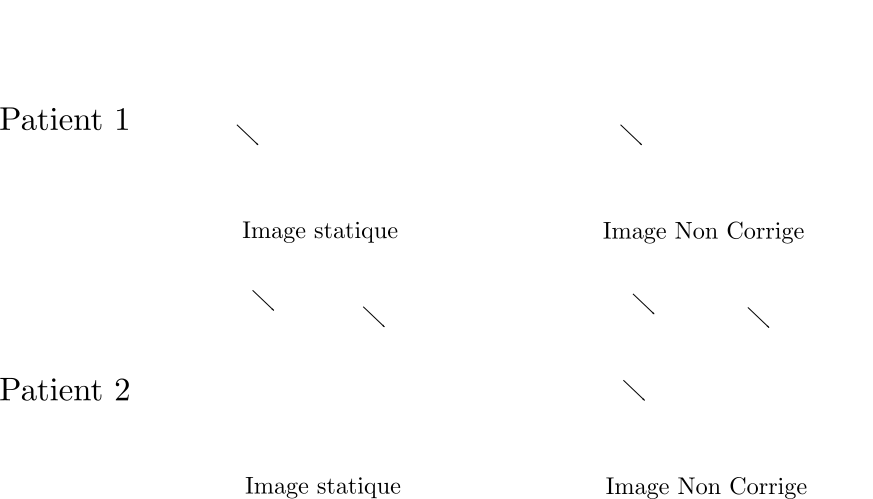
\includegraphics[width=10cm]{images/exempleImageRecon}
 \caption[Images reconstruites tirées de la base de donnée]{Images reconstruites tirées de la base de données. La flèche représente une lésion du poumon de diamètre 8mm avec une activité de niveau 5.}
 \label{fig:exempleImageRecon}
\end{figure}

\todo{plus d'images dans cette figure. Mais sans TE-IM et TE-MS}


	\section{Données clef} % temps de calculs etc....

\subsection{Modèles}

Nous avons crée 15 modèles, qui ont été adaptés depuis autant d'images TDM fournies par le centre hospitalier Lyon-SUD. Pour cela nous avons utilisé les outils fournis par Paul Segars~\cite{segars2001These}.


\subsection{Lésions}

Nous avons inséré 280 lésions dans les 15 modèles de patients que nous avons crée. 173 lésions sont présentes dans le Poumon, contre 103 dans le Foie. La différence de taille entre les organes explique la petite taille de la base de lésions du foie. 

Les lésions ont été placées manuellement dans tout le volume de l'organe, en préférant les parties à fort mouvement proche du diaphragme. 

Le tableau~\ref{tab:contrastePoumonFoieRecap} récapitule les contrastes, ainsi que les tailles des lésions implantées dans les organes.
 
\begin{table}
\centering
 \begin{tabular}{|c|c||c|c|c|c|c|} 
\hline
\multicolumn{2}{|c|}{Niveau de confiance}       & 1	  & 2	    & 3	     & 4	& 5	\\
\hline
\hline
Poumon	(173)	& 8 mm (90)	& 3 (19)  & 4 (18)  & 5 (18)  & 6.5 (18)	& 8 (17)\\
\cline{2-7}
		& 12 mm	(83)	& 2.5 (16)& 3 (16)  & 3.5 (18)& 4 (17)	& 5 (16)\\
\hline
Foie 	(107)	& 8 mm (54)		& 1.8 (11)& 2 (11)  & 2.5 (10)& 3 (11)	& 3.5 (11)\\
\cline{2-7}
		& 12 mm	(53)	& 1.3 (10)& 1.5 (10)& 1.8 (11)& 2 (11)  & 2.3 (11)\\
\hline 
 \end{tabular}

\caption[Tableau récapitulatif des lésions]{Tableau récapitulatif des contrastes des lésions présentes dans le foie et les poumon des modèles. Le nombre en parenthèse correspond au nombre de lésions}
\label{tab:contrastePoumonFoieRecap}


\end{table}


\subsection{Simulation et reconstruction}

Les images sont reconstruites avec des voxels de 4mm dans les trois dimensions. Les reconstructions sont réalisées à l'aide de l'algorithme OPL-EM avec 8 itérations et 5 sous-ensembles, sauf pour l'estimation de mouvement où seulement 3 itérations avec 5 sous-ensembles sont réalisées, avec une régularisation de 6mm à chaque itération. 

Le temps de simulation nécessaire pour générer une image statique est de 130h par processeur environ, et 110 heures pour générer une image dynamique.

Le volume de données généré est d'environ 6Go par patient sans prendre en compte les données intermédiaires générées lors de la simulation.




\part{\'Evaluation de la correction du mouvement respiratoire sur la détection des lésions pulmonaires et hépatiques}
	\chapter{Méthodes}

Nous avons utilisé la base de données présentée dans la partie~\ref{lab:bdd} pour évaluer les performances des techniques de correction du mouvement respiratoire présentées dans le chapitre \ref{lab:corrMvt}. 

Les techniques de correction du mouvement implémentées sont les suivantes :

\begin{enumerate}
 \item Correction pendant la reconstruction par modification de la matrice système (voir section \ref{lab:corrMatSyst}). Elle sera désignée par l'acronyme \emph{TE-MS} (Transformation \'Elastique de la Matrice Système)
 \item Correction post-reconstruction par recalage des images prises à différents instants du cycle (voir section \ref{lab:corrPostRecon}). Elle sera désignée par l'acronyme \emph{TE-IM} (Transformation \'Elastique des Images reconstruites) 
\end{enumerate}

Les images TEP corrigées à l'aide de ces deux méthodes sont comparées dans cette partie avec les images non corrigées et des images statiques (qui représentent une correction parfaite). Leur acronymes sont respectivement \emph{NoCorr} et \emph{Statique}.

L'objectif est d'évaluer les performances des techniques de correction du mouvement sur la détection des lésions de faible contraste et faible diamètre. Pour cela, les performances d'un système de détection automatique seront mesurées à l'aide des courbes F-ROC.

Ce chapitre va tout d'abord présenter la démarche réalisée pour sélectionner les paramètres de reconstruction des images, puis la méthode d'estimation du mouvement utilisée. 

La suite de ce chapitre présente les caractéristiques principales du système d'aide à la détection (CAD) que nous avons proposé (voir chapitre \ref{lab:chapCAD}), l'étape d'optimisation des paramètres de ce CAD que nous avons utilisé, puis la méthode que nous avons développé pour mesurer les performances de détection.

%%%%%%%%%%%%% EXTRAITE DE LA PARTIE PRECEDENTE



%%%%CASER DESCRIPTION RECONSTRUCTION
%Les images sont reconstruites avec des voxels de 4mm dans les trois dimensions, ce qui correspond à la résolution de l'imageur TEP~\cite{surti2004imaging}. Les reconstructions sont réalisées à l'aide de l'algorithme OPL-EM avec 8 itérations et 5 sous-ensembles sans régularisation, sauf pour l'estimation de mouvement où seulement 3 itérations avec 5 sous-ensembles sont réalisées, avec une régularisation de 6 mm à chaque itération. 
%%%%%

\section{Reconstruction des images}
\todo{redit parès... trouver autre intro}
Nous avons utilisé le logiciel de reconstruction fourni par le laboratoire LaTIM dans le cadre d'un partenariat, crée et utilisé par Frédéric Lamare pour ses travaux sur la correction du mouvement respiratoire~\cite{lamare2007list}.

Ce logiciel est capable de reconstruire les images acquises en données séquentielles à l'aide de l'algorithme OPL-EM décrit en \ref{lab:OPLEM}. La reconstruction permet de prendre en compte la correction de l'atténuation, mais ne permet pas la correction des coïncidences aléatoires et des coïncidences diffusées. Nous avons donc choisi de simplifier le problème en supposant une correction parfaite de ces deux effets. Pour cela, nous n'avons pas inclus les photons diffusés ou les coïncidences aléatoires dans les données séquentielles. 

L'algorithme utilisé peut intégrer les corrections de mouvement à partir d'une estimation du champ de déplacement qui doit être calculé séparément. La qualité de ce champ conditionne la qualité de la correction. De plus, OPL-EM, présenté en~\ref{lab:OPLEM}, est paramétré par le choix du nombre de sous-ensembles d'itération . Cette section présente l'étude réalisée pour fixes ces différents paramètres.

\subsection{Paramètres de reconstruction}
\label{lab:paramRecon}

Lors de l'utilisation des méthodes itératives, il faut définir le nombre d'itérations à appliquer lors de la reconstruction. La figure~\ref{fig:evolRecon} présente des reconstructions  réalisées avec différentes valeurs du nombre d'itérations. L'algorithme OPL-EM utilisé pour réaliser les reconstructions emploie la technique des sous-ensembles pour accélérer la reconstruction.

L'un des paramètres principaux à prendre en compte lors de la reconstruction est le nombre d'itérations. Le nombre d'itérations totale (nombre d'itération $\times$ Nombre de sous-ensemble) va déterminer la qualité du résultat. Nous avons choisi de travailler avec 5 sous-ensembles et de faire varier le nombre d'itérations de 1 à 7, ce qui correspond à une évaluation de 5 à 35 itérations totales.

\begin{figure}
\centering
\begin{tabular}{c c c c}
 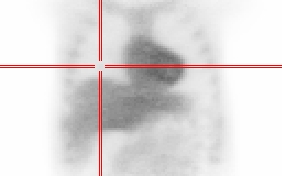
\includegraphics[width=3cm]{images/ite1} & 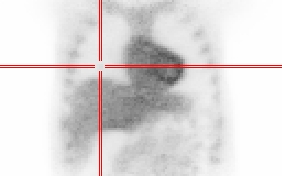
\includegraphics[width=3cm]{images/ite3} & 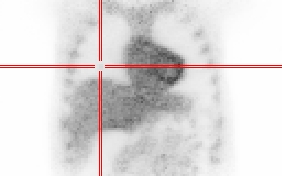
\includegraphics[width=3cm]{images/ite5} & 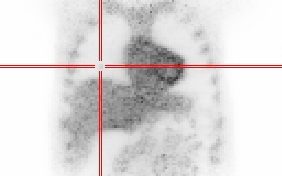
\includegraphics[width=3cm]{images/ite7} \\
Itération 1  & Itération 3 & Itération 5 & Itération 7 \\
\hline
 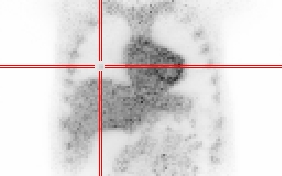
\includegraphics[width=3cm]{images/ite9} & 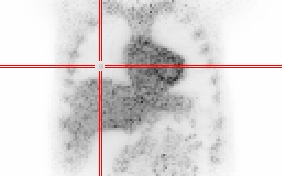
\includegraphics[width=3cm]{images/ite11} & 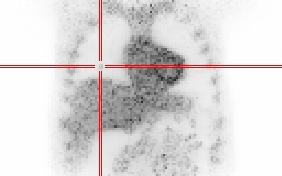
\includegraphics[width=3cm]{images/ite13} &  \\
Itération 9  & Itération 11 & Itération 13 &\\
\end{tabular}

\caption[Illustration de l'évolution des lésions en fonction du nombre d'itérations]{Illustration de l'évolution des images en fonction du nombre d'itérations utilisées pour la reconstruction. Une lésion est présente au centre de la croix rouge.}
\label{fig:evolRecon}
\end{figure}

L'optimisation du nombre totale d'itérations est réalisée en maximisant le rapport contraste sur bruit~\cite{takahara2004diffusion} (CSR) des lésions, défini comme suit :

\begin{equation}
 CSB = \frac{µ_{signal} - µ_{fond}}{\sqrt{\sigma_0}}
\end{equation}

Où $µ_{signal}$ et $µ_{fond}$ représentent, respectivement, l'activité moyenne d'une zone d'intérêt de taille 3$\times$3$\times$3 voxels centrée sur une lésion, et l'activité moyenne d'une zone saine. Cette zone correspond à un volume de 200 voxels dans le poumon et de 64 voxels dans le foie. $\sigma_0$ représente la variance du bruit. Dans notre cas, cette variance est évaluée sur la zone saine utilisée précédemment. Appliquée aux lésions, cette métrique a l'avantage de permettre une représentation rapide de l'évolution du contraste entre la lésion et le fond, tout en pénalisant le bruit.

L'évaluation du rapport contraste sur bruit est réalisée sur une acquisition statique d'un modèle de patient contenant 12 lésions (6 dans le foie et 6 dans le poumon), de diamètre et de contraste échantillonnés à partir des valeurs calibrées dans la table \ref{tab:contrastePoumonFoieRecap} présentée à la page \pageref{tab:contrastePoumonFoieRecap}.

Les résultats sont présentés dans la figure \ref{fig:CNRFoie} pour le foie et \ref{fig:CNRPoumon} pour le poumon.

\begin{figure}
\centering
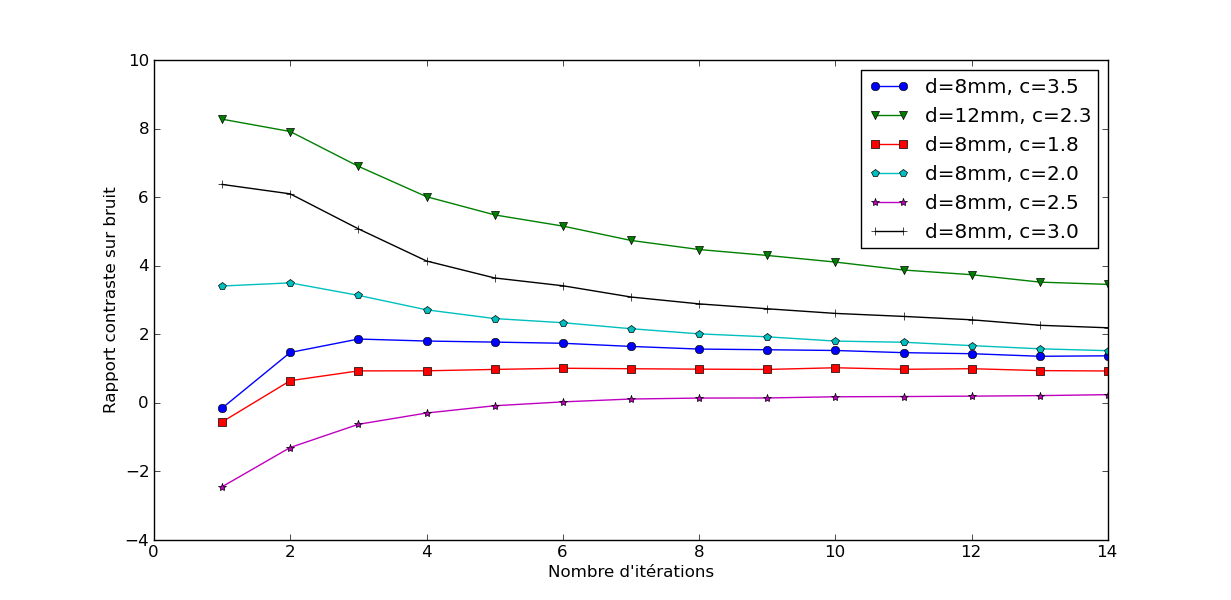
\includegraphics[width=17cm]{images/CNRFoie}
\caption[Evaluation du rapport contraste sur bruit des lésions du foie en fonction du nombre d'itérations]{Evaluation du rapport "contraste sur bruit" des lésions du foie en fonction du nombre d'itérations : sont indiqués, pour chaque lésion, le niveau de contraste réel ainsi que le diamètre de la lésion}
\label{fig:CNRFoie}
\end{figure}


\begin{figure}
\centering
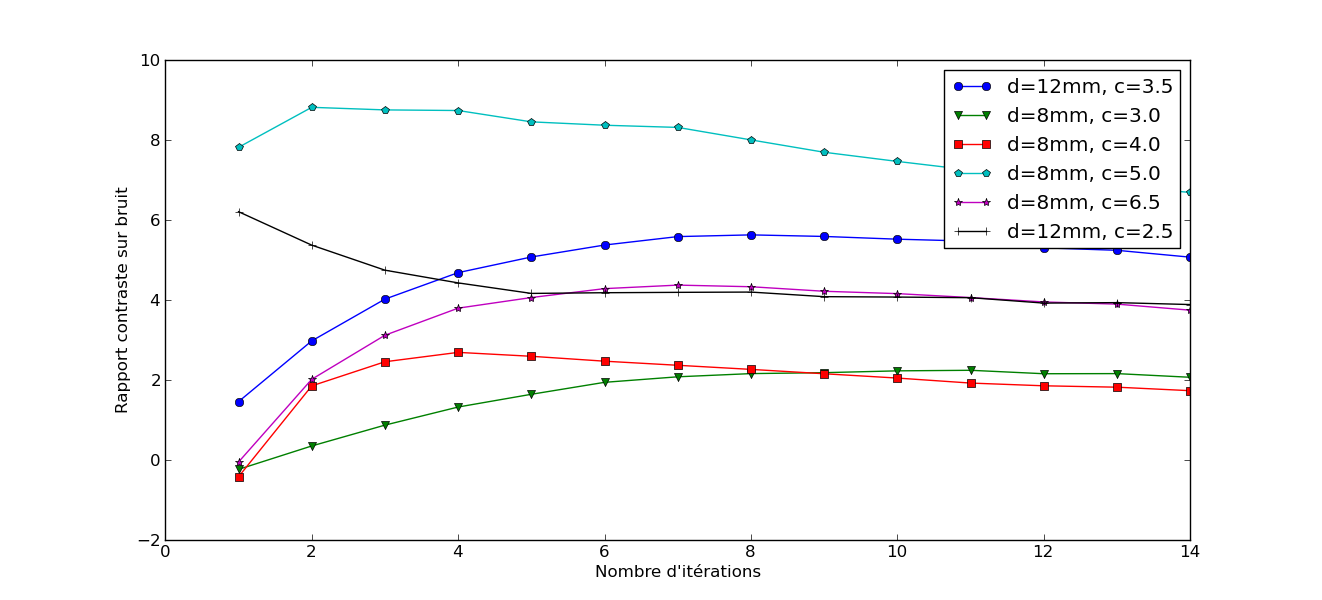
\includegraphics[width=17cm]{images/CNRPoumon}
\caption[Evaluation du rapport "contraste sur bruit" des lésions du poumon en fonction du nombre d'itérations]{Evaluation du rapport Contraste sur bruit des lésions du poumon en fonction du nombre d'itérations : sont indiqués, pour chaque lésion, le niveau de contraste réel ainsi que le diamètre de la lésion}
\label{fig:CNRPoumon}
\end{figure}

La première observation est que certaines courbes sont strictement descendantes, surtout dans le foie. Cela s'explique par le fait que le niveau de bruit augmente beaucoup plus rapidement que la différence d'activité entre le signal et le fond. Cependant, les lésions concernées ont toutes un contraste très élevé, ce qui les rend plus facilement détectables. Par contre, pour les autres, on peut voir que l'optimum du CSR des lésions du foie est situé autour de 4 itérations, suivi par un plateau, tandis que l'optimum du CSR des lésions du poumon est plus proche de 8 itérations complètes.

La lésion du foie ayant un contraste de 2.5 et un diamètre de 8mm a une valeur de rapport contraste sur bruit négative. Cela s'explique par le fait que pour les premières itérations, une faible différence d'activité en faveur du fond peut être fortement accentuée par l'écart type qui est très faible. De la même manière, pour les itérations suivantes, l'activité de cette lésion redevient supérieure à celle du fond, mais l'écart-type du bruit devient plus important, ce qui fait que le rapport est proche de zero. Lorsque le nombre d'itérations est très faible, on observe une diminution de l'activité des petites structures par effet d'étalement (spill-out). Pour des nombres d'itérations plus importants, l'effet de volume partiel diminue, ce qui signifie que l'activité du centre de la lésion augmente.

Nous avons choisi de réaliser les reconstructions avec 8 itérations de 5 sous-ensembles car nous avons montré que ce nombre d'itérations est optimal pour les lésions du poumon, et ne pénalise pas trop la détectabilité des lésions du foie.


%%%%%%%% NE SAIS PAS OU LE METTRE
% \subsection{Gestion des lits}
% 
% Le découpage des simulations en "lits" est nécessaire pour simuler de manière réaliste des acquisitions médicales. En effet, le champ de vue de la caméra PET est très limité, et de l'ordre de quelques dizaine de cm. Le patient est donc déplacé entre chaque acquisition, et chacune de ces positions correspond à un "lit" différent.
% 
% Or le logiciel de reconstruction avec correction de mouvement ne prenait pas en compte la possibilité de découper les images en lits.
% 
% Nous avons donc modifié le logiciel pour permettre la prise en compte de champs de mouvement corps-entier lors de la reconstruction d'un seul lit. En pratique, le lit à recaler est insérée dans un volume de la taille du champ de mouvement, puis ce champ de mouvement est appliqué sur l'image. Le lit est ensuite extrait de l'image déformée pour continuer la reconstruction.


\section{Estimation du mouvement}

L'estimation du mouvement est réalisée uniquement à partir des données TEP et des informations de synchronisation respiratoire. 

\subsection{Principe de l'estimation de mouvement}

L'estimation du mouvement est réalisée selon le principe énoncé en~\ref{lab:estimMvtTEP4D} :
\begin{enumerate}
 \item Les données simulées de chaque partie de cycle sont additionnées pour les N instants du cycle respiratoire.
 %\item Les images correspondant à chaque instant du cycle respiratoire sont reconstruites à partir de ces données en utilisant l'algorithme OPL-EM.
 \item Les N images reconstruites à partir des données précédentes sont utilisées pour calculer le mouvement respiratoire : les images des temps 2 à N sont recalées sur l'image de référence (numéro 1), ce qui associe à chaque instant respiratoire un champ de déformation.
\end{enumerate}


Le champ de mouvement est estimé en utilisant une méthode de recalage par B-splines. Il est représenté par un nombre réduit de coefficients $c$ de fonctions $\beta^n$ placées sur une grille dans le volume, comme présenté dans la figure~\ref{fig:Bspline}. L'implémentation de cet algorithme a été fournie par Philips France (laboratoire Medisys). La transformation $g_t(x)$ utilisée pour associer les images temporelle  $f(x,t)$ (pour t allant de 2 à N) avec l'image de référence $f(x,1)$, est représentée de la manière suivante :

\begin{figure}
\centering
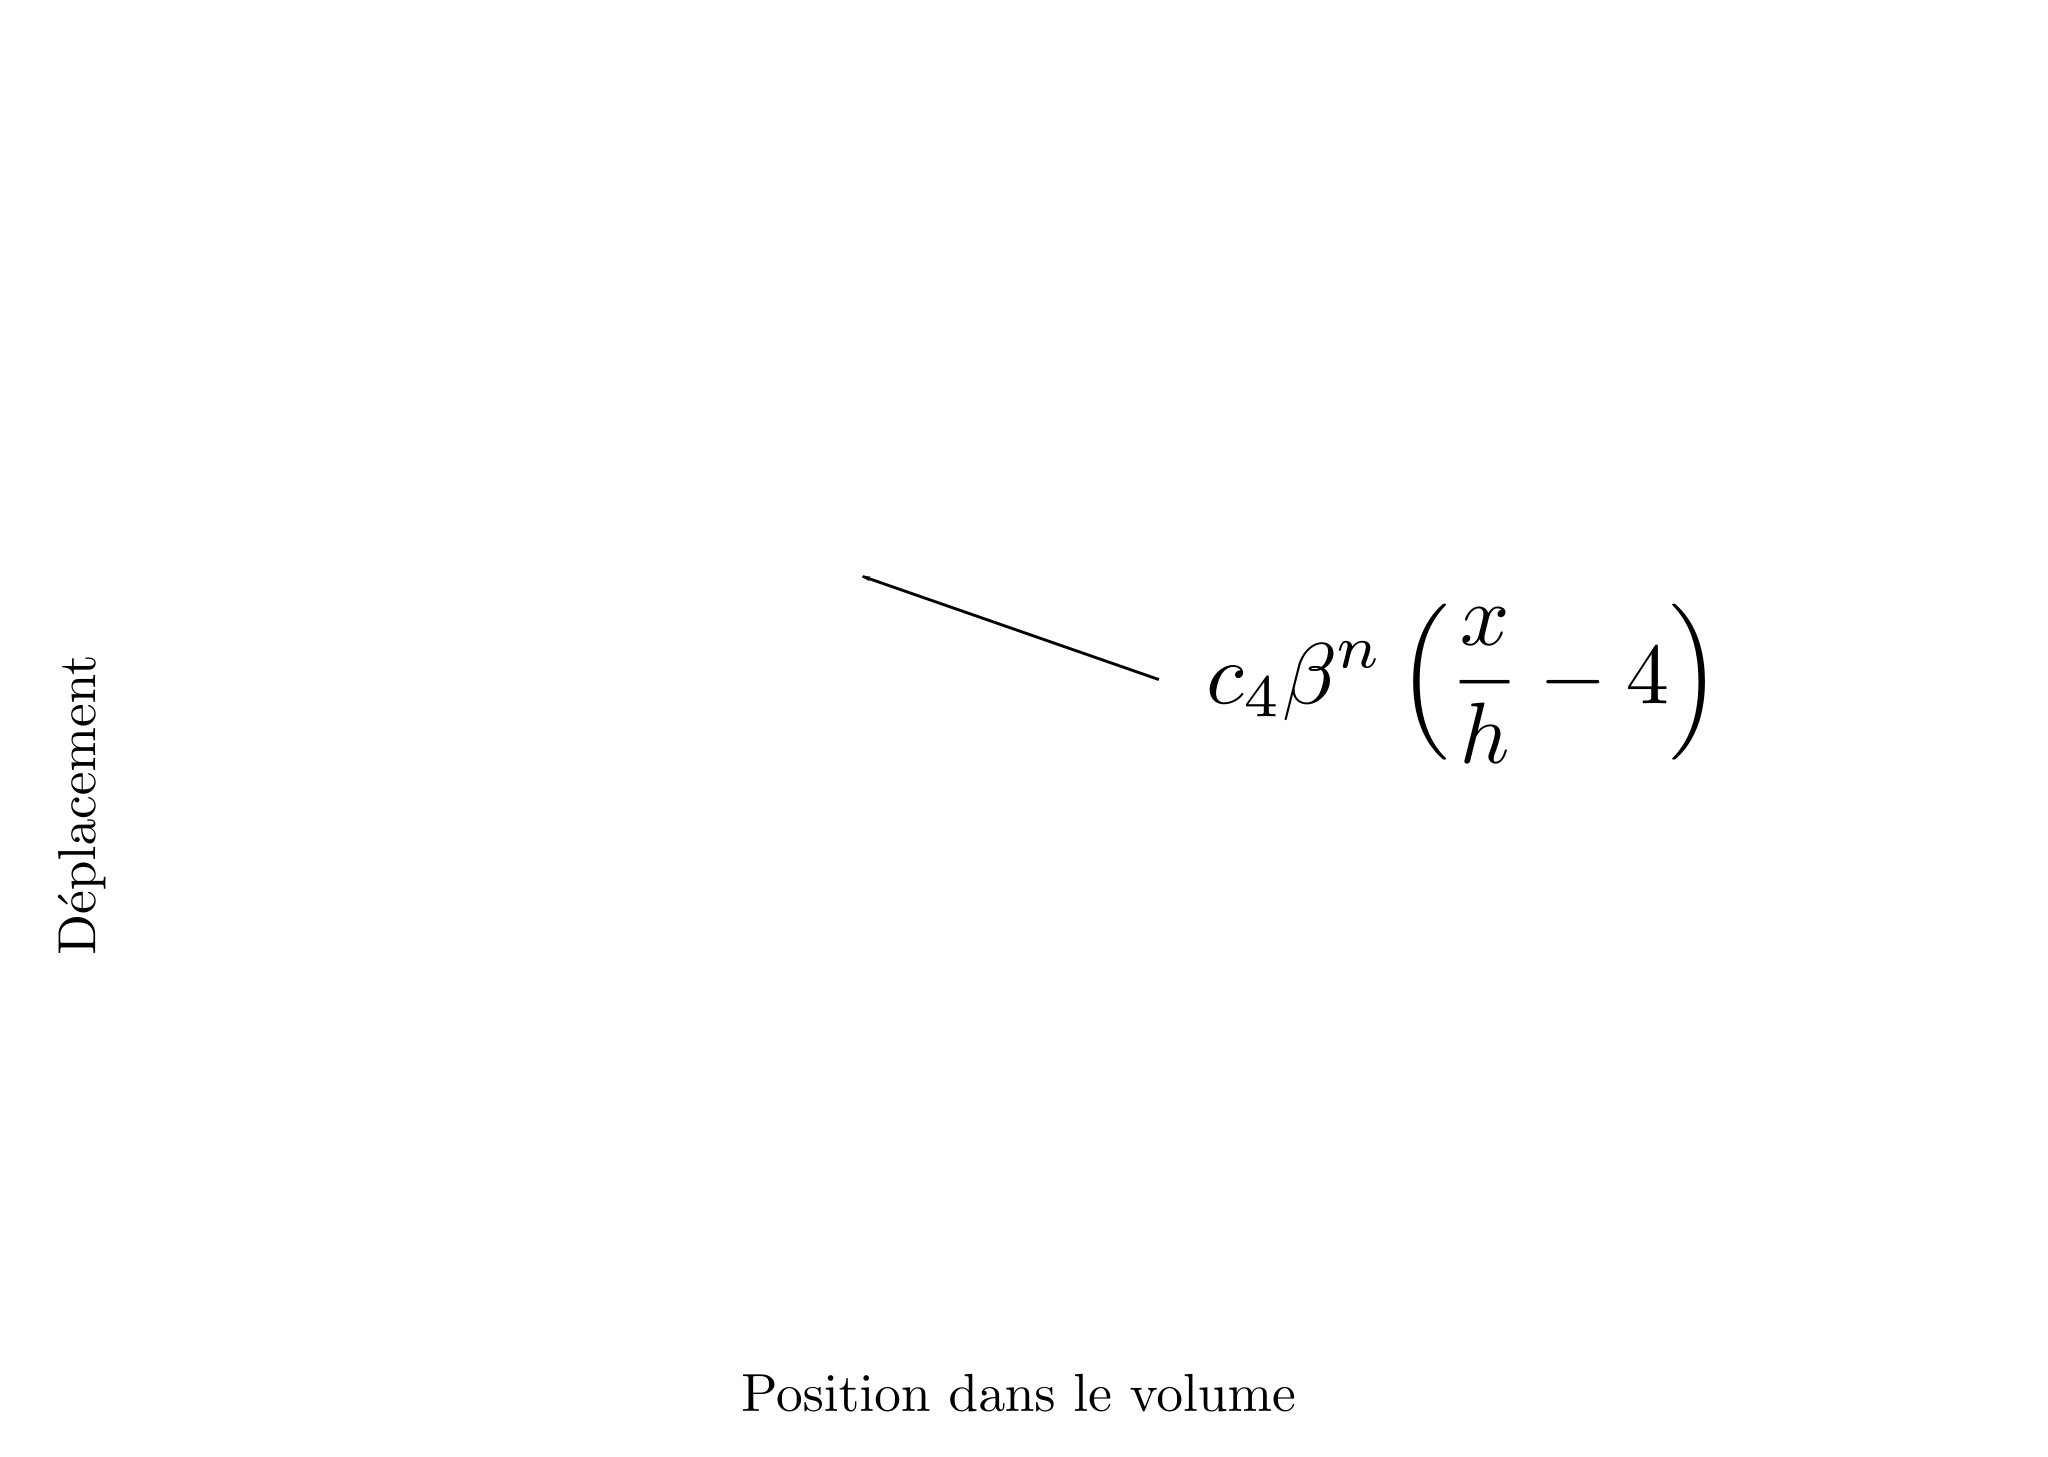
\includegraphics[width=17cm]{images/Bspline}
\caption[Exemple d'interpolation par B-spline]{Exemple d'interpolation par B-spline en 1 dimension : La courbe en trait pointillé épais est représentée par la la somme des contributions des courbes B-spline représentées en traits pointillés fins. Les points de la grille utilisée pour le placement des courbe sont représentés par les ronds rouge.}
\label{fig:Bspline}
\end{figure}


\begin{equation}
  g_t(x)=x + \sum\limits_{j\in \mathbb{Z}^N} c_j \beta^n \left( \frac{x}{h}-j \right)
\end{equation}

Où $\beta^n(x)$ est la valeur de la fonction B-spline de degré $n$ au point $x$, et $j$ représente les indices des positions de la grille. Le paramètre $h$ correspond à l'espacement entre les points de la grille. A chaque fonction B-spline de la grille correspond un coefficient de pondération associé nommé $c_j$ qui représente l'apport de la B-spline correspondante au signal final.

Les coefficients $c_j$ sont obtenus à l'aide d'une optimisation multi-échelle sur 3 niveaux : L'estimation est réalisée sur des images de résolution différente, en se basant sur l'estimation à la résolution $r-1$ pour réaliser celle de l'estimation à la résolution $r$. l'optimisation est réalisée par gradient conjugué selon la méthode de Polak-Ribière~\cite{polak1969note}. Nous avons utilisé l'erreur quadratique moyenne pour comme métrique de recalage. Elle a l'avantage d'être simple, rapide, et de ne pas montrer de discontinuités~\cite{ledesma2005spatio}. Nous avons choisi d'utiliser des splines d'ordre 1.


\subsection{Paramètres de l'estimation de mouvement}

%Les images utilisées pour l'estimation du mouvement respiratoire ne sont pas reconstruites avec les mêmes paramètres que les images finales. En effet, la quantité de données disponible pour la reconstruction est 8 fois plus faible que celle utilisée pour réaliser les reconstructions d'images. De plus, nous cherchons à optimiser la qualité de l'estimation de mouvement. 

Lestimation du champ de mouvement est réalisée à partir des 8 images TEP correspondant aux 8 positions temporelles du cycle respiratoire. Ces données contiennent donc 8 fois moins d'évènements que les images statiques. Ainsi, les paramètres de reconstruction déterminés en~\ref{lab:paramRecon} ne sont pas optimaux pour ces images, d'autant que nous cherchons, à ce stade, à optimiser la qualité de l'estimation de mouvement. C'est pour ces raisons que nous avons réalisé une autre étude pour estimer les paramètres de reconstruction pour cette problématique spécifique. 


\subsubsection{\'Evaluation de l'estimation de mouvement}

Pour évaluer la performance de chaque jeu de paramètre, nous avons utilisé la vérité terrain fournie par la carte de labels pour créer une image d'évaluation correspondant à l'image de référence, ainsi qu'une autre correspondant à l'image ``respirante``. Les images d'évaluation sont créées à partir des fantômes de référence en assignant aux organes étudiés (foie et poumon) une valeur de 1, et une valeur plus importante pour les lésions. Le reste a une valeur de 0. Une illustration est présentée dans la figure~\ref{lab:illustrationRecalage}.a). 

\begin{figure}
\centering
\begin{tabular}{c c}
	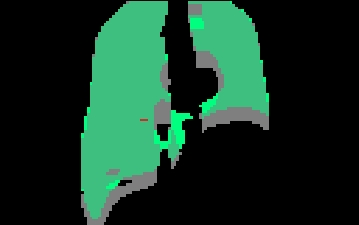
\includegraphics[width=5cm]{images/sansCorrection} & \includegraphics[width=5cm]{images/avecCorrection} \\
	a) Cartes non recalées				& b) Cartes recalées
\end{tabular}
\caption[Illustration du recalage obtenu]{Illustration de la pertinence du recalage obtenu à partir de l'estimation de mouvement réalisée sur les images. En vert l'image de référence et en gris l'image du temps correspondant à la différence la plus importante. }
\label{lab:illustrationRecalage}
\end{figure}

L'image d'évaluation correspondant à l'image ''respirante`` est alors recalée sur l'image de référence à l'aide du champ de mouvement élastique calculé précédemment. Nous évaluons ensuite la qualité du recalage en calculant l'écart quadratique moyen entre les deux images d'évaluation~\ref{lab:illustrationRecalage}.b).

\subsubsection{Optimisation des Paramètres de l'estimateur de mouvement}

Nous avons évalué l'influence de l'échantillonnage spatial des B-spline sur la qualité de l'estimation de mouvement. En effet, si l'espacement entre les nœuds de contrôle est trop important, les mouvements locaux vont interférer entre eux et le résultat ne sera pas valide. De la même manière, en cas d'espacement trop faible, la nature extrêmement bruitée des images va engendrer des micro-mouvements parasites locaux. Pour réduire le bruit, nous appliquons un filtrage gaussien de largeur à mi-hauteur égale à 6 mm à chaque itération.

Nous avons évalué le recalage des reconstructions pour les paramètres suivants :
\begin{description}
 \item[Nombre d'itérations :] Le nombre de sous-ensembles est toujours de 5, mais nous faisons varier le nombre d'itérations de 1 à 7, ce qui représente un nombre d'itérations totales de 5 à 40.
 \item[Précision de la grille :] nous avons évalué les performances de la détection pour 3 taille différentes, allant d'une grille très peu précise de 2 noeuds en x, y et z, à une grille plus précise avec 5 noeuds en x et y, et 10 noeuds en z. Une grille intermédiaire a été évaluée avec 3 noeuds en x et y, ainsi que 5 noeuds en z.
\end{description}

Les résultats sont présentés dans la figure~\ref{fig:perfsFctIterTaille}. Les meilleures performances sont obtenues pour la configuration $3 \times 3 \times 5$ avec 3 itérations et 5 sous-ensembles.

\begin{figure}
\centering
\includegraphics[width=12cm]{images/perfsRecalageFctIter-grid_crop}
\caption[Performances de l'estimation de mouvement en fonction de la taille de la grille de recherche]{Performances de l'estimation de mouvement en fonction du nombre d'itérations de la reconstruction selon la taille de la grille utilisée pour l'estimation de mouvement}
\label{fig:perfsFctIterTaille}
\end{figure}

\subsubsection{Optimisation des paramètres de la reconstruction}

Nous avons ensuite souhaité vérifier que la régularisation avait un impact positif sur la qualité du recalage. Nous avons utilisé les paramètres présentés précédemment pour la valider :

\begin{description}
 \item[Nombre d'itérations :] Le nombre de sous-ensembles est de 5, mais nous faisons varier le nombre d'itérations de 1 à 7, ce qui représente un nombre d'itérations totales de 5 à 40.
 \item[Présence ou absence de régularisation pendant la reconstruction :] Une régularisation par filtrage gaussien de largeur à mi-hauteur de 6 mm est appliquée ou non à chaque itération.
\end{description}

Les résultats sont présentés dans la figure~\ref{lab:perfsFctIterReg}. Ils montrent clairement que la régularisation entraîne une amélioration des performances, et que la meilleure estimation de mouvement est réalisée pour une reconstruction de 3 itérations avec 5 sous-ensembles. Nous avons par conséquent utilisé ces paramètres avec une grille de 3 noeuds en x et en y, soit un espacement de 17cm, et de 5 noeuds en z, soit un espacement de 7.7 cm.

\begin{figure}
\centering
\includegraphics[width=10cm]{images/perfsRecalageFctIter_crop}
\caption[Performances de l'estimation de mouvement en fonction de la régularisation]{Performances de l'estimation de mouvement en fonction du nombre d'itérations complètes de la reconstruction selon la présence ou l'absence de régularisation pendant la reconstruction. Plus la valeur en ordonnées (mesure de différence) est faible, meilleure et la performance}
\label{lab:perfsFctIterReg}
\end{figure}


\section{Méthodes de correction du mouvement respiratoire}

Nous avons choisi de corriger les images TEP en utilisant la méthode de correction post reconstruction décrite en \ref{lab:corrPostRecon} ainsi que la correction par modification de la matrice système décrite en \ref{lab:corrMatSyst}. La première est déjà implémentée sur les imageur GE (technologie motionFree), tandis que la seconde est activement étudiée en recherche. Des images générées sur deux patients sont présentées dans la figure~\ref{fig:exempleImageReconTous}.

Les images ont été reconstruites à l'aide de l'algorithme OPL-EM. L'implémentation de cet algorithme a été développé par le Laboratoire de Traitement de l'Information Médicale de Brest (LATIM)\cite{lamare2007list}. L'implémentation permet de prendre en compte la correction de l'atténuation, mais ne permet pas la correction des coïncidences aléatoires et des coïncidences diffusées. Nous avons donc choisi de simplifier le problème en supposant une correction parfaite de ces deux effets. Pour cela, nous n'avons pas inclus les photons diffusés ou les coïncidences aléatoires dans les données séquence. 


\begin{figure}
 \centering
 \includegraphics[width=15cm]{images/exempleImageReconToutes}
 \caption[Exemples d'mages reconstruites corrigées et non corrigées du mouvement]{Images reconstruites avec et sans correction du mouvement respiratoire (8 itérations et 5 subsets). Les flèches représentent une lésion du foie de diamètre 8 mm avec un contraste de 3.5 dans le patient 1, ainsi que deux lésions du poumon de 8 mm et de contraste 6.5 pour le patient 2.}
 \label{fig:exempleImageReconTous}
\end{figure}


\subsection{Images Statiques}

Les images statiques sont reconstruites à partir des donnés de simulation statiques, réalisées à partir d'une acquisition complète du modèle au premier instant du cycle respiratoire (fin d'expiration).

Chaque image est donc en phase avec la carte d'atténuation qui est elle aussi tirée du modèle en fin d'expiration. Les images ont été reconstruites à l'aide de l'algorithme OPL-EM avec 8 itérations comprenant 5 sous-ensemble chacune.

\subsection{Images Non corrigées}

Les images non corrigées sont produites de la même manière que les images statiques, mais à partir des fichiers séquence dynamiques. Ces fichiers correspondent à une acquisition en respiration libre de 224 secondes. 

La carte d'atténuation utilisée est celle correspondant au premier instant du cycle respiratoire.

\subsection{Images TE-MS}

Ces images sont reconstruites en utilisant la méthode décrite en~\ref{lab:CorrpendantRecon}, qui prend en compte l'estimation de mouvement réalisée précédemment ainsi que les fichiers séquence générés par la simulation dynamique pour reconstruire directement les images corrigées. 

La carte d'atténuation de l'instant de référence est déformée à l'aide des champs de mouvements pour générer 8 cartes d'atténuation. Les données de chaque instant du cycle respiratoire seront corrigées avec la carte d'atténuation correspondante.

\subsection{Images TE-IM}

La méthode TE-IM est présentée en~\ref{lab:corrPostRecon}. Les 8 images correspondant aux 8 instants du cycle moyen sont reconstruites séparément à l'aide de la carte d'atténuation recalée correspondante. Chacune de ces image est recontruite avec les mêmes paramètres que pour les autre types d'images, soit 8 itérations et 5 subsets. Ces 8 images sont ensuite déformées sur l'image correspondant au premier instant du cycle, à l'aide de la carte de mouvement estimée précédemment. Ces 8 cartes recalées sont ensuite sommées pour obtenir les images corrigées.

Bien que chaque image prise indépendamment soit très bruitée à cause du faible nombre d'évènements, la déformation suivie par la sommation des différentes images apporte une régularisation importante, comme on peut le voir dans la figure~\ref{fig:exempleImageReconTous}. 

\section{Système CAD} % 11.1

Le système CAD que nous utilisons a été développé à l'origine pendant les travaux de thèse de Sandrine Tomeï ainsi que mes travaux de master~\cite{tomei2008automatic,lartizien2010impact}. Nous l'avons amélioré et adapté aux besoins de cette étude, notamment en développant les mesures de performances.


Le CAD utilise des informations fréquentielles obtenues par décomposition des images en ondelettes biorthogonale 4/4 non décimée (figure \ref{fig:ondelettes}) . Ces données sont utilisées par le système de classification basé sur un SVM travaillant voxel par voxel. Une étape de réduction des faux positifs est ajoutée par la suite.

Le nombre de tumeurs utilisées pour générer la base d'apprentissage est de 107 pour la base d'apprentissage poumon et 173 pour la base d'apprentissage foie. Ce nombre est relativement faible~\cite{hua2005optimal} par rapport à la taille du vecteur de caractéristiques utilisé pour le CAD (entre 24 et 32), ce qui nécéssite de prendre en compte un maximum de données pour l'apprentissage et le test pour éviter le sous-apprentissage. Nous avons donc utilisé une méthode d'évaluation des performances par resubstitution. Cela signifie que les apprentissages et les tests sont réalisés sur la même base de données constituée de 15 patients présentés dans le chapitre 10. %\ref{lab:bdd}.

\subsection{Vecteur de Caractéristiques}

Nous avons choisi d’utiliser une décomposition en ondelettes 3D non décimées par banc de filtres. Dans le cas tridimensionnel, la décomposition par banc de filtres est résumée par la figure \ref{fig:ondelettes}. L’image de départ est traitée successivement dans les trois directions de l’espace par un filtre fréquentiel passe-haut correspondant à la fonction d’ondelettes (noté $H$) et passe-bas correspondant à la fonction d’échelle (noté $L$). 

\begin{figure}
 \includegraphics[width=15cm]{images/decompHotell}
 \caption[Décomposition en ondelettes par banc de filtres]{Décomposition en ondelettes par banc de filtres : Chaque image est filtrée selon les 3 dimensions pour obtenir les coefficients d'ondelettes et d'échelle de chaque voxel de l'image. L correspond à un filtrage passe-bas tandis que H correspond à un filtrage passe-haut. Les coefficients d'échelle sont contenus dans l'image $LLL_{j+1}$ tandis que les coefficients d'ondelettes sont présents dans les sept images de détail $LLH_{j+1}$, $LHL_{j+1}$ \dots $HHH_{j+1}$ }
 \label{fig:ondelettes}
\end{figure}

\begin{figure}
 \centering
 \includegraphics[width=15cm]{images/exemplesDecomp}
 \caption[Exemples de décomposition d'images en ondelettes]{Exemples d'images TEP décomposées en ondelettes. Sont représentées l'image originale, puis l'image des coefficients d'échelle notée $LLL_j$ et une image des coefficients d'ondelettes notée $HHH_j$ pour deux niveaux de décomposition. L'ondelette utilisée pour la décomposition est la biorthogonale 4/4}
 \label{fig:bior44Ex}
\end{figure}


Ainsi sept images de détails (HHH, LLH, \dots) et une image d’approximation (LLL) sont produites pour chaque niveau $j$ de décomposition. Les huit images du niveau suivant $j+1$ sont générées de la même manière, mais en considérant l’image d’approximation $LLL_j$ du niveau précédent comme image de départ. Les caractéristiques des images, rassemblées dans un vecteur descripteur de taille $8 \times j$, correspondent ici à l’ensemble de ces coefficients pour chaque voxel  de l’image. Des exemples d'images obtenues par les filtrages sont présentés dans la figfure \ref{fig:bior44Ex}.

Nous utilisons l'ondelette biorthogonale 4/4 dont la fonction est présentée sur la figure \ref{fig:bior44}.


\begin{figure}
 \begin{tabular}{ c c }
 
 \includegraphics[width=8cm]{images/bior44Ondelette} & \includegraphics[width=8cm]{images/bior44Echelle} \\
 Fonction d'ondelette & Fonction d'échelle\\
 \end{tabular}

 \caption{Fonction d'ondelette et d'échelle biorthogonale 4/4}
 \label{fig:bior44}
\end{figure}

\subsection{Génération de la base d'apprentissage}
Les données générées par la décomposition en ondelettes de chaque image se présentent sous la forme de volumes 4D, indiquant pour chaque voxel de l'image 3D l'ensemble des $8 \times j$ coefficients associés.

La base d'apprentissage sert à entraîner le classifieur dans un processus de classification supervisée, en lui fournissant un ensemble d'exemples avec leur classes associées (voir figure \ref{fig:fonctClassif}) page \pageref{fig:fonctClassif}).

La génération de cette base demande l'extraction de points de la classe ``pathologique'', et de la classe ``sain''. Pour chaque tumeur de la vérité terrain, nous extrayons de l'image correspndante le vecteur de caractéristiques du voxel placée au centre de la tumeur. Ce vecteur de caractéristique correspond aux coefficients de la décomposition en ondelette du voxel de l'image ($8 \times j$).

Les points de la classe ``sain'' sont extraits de manière aléatoire dans les volumes de toutes les images (hors tumeurs). Pour des raisons de simplicité d'implémentation, un nombre fixe de points est extrait de chaque image.

\subsection{Apprentissage de la Machine à Vecteur de Support (SVM)}

La base de données d'apprentissage est utilisée  par le classifieur SVM (Machine à Vecteur de Support) pour l'apprentissage.

Le principe des SVM est de trouver l’hyperplan optimal de séparation dans l'espace des caractéristiques, qui va maximiser la marge de séparation entre les deux classes ``pathologique''  et ``sain'' (le SVM est défini plus en détail en \ref{lab:SVM}). Cette marge correspond à la distance entre les plus proches vecteurs de caractéristiques appartenant à chacune des classes et l'hyperplan. La définition de cette marge et donc de l’hyperplan, se fait uniquement à partir de vecteurs de support, qui correspondent à l'enveloppe du groupement de point de chacune des deux classes.

Le SVM va calculer un modèle décrivant l'hyperplan permettant de séparer les données.

\subsection{Génération des sites présumés}
\label{lab:aggregatsCAD}
Une fois le classifieur entraîné, il est capable de classer rapidement les nouveaux vecteurs de caractéristiques. Ainsi, on lui soumet les données correcpondants aux voxels des images pour qu'il les classe. On obtient donc en sortie un ensemble de cartes de score (une par image 3D), dans lesquelles chaque voxel correspond au score indiqué par le SVM. Ce score est une mesure de distance polarisé par rapport à l'hyperplan de séparation dans l'espace des points d'apprentissage, et donne en plus de la classe, donc une mesure de la ``certitude'' du SVM vis-à-vis de sa classification.

Cette carte de score est ensuite seuillée pour fournir une carte binaire, indiquant pour chaque voxel la classe sélectionnée par le SVM pour ce niveau de seuil. Le mécanisme de sélection du seuil est défini en \ref{lab:selectionSeuil}. Une exemple de carte de score est visible dans la figure \ref{fig:cheminementCAD}.a.
	
\`A cette étape, le résultat est sous forme d'une carte de voxels étiquetés comme ''sain`` ou ''pathologiques``. Nous avons choisi de travailler sur des agrégats de points plutôt que directement sur les voxels car les cartes binarisées sont relativement bruitées (voir \ref{fig:cheminementCAD}.b), et donc non directement exploitables. Les voxels ``pathologiques'' sont donc regroupés selon une 26-connexité (3x3x3). Un score est associé à chaque  agrégat, correspondant au score le plus important observé dans l'agrégat.

\subsection{Règles d'évaluation du résultat}
\label{lab:reglesSelect}
Pour évaluer le résultat, nous avons élaboré des règles permettant de classer les agrégats à l'aide de la vérité terrain. Ce sont ces algorithmes qui sont utilisés dans les évaluateurs de performances présentés ci-après.

Les agrégats sont classés en LL (Lésion localisée) et NL (Non Lésion) selon qu'ils peuvent être considérés comme des vrais positifs ou des faux positifs :

Soit $\mathbf{L}$ l'ensemble des points de la lésion, $\mathbf{A}$ les points correspondant à l'amas candidat.

Les agrégats seront considérés comme des vrai positifs si ils intersectent une tumeur selon les règles décrites ci-après, ou comme de faux positifs dans le cas contraire. Cependant, si leur taille est inférieure à la taille minimale définie par la première règle, l'amas n'est pas considéré.

Règles de classification :
\begin{enumerate}
 \item $card( \mathbf{L} \cap \mathbf{A} ) > \alpha \times card( \mathbf{L} )$ : où $\alpha$ qui définie la proportion minimale de la tumeur qui doit être présente dans l'amas. Elle permet d'éviter les amas qui intersecteraient la tumeur par accident.
 \item $card( \mathbf{L} \cap \mathbf{A} ) > \beta \times card( \mathbf{A} )$ : où $\beta$ qui limite l'étendue de l'amas en dehors de la tumeur.
\end{enumerate}

$\alpha$ et $\beta$ sont des constantes empiriques fixées respectivement à 0.05 et 0.20 dans nos travaux. Nous avons choisi ces valeurs en visualisant les cartes de score pour obtenir des résultats correctes sans pénaliser les performances.

\subsection{Résumé}

Ce pseudo-code décrit les différentes étapes du CAD, depuis l'importation des images jusqu'à à l'extraction des lésions potentielles. Il est illustré par la figure \ref{fig:cheminementCAD} :

\begin{figure}
 \centering
 \includegraphics[width=15cm]{images/cheminementCAD}
 \caption[Schéma du système CAD]{Schéma du système CAD : l'image d'origine en haut à gauche est utilisée par le classifieur pour générer la carte de score. Cette carte est ensuite seuillée par l'étape b) pour générer une carte binaire correspondant aux sites qui dépassent un certain score $s$. L'étape c) correspond à la formation des agrégats qui seront le résultat du système CAD. Cette étape s'accompagne d'une suppression des sites de trop petite taille. Les flèches représentent des lésions dans l'image d'origine}
 \label{fig:cheminementCAD}
\end{figure}

\begin{enumerate}
 \item Décomposition des images en ondelettes : pour chaque voxel de l'image d'origine, on obtient entre 8 et 32 coefficients suivant le niveau de décomposition de l'image, qui correspondent au vecteur de caractéristiques utilisé par le classifieur.
 \item Extraction de la base d'apprentissage : les coefficients des centres de toutes les tumeurs sont extraits des volumes décomposés, et vont former la base d'apprentissage pathologique. Un certain nombre de voxels sont tirés aléatoirement dans les zones normales de chaque image et leurs coefficients sont ajoutés à la base saine.
 \item Apprentissage : le classifieur SVM est entraîné sur cette base d'apprentissage pour générer le modèle qui sera utilisé pour le test.
 \item Tests : le SVM entraîné est utilisé pour classer chaque voxel contenu dans les organes à évaluer (poumon et foie).
 \item Réduction des faux-positifs : les points sont agrégés en composantes connexes (26-connexité en 3 dimensions).
 \item Évaluation : lorsque nous avons accès à la vérité terrain, il est possible d'évaluer les performances du CAD en classant les agrégats en LL (Lésion Localisée) et LN (Lésion Non Localisée).
\end{enumerate}



\section{Optimisation des paramètres du système CAD} % 11.2
\label{lab:optim}

Les différentes étapes de l'évaluation des performances nécessitent de fixer un grand nombre de paramètres que nous allons détailler dans cette partie.

\subsection{Paramètres à optimiser} % 11.2.1
\label{lab:optimParametres}

\subsubsection{Paramètres de la base d'apprentissage}

Nous avons identifié plusieurs autres paramètres qui, sont suceptible d'influencer les performances de détection :

\begin{enumerate}
 \item \textbf{Normalisation :} Le but de la normalisation est d'homogénéiser les plages de valeurs des différentes caractéristiques pour faciliter le travail du classifieur, dont les paramètres $C$ et $\gamma$ (définis ci-après) dépendent de la distance entre les points et ne permettent pas de gérer des différences trop importantes d'étendues dans les caractéristiques.  Nous avons proposée de comparer deux méthodes de normalisation. La première consiste à modifier les données pour que la moyenne et l'écart-type aient une valeur respectivement de 0 et 1 ($(\mu, \sigma)=(0,1)$). Cette méthode est notée ``\emph{moyenne}'' dans la suite du texte. La seconde méthode consiste à adapter des données pour que l'ensemble des valeurs soit comprises entre -1 et +1. Cette méthode est notée ``\emph{écart}''. La première méthode (\emph{moyenne}) a l'avantage d'être relativement peu sensible aux valeurs extrêmes, contrairement à la seconde (\emph{écart}).


 \item \textbf{Nombre de points de la base d'apprentissage :} Le nombre de point de la base d'apprentissage détermine directement la qualité du modèle. Le nombre de caractéristiques de chaque exemple de la base est de $8 \times j$, avec $j$ le niveau de décomposition des images. Il n'existe pas de règle définitive pour choisir le nombre d'exemples nécessaires en fonction du nombre de caractéristiques, mais l'on considère cependant que le nombre d'échantillons de la base d'apprentissage doit être largement supérieur au nombre de caractéristiques pour éviter le sur-apprentissage. Cependant, les SVM sont relativement efficaces pour éviter ce problème. Dans notre étude, le nombre de cas pathologiques est de 173 pour le poumon et de 107 pour le foie. Il faudrait idéalement sélectionner autant de cas ``sains'' que de cas pathologiques pour chaque organe. Cependant le nombre total de cas risque d'être trop faible par rapport au nombre de caractéristiques. Nous avons par conséquent analysé l'influence du nombre de cas sur les performances de détection en considérant trois valeurs : 100 points normaux par images (pts/im.) (soit 1500 pts. négatifs), 200 pts/im. (soit 3000 pts. négatifs) et 1000 pts/im. (soit 15000 pts. négatifs).


 \item \textbf{positions des points extraits :} Les points normaux extraits des images pour alimenter la base vont avoir une influence directe sur la qualité des résultats. Idéalement ils devraient être représentatifs de l'ensemble des cas rencontrés dans la base de tests, néanmoins les bords de certains organes ont un profil proche de celui des tumeurs, et rendent l'estimation de la surface de séparation plus difficile. Nous avons donc voulu évaluer la performance du CAD sur une base dépourvue de ces données ambiguës. Pour cela nous avons réalisé une érosion de 2 voxels sur les masques des volumes sains à extraire, afin de ne pas prendre en compte les frontières des organes.
\end{enumerate}



\subsubsection{Paramètres du classifieur}
\label{lab:paramClassif}
Le classifieur (SVM) utilise les données d'apprentissage formatées selon les choix opérés précédemment (normalisation, volumes utilisés pour extraire les points de la base de points ''sain`` et nombre de ces points) pour générer un modèle de prédiction. Cependant, cet algorithme dispose de paramètres intrinsèques, qui sont beaucoup plus dépendant des données d'apprentissage(voir \ref{lab:SVM}).

\begin{description}
 \item[Niveau de la décomposition en ondelettes $j$ :] Ce paramètre détermine la taille du vecteur de caractéristiques. il correspond au nombre de niveaux de décomposition pris en compte par le SVM. Les niveaux de décomposition élevés ($j$ grand) correspondant à des informations de très basse fréquence, les informations qu'ils apportent ne sont pas forcément pertinentes pour la détection des lésions. Cependant, les caractéristiques fréquentielles des images générées par les différents jeux d'images étant différentes, il est nécessaire d'adapter ce paramètre à chaque type d'images.
 \item[Coefficient de pénalisation $C$ :] lors du calcul de l'hyperplan de séparation des données, chaque point mal classé va pénaliser la surface selon un facteur proportionnel à $C$, comme indiqué en~\ref{lab:SVM}.
 \item[Largeur de bande $\gamma$ :] cette valeur influe directement la largeur de bande du noyau utilisé par le classifieur (Fonction de Base Radiale gaussienne, ou RBF). Voir la description du SVM en~\ref{lab:SVM}
\end{description}

\subsection{Méthodes d'optimisation}
\label{lab:optimCGJ}

Pour chaque combinaison des paramètres de la base d'apprentissage définis en~\ref{lab:paramClassif}, nous avons déterminé le triplet optimal de paramètres ($C$, $\gamma$, $j$) à l'aide d'une recherche exhaustive par grille. Cela correspond à évaluer les performances sur le produit cartésien d'une discrétisation des valeurs de chaque paramètre. Cette étude a été réalisée sur le jeu d'images statiques afin de ne pas être influencé par les éventuels artefacts des autres types d'images.

Par exemple, si nous disposons de deux paramètres A et B, et que nous recherchons le meilleur jeu de paramètres, il faut tout d'abord sélectionner pour chaque paramètre la taille de la zone de recherche. Supposons par exemple que les valeurs de A soient des valeurs entières comprises entre -1 et 2, et que B puisse prendre les valeurs 100, 10000 et 50000. Les critères de performance seront évalués pour toutes les combinaisons des valeurs de A et B, tels que (-1, 100), (-1, 10000), (-1, 50000), (0, 100), \dots, (2, 50000). Le jeu de paramètres ayant obtenu les meilleures performances sera donc sélectionné. 

Les critères de performance que nous avons sélectionnés sont la sensibilité et la spécificité obtenue pour une validation croisée à 5 éléments réalisée sur la base d'apprentissage comme présenté sur la figure \ref{fig:crossValid}. La validation croisée permet de réduire le biais sur les performances~\cite{varma2006bias}.

\begin{figure}[h!]
 \includegraphics[width=15cm]{images/crossValid}
 \caption[Réalisation d'une validation croisée à $n$ éléments]{Réalisation d'une validation croisée à $n$ éléments (ici 4) : La base d'exemples d'origine est décomposée en $n$ parts égales. La mesure de performance se fait $n$ fois, avec à chaque fois un apprentissage sur $n-1$ éléments et un test sur l'élément restant. La mesure de performance est réalisée sur les résultats des $n$ tests.}
 \label{fig:crossValid}
\end{figure}


Pour choisir les meilleurs paramètres du classifieur, j'ai effectué une recherche exhaustive par grille avec les paramètres suivants :

\begin{description}
 \item [$C$ :] de 1 à 10000 en 15 pas logarithmiques
 \item [$\gamma$ :] de 0.0001 à 1 en 15 pas logarithmiques
 \item [$j$ :] de 1 à 4, soit de 8 à 32 caractéristiques
\end{description}

L'optimisation a été réalisée à l'aide du logiciel rapid-i~\cite{mierswa2006} pour chaque type d'image. Les indicateurs de performance calculés par validation croisée sont les suivants : sensibilité, spécificité et précision définis dans le chapitre 7 (section \ref{lab:pressensib}). Le triplet de paramètres retenu est celui qui maximise la sensibilité.

Nous avons représenté pour chaque jeu d'image le nuage de points correspondant à la répartition de chaque triplet ($C, \gamma, j)$ dans un espace à deux dimensions (``Sensibilité'', ``Spécificité''). De ce nuage de points nous pouvons voir le front de Pareto. Ce type de diagramme permet de rechercher un optimum selon plusieurs critères antagonistes. Dans notre cas, nous voulons à la fois une sensibilité et une spécificité importante, sachant qu'il n'existe pas de jeu de paramètres ''parfaits`` qui permettent d'avoir 100\% aux deux. Dans notre cas, le front de Pareto va permettre de vérifier que le choix par maximisation de la sensibilité ne se fait pas au détriment de la spécificité.


\subsection{Mesure de performances de détections}
\label{lab:selectionSeuil}
\label{lab:optimIMSTNOMS}
Les performances de détection obtenues par la méthode de validation croisée considère uniquement le voxel central de la tumeur
pour déterminer si la lésion est correctement détectée. Ces performances ne traduisent donc pas forcément le comportement d'un observateur humain, qui détecte plutôt des aggrégats. Nous avons donc proposé d'estimer les performances en considérant la notion d'aggrégats. Pour un seuil donné, le CAD génére un ensemble d'agrégats associés à un score, comme présenté en \ref{lab:aggregatsCAD}. Il est ensuite possible d'évaluer la performance de ce CAD à l'aide de courbes F-ROC décrites en \ref{lab:FROC} construites à l'aide de la vérité terrain.

Le seuil sélectionné $s$ pour générer les agrégats est celui qui maximise la Fraction de Localisation de Lésion (FLL : nombre de lésions localisées divisé par le nombre total de lésions), c'est à dire celui qui va permettre de détecter un maximum de lésions. 

Cette sélection est réalisée selon l'algorithme suivant :

Le processus d'estimation de la sensibilité pour un seuil $s$ se fait de la manière suivante. Les cartes de scores sont binarisées en fonction de $s$. Les agrégats sont estimés sur ces cartes binaires, en prenant en compte les informations provenant des cartes de score correspondantes pour attribuer un score à chaque agrégat. Ils sont ensuite classés en ''Lésion localisée`` (LL) ou ''Non Lésions`` (NL) à l'aide de la vérité terrain, selon les règles présentées en \ref{lab:reglesSelect}. Une valeur de sensibilité est calculée à partir de ces informations pour le seuil $s$.

Le seuil optimal retenu est celui qui maximise la sensibilité. Nous recherchons ce maximum pour 40 valeurs réparties de manière uniforme entre -2 et +2. Nous utilisons une recherche exhaustive car le résultat possède de nombreux minima locaux et le temps de calcul est faible (moins d'une heure pour les 40 valeurs).

Ce critère de sélection va naturellement engendrer un grand nombre de faux positifs, mais il faut garder à l'esprit qu'il sera utilisé pour réaliser des courbes F-ROC, qui indiquent une spécificité pour chaque nombre de faux positif en jouant sur un second seuil, toujours supérieur à celui retenu pour extraire les agrégats.

Le second critère utilisé pour comparer les bases d'apprentissage est la figure de mérite extraite de l'analyse JAFROC décrite en \ref{lab:AFROC}. Elle va comparer pour chaque image le score du faux positif le plus haut avec les score des vrais positifs de l'image. Pour cette étude, nous avons utilisé la version 4.0 du logiciel JAFROC.

\section{Comparaison des performances de détection des différentes méthodes de correction du mouvement respiratoire}

L'optimisation des paramètres décrits dans la section~\ref{lab:optimParametres} nous a permis de fixer les paramètres de la base d'apprentissage (normalisation, nombre de cas sains, localisation des cas sains).

Afin de comparer les performances des quatre séries (statique, non corrigéee, TE-IM et TE-MS) nous avons dans un premier temps réalisé une nouvelle optimisation des paramètres ($C$, $\gamma$, $j$) pour chaque type d'images en suivant la méthode décrite en~\ref{lab:optimCGJ}. Puis nous avons comparé les courbes F-ROC et réalisé une étude JAFROC comme décrit dans la section~\ref{lab:optimIMSTNOMS}



%%% CHAPITRE 12


\chapter{Analyse des résultats}

Dans ce chapitre nous détaillons les performances de détection obtenus par les quatre séries d'images que nous avons comparées : 'TE-IM; TE-MS, Statiques et Non Corrigées. Nous commençons par présenter les courbes obtenues lors de l'étape d'optimisation et d'adaptation du CAD aux données, puis nous parlons des performances de détection obtenues par ce CAD sur les lésions hépatiques et pulmonaires.

Dans tous les cas, l'estimation des performances se fait de la manière suivante :

\begin{itemize}
 \item Optimisation des paramètres du classifieur au jeu de données.
 \item Comparaison des courbes Free-ROC.
 \item Comparaison des Figures de Mérite JAFROC.
 \item Conclusion
\end{itemize}


\section{Optimisation des paramètres}

Nous avons réalisé des mesures de performances pour les différentes valeurs des paramètres suivants :

\begin{itemize}
 \item Nombre de points de la base d'apprentissage (100, \textbf{200}, 1000)
 \item Normalisation des données (\textbf{moyenne}, écart)
 \item Position des points de la base d'apprentissage (\textbf{organe complet}, organe avec érosion)
\end{itemize}

La recherche des paramètres optimaux a été réalisée sur le foie, pour la série d'images statiques, afin de ne pas être influencé par les artefacts des méthodes de correction du mouvement respiratoire. Pour sélectionner le jeu de paramètre optimal, nous avons créée une base \textbf{Témoin} comprenant les valeurs en gras des paramètres présentés ci-dessus. Toutes les autres bases reprennent les valeurs de la base Témoin en modifiant un seul paramètre. Nous utiliseront par la suite les termes définis ci-dessous pour qualifier les 5 jeux de paramètres :

\begin{description}
 \item[Base Témoin : ] contient des données normalisées par la méthode ''moyenne`` avec 200 points sains extraits de chaque ensemble du volume des organes.
 \item[Base Érodée : ] contient des données normalisées par la méthode ''moyenne`` avec 200 points sains extraits du volume de chaque organe érodé (érosion morphologique de 2 voxels).
 \item[Base Appauvrie : ] contient des données normalisées par la méthode ''moyenne'' avec 100 points sains extraits de l'ensemble du volume de chaque organe.
 \item[Base Enrichie : ] contient des données normalisées par la méthode ''moyenne`` avec 1000 points sains extraits de l'ensemble du volume de chaque organe.
 \item[Base Normalisée \'Ecart : ] contient des données normalisées par la méthode ''écart`` avec 200 points sains extraits de l'ensemble du volume de chaque organe.
\end{description}

Pour vérifier que les résultats de la sélection des paramètres du classifieur sont stables, une seconde base témoin (\textbf{Témoin 2}) a été générée avec les données de seulement 14 images sur les 15 que nous avons simulées. Les points ''sains`` ne sont pas non plus extraits aux mêmes endroits que pour la base \textbf{Témoin}. Nous allons donc vérifier que les paramètres optimaux du CAD pour un jeu de données ne sont pas dépendants de la base.

\subsection{Sélection des meilleurs paramètres du classifieur}
\begin{figure}[h!]
\begin{center}
 \includegraphics[width=14cm]{images/pareto_param_200}

{\small a) Base Témoin}
\vspace{0.5cm}

\includegraphics[width=14cm]{images/pareto_param_100}

{\small b) Base appauvrie}

 \includegraphics[width=14cm]{images/pareto_param_1000}
 
{\small c) Base enrichie}

\end{center}
 \caption[(1/2) Recherche des meilleurs paramètres du classifieurs : Fronts de pareto]{(1/2) Fronts de Pareto des résultats de la recherche des meilleurs paramètres du classifieur. Pour chaque triplet de paramètres $(C, \gamma, j)$, la sensibilité et la spécificité sont reportées sur le graphique. Le code de couleurs correspond à la valeur de j. Bleu correspond à $j=1$, turquoise à $j=2$, vert à $j=3$ et rouge à $j=4$. En a), la base \textbf{Témoin}, avec 200 points négatifs par image et une normalisation \emph{moyenne}, en b) la base \textbf{Appauvrie} avec 100 points négatifs par image et une normalisation \emph{moyenne}, et en c) la base \textbf{Enrichie} avec 1000 points négatifs par image et une normalisation \emph{moyenne}.}
\label{fig:paretoParams1}
\end{figure}



\begin{figure}[h!]
\begin{center}


\includegraphics[width=14cm]{images/pareto_param_range}

{\small a) Base Normalisée \'Ecart}

\vspace{0.5cm}

\includegraphics[width=14cm]{images/pareto_param_erosion}

{\small b) Base Érodée}

 \includegraphics[width=14cm]{images/pareto_param_200_2}

{\small c) Base Témoin 2}

\end{center}
 \caption[(2/2) Recherche des meilleurs paramètres du classifieurs : Fronts de pareto ]{(2/2) Fronts de Pareto des résultats de la recherche des meilleurs paramètres du classifieur. Pour chaque triplet de paramètres $(C, \gamma, j)$, la sensibilité et la spécificité sont reportées sur le graphique. Le code couleur correspond à la valeur de j. En a) la base \textbf{Normalisée Écart} avec 200 points négatifs par image et une normalisation écart. En b), la base \textbf{Érodée}, avec 200 points négatifs par image et une normalisation \emph{moyenne}, en c) la base \textbf{Témoin 2}, réalisée de la même manière que la base \textbf{Témoin} mais en retirant une image. }
\label{fig:paretoParams2}
\end{figure}


Les paramètres du classifieur sont déterminés par une recherche par grille. Elle consiste à rechercher l'optimum en évaluant la performance de chaque jeu de paramètre dans un ensemble déterminé à l'avance. La performance de chaque triplet $(C, \gamma, j)$ est estimée en réalisant une validation croisée à 5 sous-ensembles sur l'ensemble de la base d'apprentissage. 


Les résultats sont reportés sur les figures \ref{fig:paretoParams1} et \ref{fig:paretoParams2} qui tracent, pour chaque base, les variations de spécificité en fonction de la sensibilité pour chaque triplet ($C$, $\gamma$, $j$) évalué sur le poumon. Les paramètres optimaux sont choisis à partir du front de Pareto des figures \ref{fig:paretoParams1} et \ref{fig:paretoParams2} en maximisant la sensibilité.

Dans l'ensemble, on peut voir clairement que les points correspondant au premier niveau de décomposition (bleu foncé) ont une performance systématiquement inférieure aux autres. Pour la base \textbf{Témoin}, la performance maximale est atteinte pour environ 15\% de sensibilité et une spécificité de 93.5\%, ce qui correspond à la valeur de sensibilité la plus faible de tous les points de la base \textbf{Témoin}. On observe cependant un front de Pareto marqué, bien qu'en fort retrait par rapport aux autres niveaux de décomposition. Ce même constat se retrouve pour les bases \textbf{Appauvrie} (1500 points d’apprentissage) et \textbf{Enrichie} (15000 points d’apprentissage). Les trois autres bases montrent des comportements différents. Pour la base \textbf{Normalisée \'Ecart}, les performances pour $j=1$ s'effondrent, de ce fait le classifieur est quasiment incapable de discerner les classes. Cela indique qu'il ne parvient pas à trouver une surface de séparation des données avec les paramètres indiqués. Puisque la normalisation moyenne parvient à mieux séparer les données pour ce niveau de décomposition, il est probable que la normalisation \textbf{\'Ecart} ne parvienne pas à homogénéiser les valeurs des différentes dimensions de manière satisfaisante. Dans le cas de la base \textbf{Érodée}, la simplification du problème de classification fait que les performances sont nettement améliorées : 55\% de sensibilité pour 99.2\% de spécificité, ce qui est le score le plus élevé de toutes les bases. 

Les performances du second niveau de décomposition (bleu ciel) sont toujours situées environ à mi-chemin entre les performances du premier niveau et celles des niveaux 3 et 4.

Les performances des décompositions de niveaux 3 (vert) et 4 (rouge) sont systématiquement meilleures que les deux premières mais sont très variables. La base \textbf{Témoin} et la base \textbf{Appauvrie} montrent une bonne avance tant en terme de sensibilité que de spécificité pour 3 niveaux de décomposition. La base \textbf{Érodée} ne montre, quand à elle, aucune différence de spécificité entre ces deux niveaux de décomposition, mais montre cependant une faible amélioration de la sensibilité pour les 4 niveaux (0.5\%). Quant à la base \emph{Normalisée \'Ecart}, on n'observe pas de réelles différences de performance entre les deux niveaux de décomposition.

La table \ref{fig:paramsParams} référence tous les paramètres sélectionnés à partir des courbes de Pareto. On peut observer que la sensibilité la plus importante est atteinte pour la base \textbf{Appauvrie}, avec 82\% de bonne détection. Ce taux est sensiblement le même que celui de la base \textbf{Érodée} (80\%). Ces valeurs importantes, par rapport aux autres, peuvent s'expliquer par le fait que ces deux bases proposent un problème simplifié. Dans le cas de la base \textbf{Érodée}, les cas litigieux (discontinuités proches des bords des organes) ont été retirés de la base, ce qui simplifie le problème, tandis que pour la base \textbf{Appauvrie}, c'est le nombre de points ''sain`` plus faible (1500 contre 3000) qui permet de rendre le problème plus simple à traiter par le classifieur  au détriment de la généralisation du résultat obtenu.

Il est intéressant de constater que les performances en sensibilité pour les bases \textbf{Appauvrie}, \textbf{Témoin} et \textbf{Enrichie} sont inversement proportionnelles à la taille de la base. En effet, plus la complexité de la base est importante, plus il devient difficile de trouver une surface de séparation efficace. Cependant, une base trop simpliste va engendrer une solution qui sera sans rapport avec la réalité, comme nous le verrons plus loin avec les courbes F-ROC.

Les valeurs de spécificité sont toutes très supérieures à 99\%, ce qui montre que le classifieur n'a pas de problème pour classer correctement les points sains. En effet, la base étant très déséquilibrée, avec un rapport de 17 points sains pour 1 point ''lésion`` dans la base \textbf{Témoin}, il est normal que le classifieur favorise la classification des points ''sain''. Il existe des techniques classiques permettant de compenser ce déséquilibre lors de l'apprentissage, notamment le choix d'un paramètre de pénalisation $C$ différents pour chacune des classes, mais tous les tests que nous avons réalisés n'ont pas montré d'amélioration du résultat. En effet, l'étape de sélection du seuil (voir section suivante) permet de compenser ces différences.

Il est intéressant d'observer que les fronts de Pareto de la base \textbf{Témoin 2} sont très semblables à ceux de la base \textbf{Témoin} pour une décomposition au troisième niveau. Des disparités apparaissent pour le quatrième niveau, mais les performances optimales sont obtenues pour le même jeu de paramètre. Cela semble indiquer que la base d’apprentissage est suffisamment complète en exemples de lésions.
\begin{table}[h!]
\centering
\resizebox{16cm}{!}{
		\begin{tabular}{c c c c c c}
  \hline
   	& Base Témoin 	& Base Érodée	& Base Appauvrie& Base Enrichie & Base Normalisée \\
	&		&		&		&		& Écart \\
  \hline
 C 	& 464		& 74		& 5412		& 5412		& 10000 \\
\hline
$\gamma$& 0.0053	& 0.0094	& 0.00031	& 0.0017	& 0.052 \\
\hline
j	& 3		& 3		& 3		& 4		& 3	\\
\hline
\hline
Sensibilité& 0.75	& 0.80		& \textbf{0.82}		& 0.60		& 0.76	\\
\hline
Spécificité& 0.99	& 0.99		& 0.99		& 0.99		& 0.99 \\
\hline
Précision& 0.98		& 0.98		& 0.97		& 0.99		& 0.98 \\
\hline
 		\end{tabular}
}
\caption[Paramètres $(C,\gamma, j)$ sélectionnés pour l'optimisation des performances sur les différentes bases]{Paramètres $(C,\gamma, j)$ sélectionnés pour l'optimisation des performances sur les différentes bases. Sont indiqués pour chaque base le triplet de paramètres sélectionnés ainsi que sa position sur le front de Pareto.}
\label{fig:paramsParams}
\end{table}

\FloatBarrier

\subsection{Courbe Free-ROC}

Les courbes Free-ROC de la figure \ref{lab:froc_comp_static} permettent de comparer les performances du CAD sur les différentes bases d'apprentissage. Les courbes ont volontairement été tronquées à 40 faux positifs par image, car ce nombre est déjà trop important pour un système CAD.

On peut observer que les courbes correspondants aux bases \textbf{Témoin} et \textbf{Enrichie} atteignent leur maximum de sensibilité pour un nombre de faux positifs relativement faible par rapport aux autres bases : entre 17 et 20 faux positifs pour ces bases, contre plus de 40 pour les bases \textbf{Appauvrie} et \textbf{Érodée}. Cela tend à montrer que le système CAD est plus performant pour ces bases car il crée moins d'agrégats là ou il n'y a pas de lésions.

En ce qui concerne la sensibilité maximale obtenue sur les courbes, elle est atteinte pour la base \textbf{Témoin} avec environ 62\% de sensibilité, suivie par la base \textbf{Appauvrie} avec 60\%, mais pour un nombre de faux positifs beaucoup plus important (38 contre 18 pour la base \textbf{Témoin}). La troisième courbe est la courbe \textbf{Normalisation Écart}, suivie par la base enrichie puis la base \textbf{Érodée}. Il est important de noter que les sensibilités maximales observées sont très proches, entre 55\% et 62\%, ce qui indique que la qualité de la base d'apprentissage n'a pas d'impact réel sur la sensibilité maximale atteinte par le CAD, mais qu'il pourra être plus ou moins difficile pour ce dernier de différencier les lésions du bruit de fond. 

En pratique, on choisira le seuil pour avoir la certitude d'avoir un nombre de faux positifs ``raisonnable'' par image. Dans notre cas, les images contiennent environ 10 lésions par image. Il peut être intéressant de comparer les performances des bases pour un ratio de 1 faux positif par lésion, soit 10 faux positifs. Dans ce cas, la base \textbf{Témoin} a des performances très semblables avec celles de la base \textbf{Enrichie}, à environ 55\%, ce qui est déjà très proche de leurs performances maximales. La base \textbf{Normalisation Écart} et la base \textbf{Appauvrie} sont, quant à elles, à 40\% de sensibilité, tandis que la base \textbf{Érodée} atteint 35\%.


\begin{figure}[h!]
 
 \begin{center}
   \includegraphics[width=15cm]{images/FROC_param_corrige}
 \end{center}
 \caption[Courbe Free-ROC comparant les performances du CAD selon les différents paramètres de base d'apprentissage]{Courbe Free-ROC comparant les performances du CAD sur une base \textbf{Témoin} (normalisation \emph{moyenne} et 200 points négatifs par image), sur une base \textbf{Enrichie} (1000 points négatifs par image), sur une base \textbf{Appauvrie} (100 points négatifs par image), sur une base \textbf{Normalisée Écart} (normalisation entre -1 et +1 et 200 points négatifs par image) et enfin sur une base de 100 points négatifs par image mais dont les volumes ont été érodés de 2 voxels.}
 \label{lab:froc_comp_static}
\end{figure}


\subsection{Comparaison des performances JAFROC}

La comparaison des performances obtenues par l'algorithme JAFROC \cite{chakraborty1990free} de la figure \ref{lab:fom_param} nous montre les FDM (Figure de Mérite) obtenues pour les différentes bases par l'algorithme JAFROC. Les FDM des bases \textbf{Témoin}, \textbf{Érodée} et \textbf{Enrichie} sont quasiment au même niveau (0.18), mais les barres d'erreurs semblent montrer un léger avantage pour la base \textbf{Témoin}.

Les bases \textbf{Normalisée Écart} et \textbf{Appauvrie} quand à elles ont une FDM de 0.1 environ, ce qui indique une performance plus faible que les autres.

D'un point de vue statistique, la p-valeur (voir \ref{lab:p-valeur}) fournie par le logiciel est de 0.049, ce qui ne permet pas de pouvoir annoncer avec une fiabilité de 95\% que le test est significatif, c'est à dire que les FDM sont effectivement toutes différentes. Cela se vérifie aisément en regardant l'étendue des barres d'erreur. Mais il faut noter que cette FDM est basée sur une méthode avec une puissance statistique faible~\cite{chakraborty2004observer}, ce qui signifie qu'elle sous-estime la p-valeur.

\begin{figure}[h!]
 \begin{center}
   \includegraphics[width=15cm]{images/FOM_param}
 \end{center}
 \caption{Les FDM (Figure de Mérite) obtenues pour les différents paramètres}
 \label{lab:fom_param}
\end{figure}

\subsection{Conclusion}

Nous avons vu que tous les indicateurs montrent que le maximum de performance est apporté par la base \textbf{Témoin}. De plus, les  performances relativement proches de la base \textbf{Témoin 2} semblent indiquer que les performances sont stables. Nous allons donc conserver les paramètres de cette base pour la comparaison des différents type d'images :

Pas d'érosion, une normalisation visant à ramener la moyenne et l'écart-type sur les caractéristiques à 1, et 200 points extraits de chaque image de la base d'apprentissage.
 

\FloatBarrier

\section{Comparaison des performances de la détection des tumeurs pulmonaires}

Les paramètres de génération de la base d'apprentissage retenus sont ceux de la base \textbf{Témoin}. Ils correspondent aux choix suivants :

\begin{itemize}
 \item 200 points tirés aléatoirement dans le volume complet du poumon de chaque image (hors tumeurs)
 \item normalisation par neutralisation de la moyenne et de la variance, tels que $(\mu, \sigma) = (1,1)$
\end{itemize}


Quatre jeux d'images seront comparés :

\begin{description}
 \item[Statique :] correspond aux images de la ``vérité terrain'', à savoir des images sans mouvement respiratoire. Ce jeu doit donner la performance haute.  
\item[NoCorr :] représente les images simulées avec mouvement respiratoire mais reconstruites sans aucune correction de mouvement. Ce jeu représente le cas le plus défavorable. 
 \item [TE-IM : (Transformation Elastique images) :] correspond aux images reconstruites avec la correction de mouvement post-reconstruction.
 \item [TE-MS (Transformation Elastique Matrice Système) :] correspond aux images reconstruites avec correction de mouvement pendant la reconstruction.
\end{description}


\begin{figure}[h!]

\begin{center}
 \includegraphics[width=14cm]{images/pareto_mod_IM}

{\small a) TE-IM}
\vspace{0.5cm}

\includegraphics[width=14cm]{images/pareto_mod_LOR}
 
{\small b) TE-MS}
\vspace{0.5cm}

\includegraphics[width=14cm]{images/pareto_mod_NoCorr}

{\small c) NoCorr}

\end{center}
 \caption[Fronts de Pareto des résultats de la recherche des meilleurs paramètres du classifieur pour les différents jeux d'images pulmonaire]{Fronts de Pareto des résultats de la recherche des meilleurs paramètres du classifieur pour les différents jeux d'images pulmonaire, avec 200 points négatifs par image. Pour chaque triplet de paramètres $(C, \gamma, j)$, la sensibilité et la spécificité sont reportées sur le graphique. Le code couleur correspond à la valeur de j. a) représente la correction d'image \textbf{TE-IM}, b) les images non corrigées du mouvement, et c) les images corrigées par la méthode LOR.}
\label{fig:paretoModalite} 
\end{figure}








\begin{table}[h!]
	\begin{center}
		\begin{tabular}{c| c c c c c}
  \hline
  a	& Base Statique	& Base TE-IM	& Base TE-MS	& Base NoCorr	\\
  \hline
 C 	& 464		& 10000		& 10000		& 10000		\\
\hline
$\gamma$& 0.0053	& 0.00097	& 0.00031	& 0.00055	\\
\hline
j	& 3		& 3		& 4		& 3		\\
\hline
\hline
Sensibilité& 0.75	& 0.81		& 0.82		& 0.83	\\
\hline
Spécificité& 0.99	& 0.99		& 0.99		& 0.99		\\
\hline
Précision& 0.98		& 0.98		& 0.98		& 0.98		\\
\hline
 		\end{tabular}

	\end{center}
\caption[Paramètres sélectionnés pour l'optimisation des performances de détection des tumeurs pulmonaires]{Paramètres sélectionnés pour l'optimisation des performances de détection des tumeurs pulmonaires. Chaque triplet de paramètres sélectionné $(C,\gamma,j)$ est indiqué ainsi que sa valeur se sensibilité et spécificité.}
\label{tab:paramsModPoumon}
\end{table}

\subsection{Sélection des meilleurs paramètres du classifieur}

De la même manière que pour la sélection de la meilleure base d'apprentissage, il faut adapter les paramètres du classifieur ($C$, $\gamma$, $j$) aux bases des quatre jeux d'images que nous souhaitons comparer.

La figure \ref{fig:paretoModalite} montre les nuages de points associés aux différents triplets de paramètres ($C$, $\gamma$, $j$) pour chaque type d'images. Les performances des images statiques sont celles présentées sur la base \textbf{Témoin} de la figure \ref{fig:paretoParams1}.a. La table \ref{tab:paramsModPoumon} résume les triplets ($C$, $\gamma$, $j$) correspondant aux meilleures performances mesurées à l'aides des nuages de points des figures \ref{fig:paretoParams1}.a et \ref{fig:paretoModalite}.

Il est étonnant de constater que la base \ref{fig:paretoParams1}.a, qui correspond aux images \textbf{Statique}, offre les plus mauvaises performances pour la décomposition de niveau 1 (17\% de sensibilité). La mauvaise performance de cette base d'apprentissage se retrouve pour tous les niveaux de décomposition. Le résultat est également souligné par le tableau \ref{tab:paramsModPoumon} (sensibilité de 75\% contre des valeurs supérieures à 80\% pour les autres type d'images). On peut cependant observer que les nuages de points des autres jeux d'images ont la même distribution spatiale que ceux de la base \textbf{Statique}, par opposition aux distributions des bases \textbf{Érodé} ou \textbf{Normalisée Écart} vues dans la partie précédente. Par exemple, pour $j=1$, on observe une forte corrélation de la sensibilité et de la spécificité pour les base \textbf{Statique}, \textbf{NoCorr}, \textbf{TE-IM} et \textbf{TE-MS} que l'on ne retrouve pas pour les bases \textbf{Érodée} et \textbf{Normalisée Écart}. 

On peut observer qu'il y a une forte corrélation entre la sensibilité et la spécificité des points pour tous les types d'images au premier niveau de décomposition.

Le type d'images ayant les meilleures performances pour la décomposition de niveau 2 est \textbf{TE-IM}, avec plus de 70\% de sensibilité, comparés aux 60\% de la base \textbf{Statique}. 

Les meilleures performances du CAD sont atteintes pour le troisième niveau de décomposition pour tous les types d'images sauf \textbf{TE-MS}, avec une sensibilité d'environ 81 et 83\% pour TE-IM et NoCorr, et 75\% pour la base \textbf{Statique}. Les performances maximales sont atteintes pour TE-MS sont atteintes pour $j=4$

La spécificité observée pour les meilleurs jeux de paramètres est sensiblement la même quelque soit le type d'image, entre 99\% et 99.5\%.

\subsection{Courbes Free-ROC}

Les courbes F-ROC obtenues sur les différents type d'images à l'aide des triplets ($C$, $\gamma$, $j$) reportés dans la table~\ref{tab:paramsModPoumon} sont présentées dans la figure \ref{fig:froc_mod}. 

Toutes les courbes ont un NFM (nombre de faux positifs moyen par image) à la sensibilité maximale à peu près équivalent entre 20 et 24, excepté TE-MS avec un NFM à la sensibilité maximale de 34. Cependant, les performances en FLL (fraction  des lésions détectées et localisées) de TE-MS sont constantes à partir d'une NFM de 20 environ. 

L'ordre des courbes est constant pour tous les NFM à partir de 5 faux positifs par image. Au delà de cette limite, les performances des images \textbf{statique} sont supérieures à celles de \textbf{TE-IM} de 1 à 5\%, tandis que \textbf{TE-IM} a des performances supérieures de 3 à 10\% à celles des images \textbf{TE-MS} et des images \textbf{NoCorr}. Ces deux dernières ont des performances quasiment identiques.

En dessous de 5 faux positifs par image, les courbes sont trop proches pour pouvoir en déduire une tendance.


Globalement, le graphique montre que le maximum de performance est apporté par la base \textbf{Statique}, suivi par la base \textbf{TE-IM}. Les bases \textbf{TE-MS} et \textbf{NoCorr} sont très proches l'une de l'autre mais nettement en dessous des deux premières en terme de FLL, à NFM égale.

\todo{vérifier plus de FLN}
\begin{figure}[h!]
 \begin{center}
   \includegraphics[width=13cm]{images/FROC_mod_corrige}
 \end{center}
 \caption{Courbe Free-ROC comparant les performances du CAD selon la technique de correction du mouvement respiratoire.}
 \label{fig:froc_mod}
\end{figure}


\subsection{Comparaison des performances JAFROC}

Les figures de mérite obtenues par l'algorithme de JAFROC sont présentées dans la figure \ref{fig:fom_mod}. On observe une tendance proche de celle observée sur les courbes F-ROC. Les images \textbf{Statique} montrent les meilleures performances, suivies par \textbf{TE-IM}. Il est intéressant de noter que les valeurs de \textbf{TE-IM} et \textbf{TE-MS} sont relativement proches, y compris leurs mesures d'erreur, ce qui indique que l'algorithme JAFROC les distingue difficilement. \textbf{TE-MS} est quand à lui nettement en retrait. 

\begin{figure}[h!]
 \begin{center}
   \includegraphics[width=13cm]{images/FOM_mod}
 \end{center}
 \caption{Les FDM (Figure de Mérite) obtenues pour les différentes techniques de correction du mouvement respiratoire sur la détectabilité des lésions du poumon.}
 \label{fig:fom_mod}
\end{figure}

\subsection{Conclusion}

Les résultats présentés précédemment indiquent que les techniques de correction du mouvement respiratoire améliorent les performances de détection par rapport aux images non corrigées pour les lésions pulmonaires. Le résultat est net pour \textbf{TE-IM}, surtout lorsque l'on regarde les courbes F-ROC. Il est plus difficile de statuer sur les performances de la méthode \textbf{TE-MS}, dont les performances selon JAFROC sont au même niveau que celles de la méthode \textbf{TE-IM}, mais qui est nettement moins performante que cette dernière sur les courbes F-ROC.


\FloatBarrier

\section{Comparaison des performances des différentes méthodes pour la détection des tumeurs hépatiques}


\subsection{Sélection des meilleurs paramètres du classifieur}

Les figures \ref{fig:paretoModalite19_1} et \ref{fig:paretoModalite19_2} nous montrent une répartition des performances très différente de celle observée précédemment pour les travaux sur les tumeurs pulmonaires. 

Pour le premier niveau de décomposition ($j=1$), les images \textbf{Statique}, \textbf{TE-IM} et \textbf{TE-MS} montrent une très grande dispersion des valeurs de performances. \textbf{NoCorr}, par contre, montre des points plus proches, mais avec des sensibilités très faibles (inférieures à 15\%). Cette dispersion montre une rupture par rapport à la corrélation observée sur les bases du poumon.

De la même manière que pour $j=1$, les performances obtenues pour $j=2$ montrent une dispersion très importante des points pour les images \textbf{Statique} et \textbf{TE-IM}. Le nuage de points correspondant à \textbf{TE-MS} a une forme plus proche de celles observées précédemment. La base non corrigée est clairement en difficulté car l'apport des informations du second niveau de décomposition diminue les performances maximales du CAD en sensibilité.

En ajoutant les informations des niveaux de décomposition supérieurs, on observe une amélioration nette des performances, surtout pour la base \textbf{NoCorr}. Tous les type d'images montrent une amélioration des performances lorsque l'on  prend en compte le 4è niveau de décomposition, par opposition aux tumeurs du poumon où l'ajout de ces informations faisait baisser les performances du CAD. \'Etant donné que les informations fournies par le quatrième niveau de décomposition des ondelettes sont de très basse fréquence, elles ne donnent pas d'information sur la lésion elle-même mais sur son environnement. Cela semble indiquer que le classifieur est mal adapté pour gérer ces données.


Les résultats des couples ($C$, $\gamma$, $j$) pour les quatre types d'images sont reportés dans le tableau \ref{fig:paramsModFoie}. Comme pour les lésions pulmonaires, \textbf{TE-IM} a la sensibilité la plus forte avec 68\%. Et cette fois ci, \textbf{Statique} est seconde avec 62\%.

\begin{figure}[h!]

\begin{center}
 \includegraphics[width=14cm]{images/pareto_mod_Static19}

{\small a) Statique}
\vspace{0.5cm}

 \includegraphics[width=14cm]{images/pareto_mod_IM19}

{\small b) TE-IM}

\end{center}
 \caption[(1/2) Fronts de Pareto des résultats de la recherche des meilleurs paramètres du classifieur pour les lésions du foie]{Fronts de Pareto des résultats de la recherche des meilleurs paramètres du classifieur pour les lésions du foie, avec 200 points négatifs par image. Pour chaque triplet de paramètres (C, $\gamma$, j), la sensibilité et la spécificité sont reportées sur le graphique. Le code couleur correspond à la valeur de j. a) représente les images statiques, b) les images corrigées du mouvement post-reconstruction.}
\label{fig:paretoModalite19_1}
\end{figure}

\begin{figure}[h!]

\begin{center}
\includegraphics[width=14cm]{images/pareto_mod_LOR19}
 
{\small c) TE-MS}
\vspace{0.5cm}

\includegraphics[width=14cm]{images/pareto_mod_NoCorr19}

{\small d) NoCorr}

\end{center}
 \caption[(2/2) Fronts de Pareto des résultats de la recherche des meilleurs paramètres du classifieur pour les lésions du foie]{Fronts de Pareto des résultats de la recherche des meilleurs paramètres du classifieur pour les lésions du foie, avec 200 points négatifs par image. Pour chaque triplet de paramètres $(C, \gamma, j)$, la sensibilité et la spécificité sont reportées sur le graphique. Le code couleur correspond à la valeur de j. c) représente la correction d'image pendant la reconstruction et d) le images non corrigées.}
\label{fig:paretoModalite19_2} 
\end{figure}

% Static : 857.6958985908936	0.001709975946676697	32.0	0.9790779315594078	0.6160173160173159	0.992
% LOR	 : 251.18864315095797	0.005323362023203629	32.0	0.969422309209811	0.5134199134199134	0.9856666666666667 
% NoCorr : 5411.6952654646375	0.001709975946676697	32.0	0.9417478291936561	0.30779220779220784	0.9643333333333333
% IM	 : 5411.6952654646375	5.49280271653059E-4	32.0	0.9826195691007659	0.6805194805194804	0.9933333333333334
\begin{table}[h!]
\begin{center}
		\begin{tabular}{c| c c c c c}
  \hline
  a	& Base Statique	& Base TE-IM	& Base TE-MS	& Base NoCorr	\\
  \hline
 C 	& 858		& 5412		& 251		& 5412		\\
\hline
$\gamma$& 0.002		& 0.00055	& 0.0053	& 0.0017	\\
\hline
j	& 4		& 4		& 4		& 4		\\
\hline
\hline
Sensibilité& 0.62	& 0.68		& 0.51		& 0.31	\\
\hline
Spécificité& 0.99	& 0.99		& 0.99		& 0.96		\\
\hline
Précision& 0.98		& 0.98		& 0.97		& 0.94		\\
\hline
 		\end{tabular}

\end{center}
\caption[Paramètres sélectionnés pour l'optimisation des performances du CAD sur les tumeurs hépatiques]{Paramètres sélectionnés pour l'optimisation des performances du CAD sur les tumeurs hépatiques. Sont indiqués pour chaque base le triplet de paramètres sélectionné ainsi que sa position sur le front de Pareto.}
\label{fig:paramsModFoie}
\end{table}

\subsection{Courbes Free-ROC}

\begin{figure}[h!]
 \begin{center}
   \includegraphics[width=15cm]{images/FROC_mod19_corrige}
   \vspace{-0.3cm}
 \end{center}
 \caption{Courbe Free-ROC comparant les performances du CAD selon les techniques de correction du mouvement respiratoire.}
\label{fig:froc_mod19}
\end{figure}


Les courbes Free-ROC de la figure \ref{fig:froc_mod19} montrent un ordre différent de celui présenté par l'analyse JAFROC de la figure~\ref{fig:fom_mod19}.

Le maximum de performances est apporté par les images statiques, suivi par les images \textbf{TE-IM}, puis \textbf{TE-MS} et enfin \textbf{NoCorr}. Contrairement au poumon, les courbes sont relativement bien séparées avec une différence de sensibilité de 20\% entre les images non \textbf{NoCorr} et \textbf{Statique}. 

Il est étonnant d'observer que les images \textbf{Static} et \textbf{TE-MS} ont tous les deux un NFM maximum d'environ 17, très supérieur à celui de \textbf{TE-IM} et des images non corrigées qui ne dépassent pas 9 faux positifs par image. Mais comme dans les cas précédents, ce nombre important de faux positifs n'apporte qu'une amélioration très faible de la sensibilité pour les images de la base \textbf{Statique}, au contraire de \textbf{TE-MS} où un important bond de sensibilité (de 50\% à 60\%) apparaît pour un NFM de 11.5 . 

Si l'on se contente de comparer les courbes F-ROC pour un NFM donné de 9, la base d'images \textbf{Statique} a la meilleur sensibilité avec 58\%, suivie par \textbf{TE-IM} avec 53\% et \textbf{TE-MS} avec 48\%. Les images \textbf{NoCorr} sont en net retrait avec seulement 37\% de sensibilité.

Les performances sont globalement en retrait par rapport à celles du poumon, mais l'ordre des courbes reste cohérent avec celui observé sur le poumon.


\subsection{Comparaison des performances JAFROC}

\begin{figure}[h!]
 \begin{center}
   \includegraphics[width=15cm]{images/FOM_mod19}
 \end{center}
 \caption{Les FDM (Figure de Mérite) JAFROC obtenues pour les différents type d'images pour la détectabilité des lésions du foie.}
 \label{fig:fom_mod19} 
\end{figure}


Les Figures de mérite obtenues par l'algorithme de JAFROC sont présentées dans la figure \ref{fig:fom_mod19}. La p-valeur est de 0.1, ce qui ne permet pas de déclarer que statistiquement les données sont différentes.
Il n'est pas étonnant de constater que les FDM sont plus élevées que précédemment car le nombre de faux positifs est pratiquement deux fois inférieur à celui obtenu pour le poumon, ce qui est le signe que le classifieur réussit mieux à discerner les vrais positifs.

On observe que les images \textbf{statique} ont un score supérieur de 60\% environ à celui des images \textbf{NoCorr}. Par contre, il est surprenant de constater que les deux techniques de correction du mouvement respiratoire ont un score égal ou plus faible que les images non corrigées, en contradiction avec les résultats de l'analyse F-ROC. Cependant, la proximité des valeurs ne permet pas de montrer une réelle hiérarchie entre les jeux d'images. Tout au plus pourrait-on observer que l'étendue des barres d'erreur semble indiquer que \textbf{TE-IM} aurait de meilleures performances que les images \textbf{NoCorr}, elles-mêmes supérieures aux images \textbf{TE-MS}, mais il est n'est pas possible de se prononcer de manière définitive à partir de ces données. 




\subsection{Conclusion}

Les résultats des mesures de performance sur les tumeurs hépatiques sont contrastés. Les courbes F-ROC montrent un clair avantage des techniques de correction du mouvement respiratoire, surtout pour \textbf{TE-IM} si l'on compare la sensibilité pour un nombre moyen de fausses localisations. Par contre, les figures de mérite obtenues par JAFROC montrent à l'inverse que \textbf{TE-IM} et \textbf{TE-MS} sont au même niveau que les images non corrigées du mouvement, en net retrait par rapport aux images \textbf{Statique}.








\part{Discussion}

	\section{FDM}

Faire la distribution des scores de FP et des VP pour comparer les méthodes et avoir quelquechose de plus eprtinent que la FDM
De plus, utilise le MAX !

ET-IM et ET-LOR ont des performances plus faibles à chaque fois. Cela pourrait s'expliquer par le fait que les lissages vont réduire la réponse fréquentielle et ainsi réduire la réponse du classifieur ?

\section{base d'apprentissage}

Idéalement, il faudrait utiliser une métrique type Free-ROC pour estimaer les perfs de chaque jeu de param (=> sur-apprentissage !!)
De plus, si base App != FROC : base app = perfs au 0

\section{Base de donnée}

Voir la thèse de simon studt, où il démonte l'approche modèle pour en extraire les limitations :

- Trop d'homogénéité

Mais pleins d'avantages (respirant)

\subsection{Paramètres}

Une étude de ce type demande  la fixation d'un nombre très important de paramètres. 
Dire que les paramètres peuvent encore être mieux sélectionnés maintenant que la chaine complète est réalisée.

Partie champ de mouvement (ET-LOR pas terrible) : pas spécialiste, a améliorer.


\section{SimuTDM}

Actuellement toutes les acquisitions sont réalisées en TEP/TDM. Avons tenté de générer base TEP/TDM, mais sans succès. Problème de qualité de simulation. Modèle trop pauvre, => images trop parfaites => plus besoin de la TEP

Grosse perte de temps, avec évaluation et prise en main simulateur TDM, embauche d'un stagiaire, etc.
mais cependant travail dans projet européen VIP, avec l'intégration de SINDBAD ainsi que de SORTEO. VIP va permettre de générer des bases de données plus réalistes.
Approche modèle (VIP) bien, mais demande modèles + complexes (thésard avec textures)

Détection => cas de tumeurs sphériques dans notre cas, mais pas une limitation, seulement un choix. Citer Travaux d'amandine sur la simulation => puis onco\_PET



AAAAAAAAAAATTTTTTTTTENNNNTION

Approche cluster -> originale, pas satisfait des ROC ou juste sensib/specif, => FROC, même si pas idéal. Avoir une réflexion sur les matriques, et les paramètres.


A valider par des observateurs humains


\newpage
\addcontentsline{toc}{part}{Conclusion}


{\fontsize{30}{100}\selectfont Conclusion}

%\resizebox{4cm}{!}{\Huge Conclusion}

\rule{15cm}{0.1em}

\vspace{1cm}

\thispagestyle{plain}

L'étude que nous avons réalisée a montré une amélioration globale de la
détectabilité des lésions, apportée par les techniques de correction du
mouvement respiratoire. Cependant, les résultats sont parfois contrastés
selon les deux techniques de correction du mouvement respiratoire, notamment
pour le poumon, ce qui semble indiquer que les organes réagissent différemment à
ces corrections.

L'approche région que nous avons utilisée lors de notre estimation est
originale, dans le sens où nous avons appliqué un estimateur région qui se
rapproche du modèle de détection humain. Cependant, il reste de nombreuses
possibilités d'amélioration, notamment au niveau de la complexité du modèle
utilisé et de la sélection des paramètres. 

De plus, la référence reste toujours l'observateur humain, et les résultats que
nous avons observés doivent être comparés avec les performances d'un observateur
humain, et validés sur des données cliniques. Nous avons montré qu'il était
possible de répondre à la problématique uniquement à partir de données simulées
et d'observateurs informatiques.

%\part{Tables}

\addcontentsline{toc}{part}{Liste des figures}

\listoffigures

\addcontentsline{toc}{part}{Liste des tables}

\listoftables

%\part{Bibliographie}

\addcontentsline{toc}{part}{Bibliographie}

\bibliographystyle{apalike}
\bibliography{biblio}

\end{document}

